% !TeX spellcheck = en_GB
\chapter{Computational Properties of Multi-Compartment LIF Neurons}

\begin{OpeningQuote}
It may well be that certain nerve pulse combinations will stimulate a given neuron not simply by virtue of their number but also by virtue of the spatial relations of the synapses to which they arrive. This is, one may have to face situations in which there are, say, hundreds of synapses on a single nerve cell, and the combinations of stimulations on these that are effective [...] are characterised not only by their number, but also by their coverage of certain special regions on that neuron [...], by the spatial relations of such regions to each other, and by even more complicated quantiative and geometrical relationships that might be relevant.
\OpeningQuoteSource{John von Neumann}{The Computer and the Brain (1958)}
\end{OpeningQuote}

\begin{PriorPublication}
Portions of this chapter (in particular \Cref{sec:two_comp_lif}) are, in extended and heavily edited form, adapted from \citet{stoeckel2021}, which in turn is an extension of work presented at COSYNE 2018 \citep{stockel2018nonlinear}, as well as an earlier technical report \citep{stockel2017point}.
%Chris Eliasmith supervised this work and edited the manuscripts.
%Aaron Voelker contributed with valuable ideas regarding experimental paradigms during the initial research phase.
Whereas these prior publications focus on single- and two-compartment LIF neurons, we deepen the provided theoretical background and define and discuss $n$-LIF neurons in general.
\end{PriorPublication}

\begin{Contributions}
The work in this chapter can be seen as a continuation of the research presented in \citet[Chapter~5]{koch1999biophysics}, as well as \citet[Chapter~4]{tripp2009search}.
In contrast to these prior publication, we discuss a systematic approach to using passive dendritic nonlinearities as a computational resource to approximate arbitrary functions within the context of functional modelling frameworks.
We particularly focus on convex optimisation, ensuring globally optimal solutions.
Additionally, as far as we are aware, the idea to use quadratic programming for subthreshold relaxation is novel.
\end{Contributions}

As we saw in the previous chapter, individual neurons possess intricate morphologies---a fact, that we mostly ignored for the sake of simplicity.
Indeed, there has been some work incorporating more detailed multi-compartment neuron models into the Neural Engineering Framework \citep{eliasmith2016biospaun,duggins2017incorporating}.
However, these studies merely demonstrate that the NEF is \emph{compatible} with this kind of biological detail.

While reassuring, the---perhaps---more important question to ask is what impact more detailed neuron models have on high-level function.
For example, \citet{duggins2017effects} investigate in how far certain drugs with a known impact on individual neural activity influence the behaviour of entire NEF networks.
Such experimental paradigms could thus, one day, have applications in understanding and treating brain disorders.

From the perspective of computer science, an interesting question to ask is in how far biological detail affects the computations performed by a neuron.

Empirical and theoretical work suggests that the dendritic tree---and not only the soma---is at least partially responsible for the complex responses observed in some biological neurons, including cortical pyramidal cells~\citep{mel1994information,polsky2004computational}.

\citet{london2005dendritic} argue that in addition to active effects in the dendrites (i.e., dendritic spike generation mechanisms), fundamental passive effects such as shunting inhibition are worth being investigated as computational resources.


\begin{itemize}
	\item Motivation. Why should we care about Multi-Compartment LIF Neurons
	\begin{itemize}
		\item Differences to the Bobier attention model and other modeling framework work
		\item Individual neurons as neural networks (e.g., pyramidal cells in cortex)
		\item Available on some neuromorphic hardware platforms; local analogue computation, global digital code.
		\item Multi-channel neurons are useful in general
		\item Can explore effect of 
	\end{itemize}
	\item This we do not model; focus on a viable extension
	\begin{itemize}
		\item Neural dynamics
		\item Dendritic spikes
	\end{itemize}
	\item Overview of this chapter
	\item TODO: How are we harnessing neural dynamics here?
	\item TODO: Contrast spiking neural networks to the rate-mode approximations used at the beginning of this chapter; similar to the way in which we introduced the NEF.
\end{itemize}

%A central challenge in theoretical neuroscience is to describe how biological mechanisms ultimately give rise to behaviour.
%One way to approach this challenge is to build models of neurobiological systems that generate the behaviour of interest to a researcher. Since constructing models that span multiple levels of abstraction is typically difficult, theoretical neuroscientists are working on methods that facilitate mapping high-level behaviour onto neural mechanisms.
%Such modelling frameworks include the Neural Engineering Framework (NEF)~\citep{eliasmith2003neural,eliasmith2013build}, Efficient, Balanced Spiking Networks (EBN)~\citep{boerlin2011spikebased,boerlin2013predictive}, and FORCE~\citep{sussillo2009generating,nicola2017supervised}.
%Generally speaking, these approaches describe how to translate dynamical systems---corresponding to some hypothesized behavioral model---into an idealized spiking neural network that adheres to the desired neurophysiological constraints, for example neural tuning, firing rate distributions, and population-level connectivity ~\citep{komer2016unified,nicola2017supervised}.
%This mechanistic grounding facilitates model validation by enabling a direct comparison of simulation results and empirical data~\citep[e.g.,][]{stewart2012learning,bekolay2014,duggins2017effects,voelker2018improvinga,gosmann2020}.
%
%The frameworks mentioned above primarily rely on two biophysical phenomena as computational primitives: synaptic filtering and the nonlinear relationship between somatic input currents and the neural response. Somatic response models range from leaky integrate-and-fire (LIF) to Hodgkin-Huxley type dynamics~\citep{schwemmer2015constructing,eliasmith2016biospaun,duggins2017incorporating}. Crucially however, these approaches typically assume that post-synaptic currents are a linear superposition of filtered pre-synaptic events. Nonlinear interactions between input channels as they may occur when modelling conductance-based synapses or dendritic structures are typically ignored.
%
%While some research exists that explores the effect of nonlinear post-synaptic currents within these frameworks \citep{bobier2014unifying,thalmeier2016learning,alemi2018learning}, these nonlinearities are seldom systematically exploited. Yet, empirical and theoretical work suggests that active and passive nonlinear effects within the dendritic tree---and not only the soma---are at least partially responsible for the complex responses observed in some biological neurons, including cortical pyramidal cells~\citep{mel1994information,koch1999biophysics,polsky2004computational}. \cite{london2005dendritic} argue that in addition to voltage-gated ionic currents, fundamental passive effects such as shunting inhibition are worth being investigated as computational resources.
%
%Put differently, current functional modelling frameworks only consider a subset of the computational resources available in individual neurons and thus underestimate their computational power. Modellers wishing to multiply two signals might for example be forced to introduce an additional layer of neurons, although---in biology---the interplay between excitation and inhibition within the dendrites of a single neuron layer could have the same effect \citep{koch1999biophysics}. The goal of this paper is to present mathematically tractable methods that allow researchers to take nonlinear post-synaptic currents into account. We demonstrate, as demanded by \cite{london2005dendritic}, that the interactions between passive conductance-based input channels within a single dendritic compartment provide significant computational advantages over standard LIF neurons even within a noisy spiking neural network with low firing rates and small neuron counts.
%
%Specifically, we extend the NEF towards systematically exploiting nonlinear post-synaptic currents. The NEF has been applied to various research areas, including low-level modeling of neurobiological systems~\citep{kuo2005integrating,tripp2009search,bobier2014unifying}, and studying large-scale models of cognitive systems grounded in biology~\citep{eliasmith2012largescale,eliasmith2013build,eliasmith2016biospaun}. A software implementation of the NEF is part of the neural simulation package Nengo~\citep{bekolay2014nengo} and has been used as a neural compiler targeting analog and digital neuromorphic hardware~\citep{choudhary2012silicon,mundy2015efficient,berzish2016realtime,blouw2018benchmarking,neckar2019braindrop}.
%
%The main contributions of this paper are as follows. First, we present a series of extensions to the NEF that improve its compatibility with more biologically detailed neuron models. We describe how to enforce nonnegative weights in conjunction with Dale's principle and extend the NEF towards nonlinear post-synaptic currents, thereby lifting some long-standing limitations of the NEF.
%Second, we derive a post-synaptic current model for a two-compartment leaky integrate-and-fire (LIF) neuron that can be interpreted as a simple dendritic nonlinearity.
%Third, we demonstrate that a single layer of two-compartment LIF neurons can compute a wide variety of functions with an error smaller than or on a par with the accuracy achieved by a comparable two-layer spiking neural network, as long as the target function does not surpass a certain bandwidth.

\clearpage

\section{Theoretical Aspects of Dendritic Computation}
\label{sec:dendritic_computation_theory}

\begin{figure}
	\centering
	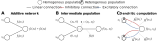
\includegraphics{media/chapter_multi_compartment_lif/nef_multivariate_functions.pdf}%
	{\phantomsubcaption\label{fig:nef_multivariate_functions_a}}%
	{\phantomsubcaption\label{fig:nef_multivariate_functions_b}}%
	{\phantomsubcaption\label{fig:nef_multivariate_functions_c}}%
	\caption[Using dendritic computation to compute multivariate functions in the NEF]{Using dendritic computation to compute multivariate functions in the NEF. \textbf{(A)} Standard NEF networks are additive: summation in activity space corresponds to addition in representation space.
	\textbf{(B)} Computing nonlinear multivariate functions $\phi$ generally requires all variables to be represented in an intermediate population.
	\textbf{(C)} The dendritic computation scheme discussed in here.
	Two pre-populations project onto a post-population with separate excitatory and inhibitory input channels.
	%The nonlinear interaction between these channels is exploited to compute $\phi$.
	}
	\label{fig:nef_multivariate_functions}
\end{figure}

The idea of dendritic computation as pursued here is best explained by exploring how mul\-ti\-va\-ri\-ate functions such as $\phi(x_1, \ldots, x_\ell)$ can be computed in the NEF, and by reviewing some fundamental theoretical properties of neural networks.
Specifically, we analyse three different network architectures (cf.~\Cref{fig:nef_multivariate_functions}).
\enquote{Additive networks} represent the variables $x_1$, $\ldots$, $x_\ell$ in independent neuron populations and cannot approximate most multivariate functions.
In contrast, networks with an intermediate population representing all variables at the same time are universal function approximators.
Dendritic computation relies on non-linear interaction between independent neural input channels.
While not as powerful as networks with an intermediate population, dendritic computation can approximate larger classes of functions well compared to additive networks.

\subsection{Additive Multivariate Networks}
\label{sec:additive_net}

As stated above, our goal is to compute multivariate functions $\phi(x_1, \ldots, x_\ell)$ within the context of the NEF.
%For the sake of simplicity, we mostly discuss bivariate functions of the form $\phi(x_1, x_2)$, but the same considerations apply to more than two input variables as well.
For the sake of simplicity, assume that two pre-populations representing the variables $x_1$, $x_2$ are connected to a common post-population.
To compute $\phi(x_1, x_2)$, we must find connection weights $\vec w_{1, i}$, $\vec w_{2, i}$ such that the following holds for every post-neuron $i$
\begin{align}
	a_i(\phi(x_1, x_2))
		= G_i \bigl[
			\langle \vec e_i, \phi(x_1, x_2) \rangle
		\bigr]
		\supposedEq G_i\bigl[
			\langle \vec w_{1, i}, \vec a^\mathrm{pre}_1(x_1) \rangle + \langle \vec w_{2, i}, \vec a^\mathrm{pre}_2(x_2)
		\rangle\bigr] \,.
	\label{eqn:nef_multivariate_addition}
\end{align}
Here, $a_i$ is the desired post-neuron activity according to the normative tuning-curve constraint (eq.~2.??).
% TODO: Add correct reference
As discussed in the context of the NEF transformation principle in Section~2.3.5, we assume that the current-translation function $J_i$ is part of the individual neuron response curve $G_i$, and that the currents induced by the pre-populations are summed.
% TODO: Add correct reference

Now, consider multivariate functions that can be decomposed into a sum of two univariate functions, i.e., $\phi(x_1, x_2) = f_1(x_1) + f_2(x_2)$ (\Cref{fig:nef_multivariate_functions_a}).
We can easily find weights $\vec w_{1, i}$, $\vec w_{2, i}$ that approximate such a function using the encoder-decoder split of the NEF.
Computing function decoders $\mat D^{f_1}$, $\mat D^{f_2}$ and using the identity $(\vec w_i)^T = \vec e_i \mat D$, we have
\begin{align*}
	G_i\bigl[
	  \langle
	  	\vec e_i \mat D^{f_1},
	  	\vec a^\mathrm{pre}_1(x_1)
	  \rangle
	+ \langle
	  	\vec e_i \mat D^{f_2},
		\vec a^\mathrm{pre}_2(x_2)
	\rangle\bigr] = 
	G_i\bigl[\langle \vec e_i, \mat D^{f_1} \vec a_1^\mathrm{pre}(x_1) + \mat D^{f_2} \vec a_2^\mathrm{pre}(x_2) \rangle\bigr]
	\approx a_i\bigl(f_1(x_1) + f_2(x_2)\bigr) \,.
\end{align*}
This equation can be interpreted as saying that addition in activity space (i.e., summing weighted pre-activities, eq.~\ref{eqn:nef_multivariate_addition}) is equal to addition in represented space.
In other words, standard NEF networks are \emph{additive}.
%\footnote{We already used the additivity of NEF networks in~Section~2.3.5, when we discussed the dynamics principle.}
Summing functions incurs no additional decoding error.

\begin{figure}
	\centering
	\includegraphics{media/chapter_multi_compartment_lif/perceptron.pdf}%
	{\phantomsubcaption\label{fig:perceptron_a}}%
	{\phantomsubcaption\label{fig:perceptron_b}}%
	\caption[Additive networks are a generalisation of the perceptron]{Additive networks are a generalisation of the perceptron. \textbf{(A)} An additive network is a sum of arbitrary univariate functions. \textbf{(B)} A perceptron is an additive network with functions of the form $f_i(x_i) = w_i x_i + \beta \ell^{-1}$. The weights $w_i$ are learned such that the output approximates a desired function.}
\end{figure}

\subsubsection{Additive networks cannot compute most multivariate functions}
The only way to compute general multivariate functions $\phi(x_1, x_2)$ in additive networks is to \emph{approximate} $\phi$ as an additive univariate decomposition.
As expressed by the following theorem (see Appendix~B.3.1 for a proof), it is \emph{impossible} to compute many continuous multi-variate $\phi$ using such additive networks.%
\footnote{We limit Theorem~\ref{thm:xor_general} to continuous functions for the sake of simplicity.
However, we conjecture that the same results hold for larger classes of functions, for example square Lebesgue integrable functions.}
This is true even if we can decode arbitrary univariate functions $f_1$, $\ldots$, $f_\ell$ over the pre-variables (this is equivalent to having an infinite number of pre-neurons, see below), and we were able to freely choose a fixed nonlinearity $\sigma$ (cf.~\Cref{fig:perceptron_a}).

\begin{theorem}
\label{thm:xor_general}
Let $\ell > 1$, $\Xrepr \subset \mathbb{R}^\ell$ and $\mathbb{Y} \subset \mathbb{R}$ be compact sets, and $\sigma$, $\phi$, $f_i$ be continuous.
For any fixed $\sigma : \mathbb{R} \longrightarrow \mathbb{Y}$, there always exist $\phi : \Xrepr \longrightarrow \mathbb{Y}$ such that there are no $f_1$, $\ldots$, $f_\ell : \mathbb{R}  \longrightarrow \mathbb{R}$ with the property
$\phi(x_1, \ldots, x_\ell) = \sigma(\xi) = \sigma\bigl( f_1(x_1) + \ldots + f_\ell(x_\ell) \bigr)$ for all $(x_1, \ldots, x_\ell) \in \Xrepr$.
\end{theorem}

\begin{figure}
	\centering
	\includegraphics{media/chapter_multi_compartment_lif/xor_visualisation.pdf}%
	{\phantomsubcaption\label{fig:xor_visualisation_a}}%
	{\phantomsubcaption\label{fig:xor_visualisation_b}}%
	{\phantomsubcaption\label{fig:xor_visualisation_c}}%
	{\phantomsubcaption\label{fig:xor_visualisation_d}}%
	{\phantomsubcaption\label{fig:xor_visualisation_e}}%
	\caption[Visualisation of the XOR decision problem for different classifiers]{Visualisation of the XOR decision problem for different classifiers. The goal is to find classifier parameters such that the four samples are classified as depicted.
	The background corresponds to the sign of the monotonic function $\sigma(\xi)$.
	\textbf{(A)} The linear decision boundary formed by the Perceptron cannot solve the XOR problem.
	\textbf{(B)} This holds for any function of the form $\sigma(f_1(x_1) + f_2(x_2))$, here $f_1(x_1) = \cos(2\pi x_1)$ and $f_2(x_2) = \sin(2\pi x_2)$.
	\textbf{(C)} A multi-layer Perceptron (MLP) of the form $\sum_i w_i \sigma(e_i^1 x_1 + e_i^2 x_2 + \beta_i )$ can solve the problem, although the decision boundary is quite erratic.
	\textbf{(D)} An alternative solution using the nonlinearity $\sigma'(\xi) = \sigma(\xi^2 - 1)$.
	\textbf{(E)} Multiplication of two real-valued variables $x_1$, $x_2$ can be seen as a continuous form of the XOR problem.
	Additive networks cannot compute this function.
	}
	\label{fig:xor_visualisation}
\end{figure}

\subsubsection{The Perceptron and XOR}
Consider monotonic $\sigma$ and affine $f_i$ of the form $w_i x_i + \beta \ell^{-1}$.
We obtain the \emph{perceptron}, an early single-layer neural network (cf.~\Cref{fig:perceptron_b}; \cite{rosenblatt1958perceptron}).
\Citet[Chapter~2; originally published in 1969]{minsky1987perceptrons} point out that such networks cannot compute the boolean XOR function (\Cref{fig:xor_visualisation_a}).%
\footnote{\Citet{minsky1987perceptrons} note that the perceptron was proved by Rosenblatt to \enquote{learn to do anything it was possible to program it to do}; this ambiguous statement endowed researchers with a surplus of optimism---especially since perceptrons could sometimes learn to solve difficult problems.
Among other factors, realising that these networks could not be \emph{programmed} to solve a simple problem such as XOR led to what some call \enquote{the first AI winter} \citep[e.g.,][]{muthukrishnan2020brief}.}
%In the continuous domain, the same is true for multiplication over $\mathbb{X} = [-1, 1]^2$, that is $\phi(x_1, x_2) = x_1 x_2$ (\Cref{fig:xor_visualisation_a}).
Even the general additive networks from our theorem cannot solve a \emph{weaker} version of the XOR problem, formalised below.

\begin{definition}
\label{def:weak_xor}
A function $\phi(x, y)$ solves the \emph{weak XOR problem} if there exist $a_0, b_0, a_1, b_1$ with
\begin{align*}
	\big( \phi(a_0, b_0) < \phi(a_0, b_1) \big) \wedge
	\big( \phi(a_1, b_1) < \phi(a_0, b_1) \big) \wedge
	\big( \phi(a_0, b_0) < \phi(a_1, b_0) \big) \wedge
	\big( \phi(a_1, b_1) < \phi(a_1, b_0) \big) \,.
\end{align*}
\end{definition}
That is, we merely require $\phi(a_0, b_0)$ and $\phi(a_1, b_1)$ to be larger than $\phi(a_0, b_1)$ and $\phi(b_1, b_0)$.

\begin{restatable}{theorem}{ThmWeakXor}
\label{thm:weak_xor}
Let $\sigma$ be monotonic. Then, an additive network of the form $\phi(x_1, x_2) = \sigma(f_1(x_1) + f_2(x_2))$ cannot solve the weak XOR problem.
\end{restatable}
This may be surprising, given that, as depicted in \Cref{fig:xor_visualisation_b}, we can generate highly nonlinear classification boundaries.
We provide a proof in Appendix~B.3.2.

To solve the XOR problem, we can either, as discussed next, use multi-layer networks (cf.~\Cref{fig:xor_visualisation_c}), or, alternatively make $\sigma$ non-monotonic.
As depicted in \Cref{fig:xor_visualisation_d}, setting $\sigma(\xi) = \xi^2 - 1$ allows us to solve the XOR problem.
This illustrates our goal with dendritic computation: exploit \enquote{more powerful} $\sigma$ to approximate a larger class of functions.

Still, the functions that we can compute using additive networks are limited, even if we can freely choose $\sigma$.
For example, we can compute $x_1 x_2$ for $(x_1, x_2) \in [\epsilon, 1]^2$ and $0 < \epsilon < 1$ by setting $f_1$ and $f_2$ to the logarithm and $\sigma$ to the exponential.
However, it is impossible to find functions that compute multiplication over all four quadrants---which can be seen as a continuous version of the XOR problem (\Cref{fig:xor_visualisation_e}).
More precisely, allowing $x_1$, $x_2$ to be zero makes it impossible to compute multiplication in these networks (proof in Appendix~B.3.3).
\begin{restatable}{theorem}{ThmMultiplication}
\label{thm:multiplication}
There are no continuous, real-valued functions $f_1$, $f_2$, $\sigma$ such that $\sigma(f_1(x_1) + f_2(x_2)) = x_1 x_2$ for all $(x_1, x_2) \in [0, 1]^2$.
\end{restatable}


%Choosing this $\sigma$ implicitly introduces a non-linear interaction between the variables $x_1$, $x_2$, for example
%\begin{align*}
%	\sigma\left( (w_1 x_1 + w_2 x_2 + \beta)^2 - 1\right) = 
%	\sigma\left( w_1^2 x_1^2 + w_2^2 x_2^2 + 2 w_1 w_2 x_1 x_2 + 2 w_1 \beta x_1 + 2 w_2 \beta x_2 + \beta^2  - 1\right) \,.
%\end{align*}
%The product-term $w_1 w_2 x_1 x_2$ can be exploited to %compute multiplication-like functions.
%Still, as stated in Theorem~1, there inevitably is a large set of functions that we cannot compute.
% TODO Add reference

\subsection{Multi-Layer Networks}

\begin{figure}
	\includegraphics{media/chapter_multi_compartment_lif/mlp.pdf}
	\caption[Sketch of a two-layer neural network]{Sketch of a two-layer neural network with rectified linear units (ReLUs). If the encoding vectors $\vec e_i$ and the biases $\beta_i$ are sampled appropriately, this network is a universal function approximator.}
	\label{fig:mlp}
\end{figure}

As already mentioned in Section~2.3.5, an individual NEF population can be interpreted as a two-layer neural network (cf.~\Cref{fig:mlp}).
% TODO: Add reference
As long as the encoding vectors are sampled from $\ell$-dimensional hypersphere and $x$-intercepts are uniformly distributed, such a neuron population is a universal function approximator.
The following theorem states this more formally for neurons with a rectified linear unit (ReLU) nonlinearity, i.e., $\sigma(\xi) = \max\{0, \xi\}$.

\begin{theorem}
\label{thm:two_layer_universal}
Let $\ell \geq 1$, and $\phi : \mathbb{B}^\ell \longrightarrow \mathbb{R}$ be a continuous function mapping from the $\ell$-dimensional unit ball onto $\mathbb{R}$.
Furthermore, let $\sigma(\xi) = \max\{0, \xi\}$, $\vec e_i$ be sampled uniformly from the unit-sphere $\mathbb{S}^\ell$, and $\beta_i$ be sampled uniformly from $[-1, 1]$.
There exist $d_i \in \mathbb{R}$ such that
\begin{align}
	\phi(\vec x) = \lim_{\Npop \to \infty} \sum_{i = 1}^{\Npop} d_i \sigma\bigl( \langle \vec e_i, \vec x \rangle + \beta_i \bigr) \quad \text{for all} \quad \vec x \in \mathbb{B}^\ell \,.
	\label{eqn:two_layer_network}
\end{align}
\end{theorem}

This follows from \citet{hornik1989multilayer}.
We provide a sketch of a proof in Appendix~B.3.3.
This theorem can be easily extended to hold for arbitrary compact domains $\Xrepr$, codomain dimensionalities, and other neural nonlinearities $\sigma$.

%It may not be obvious why \cref{eqn:two_layer_network} describes a \enquote{two-layer} neural network.
%In essence, the encoding weights $\vec e_i$ map $\vec x$ onto the input of one of the $N$ neurons with nonlinearity $\sigma$.
%This step forms the \enquote{first} or \enquote{hidden layer}.
%The decoding weights $d_i$ then map the neural activities $\sigma(\xi_i)$ onto the output, which forms the \enquote{second layer} (cf.~Figure~2.20).
%% TODO: Add actual reference

\subsubsection{The role of uniformly sampled encoders}
Theorem~\ref{thm:two_layer_universal} requires that the encoding vectors $\vec e_i$ are uniformly sampled from the hypersphere $\mathbb{S}^\ell$.%
\footnote{As follows from the proof of Theorem~\ref{thm:two_layer_universal} in Appendix~B.3.3, there technically are weaker requirements for this.
One example is given in \citet{gosmann2015precise}; given a specific function $\phi$ (such as multiplication), there are certain distributions of encoding vectors that minimise the decoding error.
In fact, global optimisation methods such as stochastic gradient descent can be seen as systematically selecting such \enquote{optimal} encoders.}
To get an intuition as for why this is important, consider the case where the $\vec e_i$ are axis-aligned, i.e., $\|\vec e_i\|_0 = 1$ (cf.~Appendix~A.1).
% TODO: Add reference for zero-norm in Appendix~A.1
In this case, we can split \cref{eqn:two_layer_network} into $\ell$ sub-networks, each decoding a function over a single variable $x_\ell$
\begin{align*}
		\sum_{i = 1}^N d_i \sigma\bigl( \langle \vec e_i, \vec x \rangle - \beta_i \bigr)
	= 	\sum_{j = 1}^\ell \sum_{i = 1}^{N_j} d_{j i} \sigma\bigl( e_{j i} x_j - \beta_{j i} \bigr) \,, \text{where } e_{j i} \in \{ -1, 1\} \,.
\end{align*}
This is equivalent to the additive networks we discussed before.
We can only decode sums of univariate functions over the individual $x_j$ from the pre-population.

\subsubsection{Intermediate populations}
%We now know that we can indeed approximate multivariate functions in the NEF with an arbitrarily small error.
%The pre-condition for this is that all variables over which we would like to compute a $\phi$ represented in the same neuron population with non-axis aligned encoding vectors $\vec e_i$.
As discussed by \citep[Chapter~6]{eliasmith2003neural}, we need to introduce intermediate populations if, as an example, variables $x_1$, $x_2$ are represented in independent pre-populations, and we would like to compute a multivariate function $\phi(x_1, x_2)$.
This intermediate population represents a vectorial quantity $\vec z = (x_1, x_2)$ (cf.~\Cref{fig:nef_multivariate_functions_b}).
This can be accomplished by computing the univariate functions $f_1(x_1) = (x_1, 0)$ and $f_2(x_2) = (0, x_2)$ in the connections to the intermediate population.
According to Theorem~\ref{thm:two_layer_universal} we can then decode any multivariate function from the intermediate population.

\subsubsection{Potential issues with intermediate populations}
In theory, the number of neurons required to cover a $d$-dimensional space is exponential in $d$.
Representing a $d$-dimensional quantity in an intermediate population thus requires many neurons to achieve a certain decoding error.
In practice, it is quite difficult to judge the number of neurons required to decode a certain function $f$ a-priori; the decoding error heavily depends on $f$ and the encoding vectors $\vec e_i$.

Another problem arises when modelling neurobiological systems.
There may be no indication that an intermediate population exists in a particular biological circuit, but the function can be modelled well as a multivariate function.
An example of this would be the aforementioned attention system, where a group of control neurons modulates another population without an intermediary \citep{bobier2014unifying}.

Finally, there is the issue of noise.
In spiking neural networks, every intermediate neuron population introduces additional noise due to static distortion and spike noise \citep[Section~2.2.2]{eliasmith2003neural}.
We see the effects of this later.

\subsection{Dendritic Computation}
\label{sec:dendritic_computation_theory_dendritic}

Dendritic computation is one way to partially alleviate the limitations arising from intermediate populations.
The basic idea is that each neuron possesses $k$ \emph{input channels}.
Input fed through these channels interacts nonlinearly, modelling information processing within the dendrites.

\begin{figure}
	\includegraphics{media/chapter_multi_compartment_lif/dendritic_computation.pdf}%
	{\phantomsubcaption\label{fig:dendritic_computation_net}}%
	{\phantomsubcaption\label{fig:dendritic_computation_fun}}%
	\caption[Overview of our notion of dendritic computation.]{Overview of our notion of dendritic computation. \textbf{(A)} Neuron with an excitatory and inhibitory input channel. In a network context, these functions are decoded from pre-populations representing these variables. Connectivity can be constrained such that excitatory and inhibitory pre-neurons only connect to the corresponding channel. \textbf{(B)} Conceptually, each channel receives a sum of univariate functions computed over the pre-variables $x_1$, $\ldots$, $x_\ell$.}
\end{figure}

Mathematically, the response curve describing the average neural activity is now a multivariate function $\mathscr{G}[\xi_1, \ldots, \xi_k]$, where the $\xi_i$ are linear combinations of the pre-activities (\Cref{fig:dendritic_computation_net}).
To compute $\phi(x_1, \ldots, x_\ell)$, the following must hold for each post-neuron $i$
\begin{align}
	\begin{aligned}
	a_i\bigl(\phi(x_1, \ldots, x_\ell)\bigr) &\supposedEq
	\mathscr{G} \bigl[
		\langle \vec w_{1, i}^1, \vec a^\mathrm{pre}_1(x_1) \rangle + \ldots +
		\langle \vec w_{\ell, i}^1, \vec a^\mathrm{pre}_\ell(x_\ell) \rangle, \ldots,\\
%	&~\quad\quad\vdots, \\
	&~\hspace{1.66em}
		\langle \vec w_{1, i}^k, \vec a^\mathrm{pre}_1(x_1) \rangle + \ldots +
		\langle \vec w_{\ell, i}^k, \vec a^\mathrm{pre}_\ell(x_\ell) \rangle
	\bigr]
	\end{aligned}
	\label{eqn:dendritic}
\end{align}
where $a_i(\phi(x_1, \ldots, x_\ell))$ expresses the normative tuning constraint defined in Section~2.3.2.
% TODO: Add correct reference

Note that we deliberately left the concept of an \enquote{input channel} a little vague.
An input channel could either refer to a different location in the dendritic tree, different synapse types (e.g., excitatory or inhibitory synapses), or even the effects of signalling molecules such as hormones.
We discuss examples of model neurons with multiple input channels in \Cref{sec:nlif}.

\subsubsection{Mathematical analysis}
More formally, using $\sigma(\xi_1, \ldots, \xi_\ell)$ as an abstract nonlinearity and assuming that we can compute any univariate function $g_i^j$ over $\xi_1, \ldots, \xi_\ell$, we have (\Cref{fig:dendritic_computation_fun})
\begin{align}
	\sigma \bigl(
		g_{1}^1(x_1) + \ldots + g_{\ell}^1(x_\ell), \ldots, g_{1}^k(x_1) + \ldots + g_{\ell}^k(x_\ell)
	\bigr) = \phi(x_1, \ldots, x_\ell) \,.
	\label{eqn:dendritic_computation_theory}
\end{align}
Such networks are more powerful than additive networks.
For example, let $\sigma(\xi_1, \xi_2) = \xi_1 \xi_2$.
Now, if we set the functions feeding into the second channel to one, i.e., $g_{1, i}^2(x_1) = \ldots = g_{\ell, 1}^2(x_\ell) = 1$, we obtain an additive network.
Of course, using the same $\sigma$, we can, in contrast to additive networks, compute products of the pre-variables over arbitrary domains.

Still, independent of $\sigma$, and similarly to additive networks, dendritic computation networks are not universal function approximators (see Appendix~B.3.5~for the theorem and proof).

%\begin{theorem}
%\label{thm:dendritic_compuation_incomplete}
%Let $\ell > 1$, $\Xrepr \subset \mathbb{R}^\ell$ and $\mathbb{Y} \subset \mathbb{R}$ be compact sets, and $\sigma$, $\phi$, $g^j_i$ be continuous.
%For any fixed $\sigma : \mathbb{R}^k \longrightarrow \mathbb{Y}$, there always exist $\phi : \Xrepr \longrightarrow \mathbb{Y}$ such that there are no $g^1_1$, $\ldots$, $g^k_\ell : \mathbb{R}  \longrightarrow \mathbb{R}$ with the property
%$\phi(x_1, \ldots, x_\ell) = \sigma(\xi_1, \ldots, \xi_k) = \sigma\bigl( g^1_1(x_1) + \ldots + g^1_\ell(x_\ell), \ldots,  g^k_1(x_1) + \ldots + g^k_\ell(x_\ell)\bigr)$ for all $(x_1, \ldots, x_\ell) \in \Xrepr$.
%\end{theorem}

%\subsubsection{Interaction between excitation and inhibition}
%\Cref{fig:nef_multivariate_functions_c} shows an example of a neural network exploiting nonlinear interactions between excitatory and inhibitory synapses.
%Assume that each neuron in the post population possesses an independent excitatory and inhibitory channel, and that the two pre-population represent $x_1$, $x_2$, respectively, and project onto both channels.
%The activity of a single post-neuron $i$ is hence given as
%\begin{align*}
%	\mathscr{G}_i\bigl[
%		\langle
%			\vec w^1_\mathrm{E},
%			\vec a_\mathrm{pre}^1(\vec x_1)
%		\rangle + \langle
%			\vec w^2_\mathrm{E},
%			\vec a_\mathrm{pre}^2(\vec x_2)
%		\rangle,
%		\langle
%			\vec w^1_\mathrm{I},
%			\vec a_\mathrm{pre}^1(\vec x_1)
%		\rangle + \langle
%			\vec w^2_\mathrm{I},
%			\vec a_\mathrm{pre}^2(\vec x_2)
%		\rangle
%	\bigr] \,,
%\end{align*}
%where $\vec w_\mathrm{I}$ and $\vec w_\mathrm{E}$ are the excitatory and inhibitory synaptic weights, and $\vec a_\mathrm{pre}$ are the activities of the pre-populations.
%Assuming that we can decode arbitrary univariate functions over $x_1$, $x_2$ from the pre-populations, our goal is to find functions $g_\mathrm{E}^1(x_1)$, $g_\mathrm{E}^2(x_2)$, $g_\mathrm{I}^1(x_1)$, $g_\mathrm{I}^2(x_2)$, such that the total activity of our neuron has some desired value, i.e.,
%\begin{align*}
%	a_i^\mathrm{post}(\phi(x_1, x_2)) \supposedEq \mathscr{G}_i\bigl[
%		g_\mathrm{E}^1(x_1) + g_\mathrm{E}^2(x_2),
%		g_\mathrm{I}^1(x_1) + g_\mathrm{I}^2(x_2)
%	\bigr] \,.
%\end{align*}


\subsection{Numerical Exploration}
\label{sec:dendritic_computation_theory_numerical}

The above considerations are quite theoretical and provide only limited insight into the practical impact of choosing one network type over the other.
In this section, we discuss a simple numerical experiment that highlights the function approximation errors obtained with different network types for functions $\phi$ of varying \enquote{complexity}.
We use experiments similar to the following throughout this chapter to characterise different network- and neuron-types.

\begin{figure}
	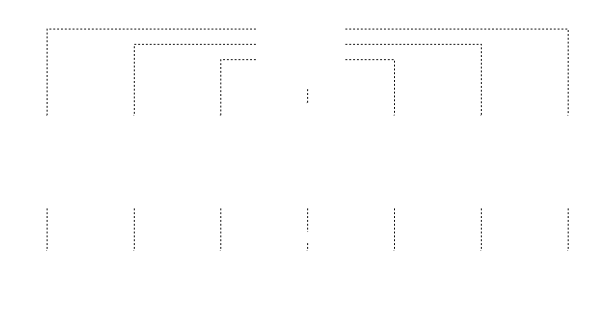
\includegraphics{media/chapter_multi_compartment_lif/2d_functions_overview_overlay.pdf}%
	\kern-157.24mm\includegraphics{media/chapter_multi_compartment_lif/2d_functions_overview.pdf}
	\caption[Overview of our procedure for generating random 2D functions]{Overview of our procedure for generating random 2D functions. \textbf{(A)} We sample a 2D array from a normal distribution (size of the array depends on the filter width; negative values in red, positive in blue). \textbf{(B)} The noise is filtered by convolving with a Gaussian kernel with standard-deviation $\sigma$ (for large filter widths, i.e., small $\sigma^{-1}$, only a small portion of the filter is depicted). \textbf{(C)} The resulting functions are transformed to have mean zero (i.e., no DC component) and a standard deviation of one.}
	\label{fig:2d_functions_overview}
\end{figure}

To analyse different network architectures, w
e randomly generate two-dimensional functions $\phi(x_1, x_2)$ from band-limited white noise with standard deviation one and mean zero.
The band-limit is enforced by filtering with a Gaussian filter kernel with standard deviation $\sigma$.
This is depicted in \Cref{fig:2d_functions_overview}.
Large $\sigma$ result in functions with no high frequencies; such functions are approximately linear.
In contrast, small $\sigma$ result in quite intricate random structures.
Correspondingly, $\sigma^{-1}$ can be seen as a proxy for the \enquote{complexity} of a function.
Small $\sigma^{-1}$ result in low-complexity functions, large $\sigma^{-1}$ in high-complexity functions.


\clearpage

\section{Extending the Neural Engineering Framework}

Up to this point, we have formally defined dendritic computation and discussed its theoretical benefits.
The goal of this section is to open avenues toward systematically integrating multi-compartment neuron models with dendritic trees into NEF networks using the formalisms discussed above.

Na\"ively, incorporating neurons with multiple nonlinear input channels into the NEF is merely a matter of solving for $\vec w$ such that \Cref{eqn:dendritic} holds.
Phrasing this as an optimization problem, we must minimise the difference between the desired average activity according to the normative tuning-curve constraint $a_i(\vec x)$ and the average activity according to our multi-variate response curve $\mathscr{G}$.
Using a least-squares loss (and omitting the regularisation term), we have
\begin{align}
	\begin{aligned}
	E &=
	\frac{1}{\vol(\Xrepr)} \int_{\Xrepr} \Bigl( a_i\bigl(\phi(x_1, \ldots, x_\ell)\bigr) -
	\mathscr{G} \bigl[
		\langle \vec w_{1, i}^1, \vec a^\mathrm{pre}_1(x_1) \rangle + \ldots +
		\langle \vec w_{\ell, i}^1, \vec a^\mathrm{pre}_\ell(x_\ell) \rangle, \ldots,\\
	&~\hspace{13.825em}
		\langle \vec w_{1, i}^k, \vec a^\mathrm{pre}_1(x_1) \rangle + \ldots +
		\langle \vec w_{\ell, i}^k, \vec a^\mathrm{pre}_\ell(x_\ell) \rangle
	\bigr] \Bigr)^2 \,dx_1 \ldots dx_\ell \,.
	\end{aligned}
	\label{eqn:dendritic_computation_optimisation}
\end{align}
On way to minimise this loss-function would be to use stochastic gradient descent.
In fact, this can be a viable strategy---and may be the only option for many detailed neuron models.

Still, we would like to suggest a more systematic approach that, in some cases, reduces the task of finding weights to a convex quadratic program.
This is more in line with the \enquote{standard} NEF, where connection weights are computed by solving a convex least-squares problem.

To arrive at a point where we can integrate complex neuron models more seamlessly, we first need to address two of the limitations of the NEF discussed in Section~2.3.5.
Specifically, we discuss how to eliminate the bias currents and to account for Dale's principle.
Furthermore, we present a modified version of \Cref{eqn:dendritic_computation_optimisation} that splits the multivarite response-curve $\mathscr{G}$ into a multivariate input-dependent nonlinearity $H$ and a univariate response-curve $G$.
We avoid decoding subthreshold currents using a technique we call \enquote{subthreshold relaxation}.

\subsection{Decoding the Current-Translation Function}
\label{sec:nef_decode_current}

So far we assumed that the current translation function $J_i(\xi)$ is an intrinsic part of the neuron model.
Our typical choice of $J_i(\xi) = \alpha_i \xi + \beta_i$ introduces a bias current $\beta_i$ into each neuron.
As we elaborated in Section~2.3.5, this is slightly implausible from a biological perspective.

\Citet{tripp2007neural} demonstrate that it is possible to robustly solve for synaptic weights that approximate arbitrary post-synaptic current functions.
We use this insight to directly approximate the target current $J_i(\langle \vec e_i, \vec x \rangle)$ and thus implicitly solve for the bias.
Again, assuming that the post-synaptic current is linear in the pre-population activities, we must find a weight vector $\vec w_i$ such that the following regularised loss is minimised
\begin{align}
E = \frac{1}{\vol(\Xrepr)} \int_{\Xrepr} \left( J_i\bigl(\langle \vec e_i, \phi(\vec x)\rangle\bigr) - \langle \vec w_i, \vec a^\mathrm{pre}(\vec x) \rangle \right)^2 \, d\vec x + \lambda \| \vec w_i \|_\mathrm{2}^2\,.
\label{eqn:decode_current}
\end{align}
As before, this equation can be discretised and brought into canonical least squares form and solved using the regularised Moore-Penrose pseudo inverse (cf.~eqn.~2.22 and 2.23):
\begin{align*}
	\mat W &= \mat A^+ \mat J \,, & \text{where} \quad \mat A^+ &= (\mat A^T \mat A + \lambda N \mat I)^{-1} \mat A^T \,.
\end{align*}
Here, $N$ is the number of samples, $\mat W \in \mathbb{R}^{m \times \Npop}$ is the connection weight matrix, $\mat J \in \mathbb{R}^{N \times m}$ is a matrix of target currents, and $\mat A \in \mathbb{R}^{N \times n}$ is the matrix of pre-activities.

\begin{figure}
	\includegraphics{media/chapter_multi_compartment_lif/current_translation_decoding.pdf}%
	{\phantomsubcaption\label{fig:current_translation_decoding_a}}%
	{\phantomsubcaption\label{fig:current_translation_decoding_b}}%
	{\phantomsubcaption\label{fig:current_translation_decoding_c}}%
	{\phantomsubcaption\label{fig:current_translation_decoding_d}}%
	\caption[Decoding for currents instead of represented values]{Decoding for currents instead of represented values. \textbf{(A)} Tuning curves of a pre-populations with $100$ LIF neurons (only $50$ tuning curves are shown). \textbf{(B)} Decoding affine current translation functions $J_i$ (black dotted lines are the target). The function $\phi$ being computed in re\-pre\-sen\-tat\-ion space is the identity function. Dashed line corresponds to the threshold current $J_\mathrm{th} = \SI{1}{\nano\ampere}$.
	\textbf{(C)} Same as \emph{(B)} but for Gaussian current-translation functions $J_i$. Such functions can be used to produce localised tuning curves.
	\textbf{(D)} First six singular values of the two weight matrices $\mat W$ from \emph{(B, C)}.
	Singular values are normalised by dividing by their sum, resulting in the relative contribution of each singular value to the decoding.
	For affine $J_i$, $\mat W$ is of rank $d + 1$ (here $d = 1$);
	Gaussian $J_i$ result in full-rank $\mat W$.
	}
\end{figure}

Importantly, we no longer solve for weights directly in the domain of represented values $\vec x$; this is in contrast to solving for decoders $\mat D$ according to eqn.~(2.??).
Similarly, we do not solve for target activities $a_i$, as was suggested by our na\"ive loss function in \cref{eqn:dendritic_computation_optimisation}.
Side-stepping the neural nonlinearity $G$ enables a simple least-squares solution.
Furthermore, this optimisation scheme supports arbitrary current-translation functions $J_i$, providing modellers with a greater flexibility over the tuning curve constraint (cf.~\Cref{fig:current_translation_decoding_a,fig:current_translation_decoding_b,fig:current_translation_decoding_c}).

\subsubsection{Low-rank factorisation of $\mat W$}
Solving the optimisation problem in \cref{eqn:decode_current} directly results in weight matrix $\mat W$ instead the low-rank factorisation $\mat W = \mat E \mat D^\phi$.
As we discussed in Section~???, this factorisation was useful, as it enables $\mat W \vec a$ to be computed in $\mathcal{O}(n)$ instead of $\mathcal{O}(n^2)$.

Fortunately, at least in the case of the affine current-translation function $\alpha_i \langle \vec e_i, \phi(\vec x) \rangle + \beta_i$, we still obtain a factorisable matrix (cf.~\Cref{fig:current_translation_decoding_d}).
The resulting $\mat W$ is merely of rank $d + 1$, where $d$ is the dimensionality of the post-population.
Specifically, the weight matrix can be expressed as a sum of the low-rank factorisation $\mat E \mat D^\phi$ and the outer product of the biases $\vec \beta \in \mathbb{R}^{m \times 1}$ with a decoding vector $\mat D^1 \in \mathbb{R}^{1 \times n}$.
This \enquote{bias-decoder} decodes the constant \enquote{one} from the pre-population.
In other words, it simply holds $\mat W = \mat E \mat D^\phi + \vec \beta \mat D^1$ (cf.~\cite[Chapter~4]{stockel2017point,duggins2017incorporating}).

\begin{figure}
	\includegraphics{media/chapter_multi_compartment_lif/bias_decoding_impact.pdf}%
	{\phantomsubcaption\label{fig:bias_decoding_impact_a}}%
	{\phantomsubcaption\label{fig:bias_decoding_impact_b}}%
	{\phantomsubcaption\label{fig:bias_decoding_impact_c}}%
	{\phantomsubcaption\label{fig:bias_decoding_impact_d}}%
	\caption[Bias decoding and post-population tuning curve accuracy]{Bias decoding and post-population tuning curve accuracy. \textbf{(A)} Pre-population tuning-curves for $n = 50$ LIF neurons.
	\textbf{(B)}~Error for decoding the identity function compared to decoding a constant (regularisation factor $\sigma = 10$). The error for decoding a constant is minimally larger than that for decoding the identity function.
	\textbf{(C)}~The first four principal components of the tuning curves (for $n = 1000$).
	The principal components resemble the Legendre polynomials, an orthogonal function basis (dotted lines).
	\textbf{(D)} RMSE between the desired post-population tuning and the actually achieved tuning. Decoding the bias approximately doubles the error compared to intrinsic bias currents.}
\end{figure}

\subsubsection{Impact of decoding bias currents on network function}
%It is difficult to make blanket statements about the impact of bias decoding on the network function.
Generally speaking, decoding biases increases the error between the actual and desired post-population tuning.
The magnitude of this error depends on the pre- and post-population. 
The former determine how well a constant offset can be decoded, the latter determine the magnitude of the required bias currents.

In the case of \enquote{standard} NEF tuning with uniform $x$-intercepts and random encoders (cf.~\Cref{fig:bias_decoding_impact_a}), constant functions can, counter-intuitively, only be decoded with a slightly higher error than the identity function (error is about $15\%$ higher; cf.~\Cref{fig:bias_decoding_impact_b}).
This becomes apparent when considering the principal components of the pre-population tuning curves.
As for example discussed in \citet[Chapter~7]{eliasmith2003neural}, the principal component analysis (PCA) can be seen as \enquote{uncovering} the best orthogonal basis that linearly generates the tuning-curves.
%(see \cite[Chapter~12]{bishop2006pattern} for general information on the PCA).
In turn, the first principal components characterise the functions that can be decoded well from a population.
As illustrated in \Cref{fig:bias_decoding_impact_c}, the principal components $f_i$ of the \enquote{standard} NEF tuning curves resemble the Legendre polynomials (cf.~Section~4.? for a definition).
While the second principal component $f_2$ is linear, just like the corresponding Legendre polynomial, $f_1$ differs significantly from the constant first Legendre polynomial.
Decoding constants is hence \enquote{more difficult} than decoding the identity function.

In our example, and as depicted in \Cref{fig:bias_decoding_impact_d}, decoding $J_i$ doubles the RMSE between the desired and actual post-population tuning.
%This can be countered by doubling the number of pre-neurons.
However, as we will see in the next subsection, there are circumstances where the absence of an intrinsic bias is beneficial to network performance.

\subsubsection{Accounting for multiple pre-populations}
As we discussed in \Cref{sec:additive_net}, a welcome side effect of intrinsic current-translation is that standard NEF networks are additive.
Summing the activities $\vec a^\mathrm{pre}_1$, $\ldots$, $\vec a^\mathrm{pre}_\ell$ from multiple pre-populations is equivalent to summing the decoded $f_1(\vec x_1)$, $\ldots$, $f_\ell(\vec x_\ell)$.
This is no longer the case when
%solving for weights $\vec w_i$
minimising the current-based loss in \cref{eqn:decode_current}.

\begin{figure}
	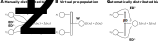
\includegraphics{media/chapter_multi_compartment_lif/nef_decode_bias.pdf}%
	{\phantomsubcaption\label{fig:nef_decode_bias_a}}%
	{\phantomsubcaption\label{fig:nef_decode_bias_b}}%
	{\phantomsubcaption\label{fig:nef_decode_bias_c}}%
	\caption[Accounting for multiple pre-populations when decoding the current-translation function.]{Accounting for multiple pre-populations when decoding the current-translation function. \textbf{(A)} Biases can be manually distributed between pre-populations by scaling the bias decoders $\mat D^1_1$ and $\mat D^1_2$ by $\alpha$ and $(1 - \alpha)$, respectively. \textbf{(B)} The general solution is to solve for weights $\mat W$ assuming stacked pre-population activities. The two pre-populations form a \enquote{virtual} pre-population. \textbf{(C)} A combination of the two approaches, where only the bias $\mat D^1$ is decoded from the pre-populations in this way.}
\end{figure}

In the case of the affine $J_i$, each of the $\ell$ connections decodes the bias current, effectively multiplying the bias by $\ell$.
Of course, we can only decode a fraction of the bias from each pre-population (\Cref{fig:nef_decode_bias_a}).
Alternatively, we can combine the pre-populations into a \enquote{virtual pre-population} and let the optimisation process take care of distributing the responsibility for providing the bias between all pre-neurons (\Cref{fig:nef_decode_bias_b}).

More precisely, we explicitly solve for weights that result in $f_1(\vec x_1) + \ldots + f_\ell(\vec x_\ell)$ to be represented in the post-population.
For two populations, and skipping regularisation, we have
\begin{align}
	E =
	\frac{1}{\vol(\Xrepr)^2} \! \iint_{\Xrepr}
	\left(
		J_i\bigl(\langle \vec e_i, f_1(\vec x_1) + f_2(\vec x_2) \rangle\bigr)
		- \langle \vec w_{1, i}, \vec a_1^\mathrm{pre}(\vec x_1) \rangle
		- \langle \vec w_{i, 2}, \vec a_2^\mathrm{pre}(\vec x_2) \rangle
	\right)^2 \, d\vec x_1 d\vec x_2 \,.
	\label{eqn:decode_current_additive}
\end{align}
We can bring this problem into a canonical form by the stacking the pre-activities and weights (see below for an example).
However, note that we now need to sample a much higher-dimensional space.
This is worrisome if we attempt to decode $f_i$ that must be finely sampled to obtain a good decoding.
Again, under the assumption that $J_i$ is affine, it is possible to expand the above integral and to solve for an---relatively easy to decode---population-spanning bias decoder $\mat D^1$ independent of the (untouched) function decoders $\mat D^{f_1}$ and $\mat D^{f_2}$ (\Cref{fig:nef_decode_bias_c}).

%\begin{align*}
%E^\beta &= \frac{1}{\vol(\Xrepr)^2} \! \int_{\Xrepr} \! \int_{\Xrepr} \left( \beta_i - \langle \vec w^\beta_{1, i}, \vec a_1^\mathrm{pre}(\vec x_1) \rangle - \langle \vec w^\beta_{i, 2}, \vec a_2^\mathrm{pre}(\vec x_2) \rangle \right)^2 \, d\vec x_1 \, d\vec x_2
%\end{align*}

\subsection{Nonnegative Weights and Dale's Principle}
\label{sec:nef_nonneg}

Biological neurons tend to follow Dale's principle---they act either excitatorily or inhibitorily (see~Section~2.2.1 for more detail).
As discussed in Section~2.3.6, we ignored this in our weight-solving procedures.
Least-squares assigns arbitrary algebraic signs to the individual weights, typically with an even split between positive and negative (cf.~Figure~2.33).
Such weights are not compatible with conductance-based synapses or, more generally, multi-compartment neurons.
Here, modellers connect pre-neurons to specific post-neuron channels.
The corresponding connection weights describe nonnegative quantities, such as the number of vesicles released from the pre-synapse, or the channel density in the post-synapse \citep{roth2009modeling}.
% TODO: Double-check citation

%While the concept of negative resistances and conductances exists, these are the result of active nonlinear processes not directly related to synaptic transmission \citep[e.g.,][]{bezanilla1972negative}.
%% TODO: Double-check source

\subsubsection{Solving for weights using non-negative least squares}
Solving for individual synaptic weights in current space suggests a simple procedure to account for nonnegativity.
Assume that each population is arbitrarily split into a group of excitatory and inhibitory neurons.
The somatic input current of post-neuron $i$ in response to pre-synaptic activity is $\langle \vec w_i^+, \vec a^+(\vec x) \rangle - \langle \vec w_i^-, \vec a^-(\vec x) \rangle$;
here, $\vec w_i^+$, $\vec w_i^-$ are nonnegative excitatory and inhibitory weight vectors and $\vec a^+(\vec x)$, $\vec a^-(\vec x)$ are the activities of the excitatory and inhibitory neurons in the pre-population.
Combining this current term with \cref{eqn:decode_current} yields the following optimisation problem for each post-neuron $i$
\begin{align}
	\begin{aligned}
	& \min_{{\vec w}_i^+, {\vec w}_i^-}
	\frac{1}{\vol(\Xrepr)} \int_{\Xrepr} \!
	\left(
		J_i\bigl(\langle \vec e_i, \phi(\vec x) \rangle\bigr)
		- \langle \vec w_{i}^+, \vec a^+(\vec x) \rangle
		+ \langle \vec w_{i}^-, \vec a^-(\vec x) \rangle
	\right)^2 \, d\vec x + \sigma^2 \|\vec w_{i}^+\|_2^2 + \sigma^2 \|\vec w_{i}^-\|_2^2 \\
	& \text{subject to } \vec w_i^+, \vec w_i^- \geq 0 \,.
	\end{aligned}
	\label{eqn:decode_nonneg}
\end{align}
To obtain a canonical least-squares form, let $N$ be the number of samples, $n^+$, $n^-$ be the number of excitatory and inhibitory pre-neurons%
\footnote{
It must not necessarily hold that $n = n^+ + n^-$; neurons can \emph{technically} be marked as both excitatory and inhibitory. Specifically, the special case $n = n^+ = n^-$ reduces the NNLS problem to standard least squares.
}%
, and $\mat A$ be the sampled, stacked, and signed pre-activities $(\mat A^+, -\mat A^-) \in \mathbb{R}^{N \times (n^+ + n^-)}$.
Additionally, let $\mat W$ be the stacked weight matrices $(\mat W^+, \mat W^-) \in \mathbb{R}^{m \times (n^+ + n^-)}$, and $\vec J \in \mathbb{R}^{N \times m}$ be a matrix of sampled target currents. We have
\begin{align}
	\bigl\| \bigl( \mat A^T \mat A + N \sigma^2 \mat I \bigr) \mat W - \mat A^T \mat J \bigr\|_2^2 \quad\quad \text{subject to } \mat W \geq 0 \,.
	\label{eqn:decode_nonneg_canon}
\end{align}
This is a standard nonnegative least-squares (NNLS) problem that can be solved in polynomial time \citep[Chapter~23]{lawson1995solving}.
An overview of efficient algorithms to solve this kind of problem is given in \citet{chen2009nonnegativity}.%
\footnote{Most linear algebra software packages bundle a solver for nonnegative least-squares; for example \texttt{scipy.optimize.nnls} in SciPy or \texttt{lsqnonneg} in Matlab. Alternatively, a gernal quadratic programming (QP) solver can be used; this is what we do in our library \texttt{libbioneuronqp} that we discuss at the end of this chapter.}
Of course, similarly to \cref{eqn:decode_current_additive}, the optimisation problem can be extended to take multiple pre-populations into account.

\begin{figure}[p]
	\centering
	
\includegraphics{media/chapter_multi_compartment_lif/nonnegative_experiments_setup.pdf}\\[0.75cm]	\includegraphics{media/chapter_multi_compartment_lif/nonnegative_experiments.pdf}\\[0.75cm]
	\includegraphics{media/chapter_multi_compartment_lif/nonnegative_experiments_tuning.pdf}%
	{\phantomsubcaption\label{fig:nonnegative_experiments_a}}%
	{\phantomsubcaption\label{fig:nonnegative_experiments_b}}%
	{\phantomsubcaption\label{fig:nonnegative_experiments_c}}%
	{\phantomsubcaption\label{fig:nonnegative_experiments_d}}%
	{\phantomsubcaption\label{fig:nonnegative_experiments_e}}%
	\caption[Impact of the ratio between excitatory to inhibitory neurons on network function]{Impact of the ratio between excitatory to inhibitory neurons on network function.
	\textbf{(A)} A variable $x$ is represented in a pre-population. This population is randomly split into $n^+$ excitatory and $n^-$ inhibitory neurons. Nonnegative weights $\mat W^+$, $\mat W^-$ are optimised according to \cref{eqn:decode_nonneg_canon}. An identity decoder $\mat D$ is used to decode the value represented in the post-population.
	\textbf{(B, C)} Median normalised RMSE (relative to the RMS of $\phi(x)$) between the decoded value and the desired value $\phi(x) = 2x^2 - 1$ \emph{(B)} or $\phi(x) = x^2$ \emph{(C)} for different ratios $n^+ \!\! : \! n^-$ over $1000$ runs ($n = m = 100$, $\sigma = 10$, maximum rates between $50$ and $100$). The shaded area depicts the 25/75 percentiles. The dashed line depicts results for the intrinsic biases. The horizontal dotted line is the least-squares baseline.
	Except for extreme $n^+ \!\! : \! n^-$, the network works well over a large range of ratios.
	Intrinsic biases are detrimental in purely excitatory networks.
	\textbf{(D, E)} Examples of desired versus actual post-population tuning at different excitatory to inhibitory pre-neuron count ratios.
	A reasonably good post-population tuning can be obtained for purely excitatory pre-populations and a decoded (non-intrinsic) bias.
	}
	% TODO: Make sure to not use ^+ for the pseudo-inverse!
	\label{fig:nonnegative_experiments}
\end{figure}

\subsubsection{Impact of nonnegative weights on network function}
The degree to which separating populations into excitatory and inhibitory sub-populations impacts network function once again depends on the pre- and post-population tuning, as well as the $\phi$ that we would like to compute.

We explore this in the network depicted in \Cref{fig:nonnegative_experiments}.
Decoding errors are small over a wide range of ratios between the excitatory and inhibitory pre-neurons.
However, without additional precautions (see below) information cannot be transmitted over purely inhibitory connections.
In contrast, purely excitatory connections can work reasonably well, at least when computing the identity function $\phi(x) = x$ and when decoding the bias from the pre-population.
We further reduce this error below, using \enquote{subthreshold relaxation}.

Note that purely excitatory connections do not work for the selected post-tuning in the presence of intrinsic bias currents.
The excitatory input cannot counter positive $\beta_i$ for neurons with negative $x$-intercept, making it impossible to reach firing rates smaller than $a_i(\beta_i)$.%
\footnote{This phenomenon is also described in the documentation for the \texttt{Nnls} solver in Nengo. 
Our optimisation procedure differs from that in Nengo in that we account for excitatory and inhibitory pre-neurons and that we can choose to decode the current translation function, eliminating the post-population tuning restrictions.}

\subsubsection{Factorisability of nonnegative weight matrices}
As we discussed in the previous subsection, directly solving for weights $\mat W$ forfeits the computationally efficient low-rank factorisation $\mat W = \mat E \mat D^\phi$.
At least for affine $J_i$ it is possible to work around this using the bias decoder $\mat D^1$.

Such simple workarounds are no longer possible for nonnegative $\mat W^+$, $\mat W^-$.
Still, we can construct low-rank approximations of $\mat W^+$ and $\mat W^-$ using their singular value decomposition.
Generally, a rank-$k$ factorisation of a matrix $\mat M \in \mathbb{R}^{m \times n}$ can be obtained according to
\begin{align}
	\mat M_{(k)} = \sum_{i = 1}^k \sigma_k \vec u_k \bigl(\vec v_k \bigr)^T \,, \quad\quad
	\begin{aligned}	
		&\text{where } \mat U^T \mat \Sigma \mat V = \mat M \,
		\text{ and } \mat \Sigma = \mathrm{diag}(\sigma_1, \ldots, \sigma_{\min\{m, n\}}) \\
		&\text{with }
	\sigma_1 \geq \ldots \geq \sigma_{\min\{m, n\}}
	\end{aligned}
	\label{eqn:svd_factorisation}
\end{align}
According to the Perron-Frobenius theorem and generalisations thereof for square matrices \citep{avin2013generalized}, $\mat M_{(1)}$ is nonnegative if $\mat M$ is nonnegative (at least for practically relevant classes of $\mat M$).
Since $\sigma_1$ is the dominating singular value, and the $\sigma_k$ tend to decay quickly in magnitude, the higher-rank factorisations $\mat M_{(k)}$ will mostly be nonnegative. Still, nonnegativity of $\mat M_{(k)}$ is not guaranteed.
When factorising $\vec W^+$ and $\vec W^-$ in this manner, we hence suggest ensuring that the decoded currents $\vec J \in \mathbb{R}^{m}$ injected into the post-neurons are nonnegative, i.e.,
\begin{align*}
	\vec J = \max\bigl(0, \vec W^+_{(k)} \vec a^+ \bigr) - \max\bigl(0, \vec W^-_{(k)} \vec a^- \bigr) \,.
\end{align*}%
\begin{figure}
	\includegraphics{media/chapter_multi_compartment_lif/nonnegative_factorisation.pdf}
	\caption[Rank-reduced factorisation of nonnegative weight matrices]{Rank-reduced factorisation of nonnegative weight matrices. Same experiment as in \Cref{fig:nonnegative_experiments}, but for independently factorised and rank-reduced excitatory and inhibitory weight matrices $\mat W^+$, $\mat W^-$ (see text). Each curve corresponds to a sweep over the excitatory to inhibitory ratio (cf.~\cref{fig:nonnegative_experiments_b,fig:nonnegative_experiments_c}).
	\textbf{(A)} With intrinsic biases, the nonnegativity increases the effective rank of the weight matrices by one.
	\textbf{(B)} When decoding the biases, factorisations with higher ranks are required, particularly for purely excitatory connections (likely due to higher sparsity, see \cref{fig:nonnegative_sparsity_c}).}
	\label{fig:nonnegative_factorisation}
\end{figure}%
We explore this factorisation in \Cref{fig:nonnegative_factorisation}.
Typically, a relatively small $k \ll \min\{m, n\}$ suffices to obtain low decoding errors in the post-population.

\pagebreak

\subsubsection{Sparsity of nonnegative weight matrices}
The weight matrices returned by the nonnegative least-squares solver tend to be sparse.
This is, for example, quite apparent in our motivational illustration from the last chapter (Figure~2.36C).
% TODO: Correct figure
Interestingly, the sparsity of NNLS solutions is not just an artefact of our particular problem domain.
\Citet{slawski2013nonnegative} show that, under certain circumstances, the nonnegativity constraint induces an implicit $L_1$ regularisation term $\lambda_1 \|\vec w_i\|_1$.
This kind of regularisation, also referred to as \enquote{lasso}, is a standard method for obtaining sparse solutions \citep[Section~3.1.4]{bishop2006pattern}.
If combined with our original $L_2$ regularisation term $\sigma^2 \| \vec w_i \|_2^2$, the resulting optimisation problem is also called \enquote{elastic net} \citep{zou2005regularization}.
The $L_2$ regularisation factor $\sigma^2$ accounts for Gaussian noise and ensures that the problem is non-singular, while the $L_1$ regularisation factor $\lambda_1$ encourages sparsity.

\begin{figure}
	\includegraphics{media/chapter_multi_compartment_lif/nonnegative_sparsity.pdf}%
	{\phantomsubcaption\label{fig:nonnegative_sparsity_a}}%
	{\phantomsubcaption\label{fig:nonnegative_sparsity_b}}%
	{\phantomsubcaption\label{fig:nonnegative_sparsity_c}}%
	\caption[Comparison of weight optimisation schemes in terms of sparsity]{Comparison of weight optimisation schemes in terms of sparsity.
	Curves (\emph{top}) depict sparsity and decoding errors over different hyperparameters (\emph{bottom}).
	Data are for decoding the bias current and $\phi(x) = x$ and are the median over $1000$ trials.
	Network, parameters, and error measure are the same as in \Cref{fig:nonnegative_experiments}.
	Weights with a magnitude below $10^{-6}$ are counted as zero.
	\textbf{(A)}~Solving for weights $\mat W$ according to \cref{eqn:decode_current} with enforced sparsity.
	Weights $\mat W$ with a magnitude below the $P$th percentile are set to zero; the weights are re-solved.
	Sparsity up to $25\%$ has no impact on the error; errors increase drastically for sparsities over $75\%$.
	\textbf{(B)}~Encouraging sparsity using an $L_1$ term (in addition to $L_2$ regularisation) results in lower errors compared to the enforced sparsity.
	\textbf{(C)}~Solving for nonnegative $\mat W^+$, $\mat W^-$ using \cref{eqn:decode_nonneg_canon}.
	For a large range of excitatory to inhibitory ratios this results in a sparsity of about $50\%$ errors similar to $L_1$ regularisation for the same sparsity.
	}
	\label{fig:nonnegative_sparsity}
\end{figure}

Indeed, as we explore in \Cref{fig:nonnegative_sparsity}, the NNLS solution has sparsity of about $50\%$.
Notably, this is the case over a wide range of excitatory to inhibitory ratios; sparsity is \emph{not} just a result of the solver requiring certain pre-neurons to be excitatory or inhibitory, and there being a $50\%$ chance that this pre-condition is met.
The performance of the NNLS solver is comparable to an \enquote{elastic net} version of our current-based weight solving problem from \cref{eqn:decode_current}.
Errors are substantially smaller than what we obtain by na\"ively enforcing sparsity.

\begin{figure}
	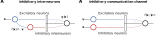
\includegraphics[trim=0cm 0cm 7.9cm 0cm,clip]{media/chapter_multi_compartment_lif/inhibitory_interneurons_overview.pdf}\hspace{0.4204cm}%
	\includegraphics[trim=0cm 0cm 7.9cm 0cm,clip]{media/chapter_multi_compartment_lif/inhibitory_interneurons.pdf}%
	{\phantomsubcaption\label{fig:inhibitory_interneurons_a}}%
	{\phantomsubcaption\label{fig:inhibitory_interneurons_b}}%
	\caption[Inhibitory interneurons and communication channels]{Inhibitory interneurons and communication channels.
	\textbf{(A)} To establish interneuron populations, we compute the identity function $f(x) = x$ in the purely excitatory projection onto the interneurons.
	The desired $\phi(\vec x)$ is then decoded from a virtual population encompassing both the inhibitory interneurons, and the excitatory pre-neurons.
	\textbf{(B)} Using this scheme, we can compute linear and nonlinear functions $\phi(x)$.
	Data for $100$ neurons per population with maximum firing rates between $50$ and $100\,\mathrm{Hz}$; weight matrices are determined by solving \cref{eqn:decode_nonneg} with $\sigma = 10$.
	The dotted line is the target $\phi(x)$, black line is the median decoded value over 1000 trials, shaded grey areas correspond to the 10th and 90th percentiles.
	Errors $E$ are the mean NRMSE with standard deviation.
	}
\end{figure}

\subsubsection{Inhibitory interneuons}
Connectivity patterns in biology do not suggest an arbitrary split of neural ensembles into excitatory and inhibitory neurons.
Instead, as we explained in Section~2.3.6, excitatory signals are often mediated through interneurons that provide local inhibition \citep[e.g.,][Chapter~2]{kandel2012principles}.
\citet{parisien2008solving} suggest a way to 
construct NEF networks with such inhibitory interneurons.

The techniques we discussed above can similarly be used to construct networks with inhibitory interneurons, albeit in a much simpler manner.
Recall that we can compute the identity function over purely excitatory connections (cf.~\Cref{fig:nonnegative_experiments}).
We can hence represent $\vec x$ in the interneurons using excitatory connection weights (cf.~\Cref{fig:inhibitory_interneurons_a}).
With this connection in place, the pre- and interneurons can be thought of as forming a \enquote{virtual pre-population} representing $\vec x$.
Using \cref{eqn:decode_nonneg} we can solve for excitatory weights $\vec w_i^+$ originating from the pre-population, and inhibitory weights $\vec w_i^-$ originating from the interneurons, that project onto the post-population while approximating a function $\phi(\vec x)$.

Although we decode from multiple pre-populations, we do not need to resort to an optimisation problem such as \cref{eqn:decode_current_additive}, where we decoded additive functions from multiple pre-populations.
This is possible because both pre-populations represent the same value.
Hence, we do not require a double integral, and we can compute nonlinear functions over $\vec x$.

As depicted in \Cref{fig:inhibitory_interneurons_b}, we can use this technique to approximate linear and nonlinear functions $\phi(\vec x)$; errors mostly stem from the pre- to interneuron connection.
Crucially, in contrast to the \enquote{Parisien transform}, we did not take any special precautions regarding the interneuron tuning curve distributions.
All populations use the \enquote{standard} tuning with uniform $x$-intercepts.
This is possible because we solve for weights directly in the current space.

\begin{figure}
	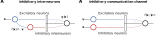
\includegraphics[trim=7.9cm 0cm 0cm 0cm,clip]{media/chapter_multi_compartment_lif/inhibitory_interneurons_overview.pdf}%
	\includegraphics[trim=7.9cm 0cm 0cm 0cm,clip]{media/chapter_multi_compartment_lif/inhibitory_interneurons.pdf}%
	{\phantomsubcaption\label{fig:inhibitory_comm_a}}%
	{\phantomsubcaption\label{fig:inhibitory_comm_b}}%
	\caption[Inhibitory communication channels]{Inhibitory communication channels.
	\textbf{(A)}~Inhibitory neurons can be used to form a communication channel, as long as there is some excitatory population that can provide a bias.
	\textbf{(B)}~Experiment demonstrating the use of this network setup as a communication channel.
	While the inhibitory connection is a good communication channel, nonlinear functions can only be computed with larger errors.
	All points are sampled from $(x, \nu) \in [-1, 1]^2$; the $\nu$-dimension is not depicted.
	See \Cref{fig:inhibitory_interneurons_b} for the network parameters and description of the depicted quantities.
	}
	\label{fig:inhibitory_comm}
\end{figure}

\subsubsection{Inhibitory communication channels}
Curiously, using the same techniques, we can also construct purely inhibitory communication channels---at least under the assumption that there is some separate excitatory pre-population that can be used as a bias source.
The lack of such an excitatory population is exactly what prevented us from computing functions across inhibitory connections in \Cref{fig:nonnegative_experiments}.

Assume that we have an inhibitory population representing $\vec x$, and another population representing some unrelated $\vec \nu$ (cf.~\Cref{fig:inhibitory_comm_a}).
Similar to \cref{eqn:decode_current_additive}, we minimise
\begin{align*}
	\min_{\vec w_i^+, \vec w_i^-}
	\frac{1}{\vol(\Xrepr)^2} \! \iint_{\Xrepr}
	\left(
		J_i\bigl(\langle \vec e_i, \phi(\vec x) \rangle\bigr)
		- \langle \vec w^-_i, -\vec a^-(\vec x) \rangle
		- \langle \vec w^+_i, \vec a^+(\vec \nu) \rangle
	\right)^2 \, d\vec x \, d\vec \nu + \sigma^2 \|\vec w_{i}^+\|_2^2 + \sigma^2 \|\vec w_{i}^-\|_2^2 \,,
\end{align*}
subject to $\vec w_{i}^+$, $\vec w_{i}^- > 0$.
Crucially, we ignore $\vec \nu$ in our target function; we solely use the pre-population to provide background activity but ignore its represented value.

Results of an experiment exploring this technique are depicted in \Cref{fig:inhibitory_comm_b}.
While computing the identity function---i.e., constructing a pure communication channel---works well, nonlinear functions can only be decoded with a considerable error, just as with purely excitatory connections channels (cf.~\Cref{fig:nonnegative_experiments}).
This is due to the standard NEF pre-population tuning curves not providing a good basis for nonnegative decoding of many nonmonotonic functions.
In principle, it should be possible to have pre-population tuning such that any nonnegative target current function can be nonnegatively decoded with an arbitrarily small error.
An example would be this Gaussian tuning curves similar to those depicted in \Cref{fig:bias_decoding_impact_c}.

Inhibitory networks similar to what we discussed here are explored in some more detail by \citet{tripp2016function}.
However, as with the Parisien transform, this prior work relies on specific tuning of the inhibitory neurons, as well as intrinsic biases.

\subsection{Subthreshold Relaxation}
\label{sec:nef_subthreshold}

\begin{figure}
	\includegraphics{media/chapter_multi_compartment_lif/subthreshold_illustration.pdf}%
	{\phantomsubcaption\label{fig:subthreshold_illustration_a}}%
	{\phantomsubcaption\label{fig:subthreshold_illustration_b}}%
	{\phantomsubcaption\label{fig:subthreshold_illustration_c}}%
	\caption[Illustration of the goal of subthreshold relaxation]{Illustration of the goal of subthreshold relaxation.
	\textbf{(A)} Most neurons act as rectifiers. Input currents below $J_\mathrm{th}$ (grey) are mapped onto zero.
	\textbf{(B)} Five randomly generated tuning curves with uniform $x$-intercepts and maximum firing rates between $50$ and $100$ spikes per second.
	\textbf{(C)} Using affine current-translation functions $J_i(\xi)$, these tuning curves are generated by comparably large negative currents. However, the magnitude of the currents below $J_\mathrm{th}$ (grey) has no effect on the output rate; in fact any current below $J_\mathrm{th}$ has the same effect on the firing rate of the neuron.
	}
\end{figure}

Most biological model neurons act as rectifiers.
That is, input currents below a certain, usually positive, threshold $J_\mathrm{th}$ do not result in any output activity.
In the case of our simplified LIF neuron model (cf.~Section~2.2.3), the threshold current $J_\mathrm{th}$ is \SI{1}{\nano\ampere} (\Cref{fig:subthreshold_illustration_a}).
We did not take this account in our above current-space optimisation schemes.

To the contrary, our current-based loss functions in \cref{eqn:decode_current,eqn:decode_nonneg} aim at \emph{precisely} evoking certain post-synaptic currents $J_\mathrm{tar}$.
Notably, the negative currents required by the affine current translation function $J_i(\xi)$ can be larger in magnitude than the positive currents (\Cref{fig:subthreshold_illustration_b,fig:subthreshold_illustration_c}).
This has not been an issue in NEF networks with intrinsic current-translation, as $J_i(\xi)$ takes care of appropriately scaling and offsetting the input currents.

However, in the context of our current-space optimisation schemes, a regularised least-squares optimisation problem can \enquote{prioritise} solving for exact (but irrelevant) subthreshold currents over solving for the (relevant) superthreshold currents.
This can lead to an increase in the superthreshold current-decoding error, and thus also increase the representation error in the post-population.
Additionally, as we will see below, dendritic nonlinearities impose asymptotic maximum and minimum post-synaptic currents.
Trying to solve for large negative currents may thus result in large connection weights.

One way to work around this issue is to clamp target currents $J_\mathrm{tar}$ that are substantially below the threshold to some constant.
For example, in the case of our simplified LIF neuron, we could clamp all negative target currents to a current of zero.
This way, the solver does not have to generate the afforementioned large negative subthreshold currents.
Still, this \enquote{clamping} approach requires the weight solver to \emph{precisely} solve for the desired target current although \emph{any} subthreshold current would do.

Conceptually, it would be better to \enquote{relax} the requirement to solve for $J_\mathrm{tar}$ as precisely as possible for subthreshold currents.
Instead, we could merely demand that subthreshold target currents are decoded as subthreshold currents, regardless of the magnitude.
If this constraint is violated, i.e., if the target current $J_\mathrm{tar}$ is below the threshold and the decoded current $J_\mathrm{dec}$ is above the threshold $J_\mathrm{th}$, we measure the distance to the threshold, and not the distance to $J_\mathrm{tar}$ as an error.
We formalise this as a superthreshold error function $\mathcal{E}$,
\begin{align}
\mathcal{E}(J_\mathrm{tar}, \, J_\mathrm{dec}) = \begin{cases}
0 & \text{if } J_\mathrm{tar} < J_\mathrm{th} \text{ and } J_\mathrm{dec} < J_\mathrm{th} \,,\\
J_\mathrm{dec} - J_\mathrm{th} & \text{if } J_\mathrm{tar} < J_\mathrm{th} \text{ and } J_\mathrm{dec} > J_\mathrm{th} \,,\\
J_\mathrm{dec} - J_\mathrm{tar} & \text{if } J_\mathrm{tar} \geq J_\mathrm{th} \,,\\
\end{cases}
\label{eqn:subthreshold_error}
\end{align}
and define a new current-space optimization problem akin to \cref{eqn:decode_nonneg}
\begin{align}
	\min_{\vec w_i^+, \vec w_i^-} 
	\frac{1}{\vol(\Xrepr)}
	\int_{\Xrepr} \mathcal{E}\left( 
		J_i(\langle \vec e_i, \phi(\vec x)\rangle),
		\langle \vec w_i^+, \vec a^+(\vec x) \rangle +
		\langle \vec w_i^-, -\vec a^-(\vec x) \rangle
	\right)^2 \, d\vec x
	+ \sigma^2 \| \vec w^+_i \|_\mathrm{2}^2
	+ \sigma^2 \| \vec w^-_i \|_\mathrm{2}^2\,.
\label{eqn:decode_current_subthreshold}
\end{align}

\subsubsection{Subthreshold relaxation as a quadratic program}
It is not immediately clear how to solve this optimisation problem.
While, it is always possible to resort to gradient descent, \cref{eqn:decode_current_subthreshold} can be solved more efficiently by rewriting the loss function in terms of a convex quadratic program (QP).
QPs are a generalisation of least-squares and defined as follows:
\begin{definition}[Quadratic Program]
\label{def:qp}
A \emph{quadratic program} (QP) is an optimisation problem of the form \citep[slightly simplified from][Section~4.4]{boyd2004convex}
\begin{align*}
	\text{minimize} &\quad
		\vec \omega^T \mat P \vec \omega + \mat q^T \vec \omega \\
	\text{subject to} &\quad
		\mat G \vec \omega \leq \vec h \,,
\end{align*}
where $\vec \omega \in \mathbb{R}^{n}$, $\mat G \in \mathbb{R}^{n \times n}$, $\vec p \in \mathbb{R}^{n}$, $\mat H \in \mathbb{R}^{\ell \times n}$, $\vec q \in \mathbb{R}^{\ell}$.
Here, $n$ is the number of variables and $\ell$ is the number of inequality constraints.
If $\vec x^T \mat P \vec x$ is a convex function (i.e., if $\mat P$ is positive definite).
%and the constraints $\mat G\vec x \leq \vec h$ form a convex polytope, then the QP is \emph{convex}.
\end{definition}

Convex quadratic programs can be solved in polynomial time \citep{kozlov1980polynomial}.
There are free and open-source software libraries, such as \enquote{cvxopt} \citep{vandenberghe2010cvxopt} and \enquote{OSQP}  \citep{stellato2020osqp} that solve such problems efficiently.
In our experiments we mostly rely on OSQP.%
\footnote{Some experiments were conducted before OSQP was published; we used cvxopt in those experiments. We did not observe any discernible difference in the solutions produced by the two libraries, but as a C library using more modern algorithms, OSQP is substantially faster than the older Python library cvxopt.}

To transform a discretised version of \cref{eqn:decode_current_subthreshold} into a quadratic program we split the sample points $\vec x_k$ according to whether they evoke super- or subthreshold currents.
Specifically, we arrange the pre-activities $\mat A$ and target currents $\mat J$ as follows:
\begin{align*}
	\mat{A}_\mathrm{sup} = (
		  \mat{A}^+_\mathrm{sup}, 
		- \mat{A}^-_\mathrm{sup})
		\in
		\mathbb{R}^{N_\mathrm{sup} \times (n^+ + n^-)} \,,
	&&
	\mat{J}_\mathrm{sup} \in \mathbb{R}^{N_\mathrm{sup}} \,,
	&&
	\mat{A}_\mathrm{sub} = (
		  \mat{A}^+_\mathrm{sub}, 
		- \mat{A}^-_\mathrm{sub})
		\in
		\mathbb{R}^{N_\mathrm{sub} \times (n^+ + n^-)} \,.
\end{align*}
Here, $N_\mathrm{sup}$, $N_\mathrm{sub}$ with $N = N_\mathrm{sup} + N_\mathrm{sup}$
are the number of samples with a super- and subthreshold target currents, and, as before, $n^+$ and $n^-$ correspond to the number of excitatory and inhibitory pre-neurons.
Using these matrices, \cref{eqn:decode_current_subthreshold} can be expressed as a QP by letting
\begingroup
\setlength\fboxsep{2pt}
\newcommand{\cA}{LightSkyBlue}
\newcommand{\cB}{Plum}
\newcommand{\cC}{Salmon}
\newcommand{\cD}{Khaki}
%\newcommand{\hlA}[1]{\colorbox{\cA}{\ensuremath{#1}}}
%\newcommand{\hlB}[1]{\colorbox{\cB}{\ensuremath{#1}}}
%\newcommand{\hlC}[1]{\colorbox{\cC}{\ensuremath{#1}}}
%\newcommand{\hlD}[1]{\colorbox{\cD}{\ensuremath{#1}}}
\newcommand{\hlA}[1]{{\ensuremath{#1}}}
\newcommand{\hlB}[1]{{\ensuremath{#1}}}
\newcommand{\hlC}[1]{{\ensuremath{#1}}}
\newcommand{\hlD}[1]{{\ensuremath{#1}}}
\begin{align}
	\mat P &= \begin{pmatrix}
		  \hlA{(\mat A_\mathrm{sup})^T \mat A_\mathrm{sup} + N \sigma^2 \mat I)}
		& 0 \\
		  0
		& \hlB{\mat I}
	\end{pmatrix} ,
	&
	\!\!\! \vec q &= \begin{pmatrix}
		\hlA{(\mat A_\mathrm{sup})^T \vec J_\mathrm{sup}} \\
	0
	\end{pmatrix} ,
	&
	\!\!\! \mat G &= \begin{pmatrix}
		\hlC{\mat A_\mathrm{sub}} & \hlB{\mat I} \\
		\hlD{-\mat I} & 0
	\end{pmatrix} ,
	&
	\!\!\! \vec h &= \begin{pmatrix}
		\hlC{\vec{J}_\mathrm{th}} \\
		\hlD{0}
	\end{pmatrix} .
	\label{eqn:decode_subthreshold_qp}
\end{align}
The number of variables is $n = n^+ + n^- + N_\mathrm{sub}$, and the number of inequality constraints is $\ell = N_\mathrm{sub} + n^+ + n^-$.
The parameter vector $\vec \omega \in \mathbb{R}^{n}$ can be split into the excitatory and inhibitory weights $\vec w_i^+ \in \mathbb{R}^{n^+}$, $\vec w_i^- \in \mathbb{R}^{n^-}$, as well as discardable slack variables $\vec s_i \in \mathbb{R}^{N_\mathrm{sub}}$.

The rationale behind \cref{eqn:decode_subthreshold_qp} is as follows.
The first line of $\mat P$ and $\vec q$
%(${\color{\cA}\blacksquare}$)
is the standard regularised least-squares problem obtained by expanding the superthreshold potion of \cref{eqn:decode_current_subthreshold} (cf.~\cite{boyd2004convex}, Section~4.4).
The first column and row of $\mat G$ and $\vec h$
%(${\color{\cC}\blacksquare}$)
add an inequality constraint that ensures that samples with subthreshold currents are decoded as subthreshold currents.
Violations of this constraint, i.e., case two of \cref{eqn:subthreshold_error}, are enabled by the slack variables $\vec s_i$ (second column of $\mat P$ and $\mat G$%
%; ${\color{\cB}\blacksquare}$
).
These slack variables correspond to the error $J_\mathrm{th} - J_\mathrm{tar}$, which is penalised accordingly in $\mat P$.
Finally, nonnegativity of the weights is ensured by the second row of $\mat G$ and $\vec h$%
% (${\color{\cD}\blacksquare}$)
. One can easily show that this QP is convex.
\endgroup

\begin{figure}
	\includegraphics{media/chapter_multi_compartment_lif/subthreshold_comparison.pdf}%
	{\phantomsubcaption\label{fig:subthreshold_comparison_a}}%
	{\phantomsubcaption\label{fig:subthreshold_comparison_b}}%
	{\phantomsubcaption\label{fig:subthreshold_comparison_c}}%
	{\phantomsubcaption\label{fig:subthreshold_comparison_d}}%
	\caption[Current decoding with and without subthreshold relaxation]{Current decoding with and without subthreshold relaxation in a setting with low regularisation ($\sigma = 0.31$) and few pre-neurons ($n = 50$).
	Values above each plot are the RMS of the superthreshold error ${\mathcal{E}}$ (eq.~\ref{eqn:subthreshold_error}).
	Subthreshold relaxation substantially reduces the decoding error.	
	}
	\label{fig:subthreshold_comparison}
\end{figure}

\subsubsection{Example: Individual post-neuron}
In \Cref{fig:subthreshold_comparison} we decode the post-synaptic currents for a single post neuron using NNLS, NNLS with clamped target currents, and subthreshold relaxation.
At least in this example, subthreshold relaxation substantially reduces the superthreshold decoding error.
In contrast, clamping the target currents has only a limited positive effect.
Notably, and particularly pronounced in the case of purely excitatory pre-neurons, the solution obtained with subthreshold relaxation is supported by more pre-neurons.
This is visible in \Cref{fig:subthreshold_comparison_c}, where subthreshold relaxation decodes a non-zero current for negative $\xi$, resulting in a smaller regularisation error (i.e., weight RMS of $0.8 \times 10^{-3}$ vs. $2 \times{10}^{-3}$).

\begin{figure}[t]
	\includegraphics{media/chapter_multi_compartment_lif/subthreshold_experiment.pdf}%
	{\phantomsubcaption\label{fig:subthreshold_experiment_a}}%
	{\phantomsubcaption\label{fig:subthreshold_experiment_b}}%
	{\phantomsubcaption\label{fig:subthreshold_experiment_c}}%
	\caption[Reduction in decoding error achieved with subthreshold relaxation]{Reduction in decoding error achieved with subthreshold relaxation compared to standard NNLS and clamping the target current.
	\textbf{(A)} Reduction in the decoded post-synaptic currents error relative to NNLS for different thresholds in the error measure $\mathcal{E}$.
	Each box plot over three functions, $100$ random networks, $11$ noise magnitudes, and $9$ random samplings of the noise ($N = 29\,700$); whiskers are the extrema, boxes the quartiles, orange line is the median, green dashed line the mean.
	\textbf{(B)}
	Same as \emph{(A)}, but for the post-population decoding error.
	\textbf{(C)} Same data as above, but over different pre-population noise magnitudes and for different functions $\phi(x)$ computed in the pre to post connection.
	Coloured lines show the median error (see \emph{(A, B)} for a legend); shaded areas are the 25\% and 75\% quartiles.
	}
	\label{fig:subthreshold_experiment}
\end{figure}

\subsubsection{Systematic experiment}
One issue with subthreshold relaxation is that avoiding to decode strongly negative currents can result in a narrower separation boundary between the threshold and the decoded current.
Hence, noise on the pre-activities is more likely to result in positive post-activity.
However, this may be compensated for by the smaller regularisation error, and hence higher robustness to noise as observed in the previous example.

\Cref{fig:subthreshold_experiment} depicts the results of a more systematic experiment.
We compute three polynomials in the connection between one hundred pre and post LIF rate neurons ($1\!\!:\!\!1$ excitatory to inhibitory ratio) with varying degree of Gaussian noise added to the pre-activities.
We select the regularisation factor $\sigma$ to minimize the error for the given amount of noise on a separate training set.
We furthermore vary the threshold $J_\mathrm{th}$ assumed in \cref{eqn:subthreshold_error}, to investigate the effect of moving $J_\mathrm{th}$ away from the true threshold.

As visible in \Cref{fig:subthreshold_experiment_a}, subthreshold relaxation reduces the current decoding error by about 50\% (median), largely independent of the assumed $J_\mathrm{th}$.
Clamping the currents leads to a reduction in error with a median of about 35\%, but, overall, the reduction in error is less consistent.
Improvements to the representation accuracy (\Cref{fig:subthreshold_experiment_b}) are less drastic, with the largest improvement for $J_\mathrm{th} = \SI{0.75}{\nano\ampere}$ with a median reduction in error of about 13\%.
This confirms our suspicion that setting $J_\mathrm{th}$ to the true threshold can be slightly detrimental.

This is further confirmed by the experiment in \Cref{fig:subthreshold_experiment_c} where we plot the post-population representation error over different pre-activity noise magnitudes.
For small amounts of noise subthreshold relaxation with $J_\mathrm{th} = \SI{1}{\nano\ampere}$ can lead to large improvements in the representation error; however, for larger noise magnitudes the overall benefit of subthreshold relaxation is smaller, with slightly reduced $J_\mathrm{th}$ performing the best.
We provide additional results from this experiment in Appendix C.2.

Keep in mind that LIF rate neurons are a worst-case scenario with respect to sensitivity to pre-activity noise injected near the threshold.
LIF rate neurons possess a very steep activity onset, where small changes in current lead to large fluctuations in activity.
This tends to be less of an issue with transient noise in spiking neural networks, which results in a smoother response curve (see our discussion below, as well as \cite{hunsberger2015spiking}).
We can thus expect that, in practice, the impact of subthreshold relaxation is somewhere between the values obtained for the current decoding and representation error.

\subsection{Extension Toward Dendritic Nonlinearities}
\label{sec:nef_nonlinear}

Up to this point we assumed current-based synapses.
As previously discussed in \Cref{sec:dendritic_computation_theory}, the defining property of current-based synapses is that the somatic current $J$ is linear in the synaptic weights $\vec w$ and the pre-synaptic activities $\vec a$, that is $a_i = G[J] = G[\langle \vec w, \vec a \rangle]$.
In contrast, we described neurons with nonlinear synapses as follows
\begin{align}
	a_i &=
	\mathscr{G} \bigl[
		g_i^1, \ldots, g_i^k
	\bigr] =
	\mathscr{G} \bigl[
		\langle \vec w_{i}^1, \vec a_1 \rangle,
		\ldots ,
		\langle \vec w_{i}^k, \vec a_k \rangle
	\bigr] \,.
\end{align}
Here, $k$ is the number of input channels, and the vector $\vec g_i = (g^1_i$, $\ldots$, $g^k_i)$ describes some abstract \enquote{channel state}.
Again, we assume that, on average, each channel state $g^j_i$ is linear in the weights and the ´activities $\vec a_j$ of the neurons connecting to the $j$th channel.
However, we do not make any assumption regarding the effect of $g^j_i$ on the somatic current $J$; more fundamentally, we do not assume that there exists an easily identifiable somatic current at all.

The lack of an identifiable somatic current makes it more challenging to integrate such neurons into the NEF.
The optimisation problems we discussed in this section relied on the current translation function $J_i(\xi)$ to enforce the normative tuning constraint $a_i(\vec x)$.
Of course, as mentioned above, we could resort to gradient descent to optimise \cref{eqn:dendritic_computation_optimisation}.
However, our current-based optimisation schemes work amiably well in that they allow us to quickly solve for globally optimal weights.
As we will see, it is still possible to perform global current-space optimisation for some multi-channel neurons.
Additionally, we can use the same ideas to iteratively solve for locally optimal weights in more complex multi-compartment neurons.

\begin{figure}
	\centering
	\includegraphics{media/chapter_multi_compartment_lif/two_compartment_response_curve.pdf}
	\caption[Neural response curve decomposition]{Neural response curve decomposition. \textbf{(A)} Illustration of the multivariate neuron response curve $\mathscr{G}(g_\mathrm{E}, g_\mathrm{I})$ for a two-compartment LIF neuron with excitatory and inhibitory conductance-based channels. \textbf{(B, C)} The chosen somatic nonlinearity $G$ and its inverse $G^{-1}$. \textbf{(D)} corresponding input-dependent nonlinearity $H$. The neuron does not fire in the hatched regions, that is, $G^{-1}$ is ill-defined.} 
	\label{fig:two_compartment_response_curve}
\end{figure}

To this end, the crucial idea is to mathematically reintroduce a \enquote{virtual} somatic current $J$ by decomposing $\mathscr{G}$ into the standard somatic nonlineartiy $G$ and a dendritic nonlinearity $H$.

\begin{definition}[Dendritic Nonlinearity]
\label{def:dendritic_nonlinearity}
Given a neural response curve $G$, the \emph{dendritic nonlinearity} $H(\vec g_i)$ of a multi-channel neuron with response curve $\mathscr{G}$ maps the input channel state $\vec g_i = (g^1_i, \ldots, g^k_i)$ onto an \emph{average}, time-independent somatic current $J$ such that
\begin{align}
		H\big(g^1_i, \ldots, g^k_i\big) = J
	\Leftrightarrow
		G\big[J\big] = \mathscr{G}\big[g^1_i, \ldots, g^k_i\big] 
	\Leftrightarrow
		\mathscr{G}\big[g^1_i, \ldots, g^k_i\big] = G\big[H(g^1_i, \ldots, g^k_i)\big] \,.
	\label{eqn:def_h}
\end{align}
\end{definition}
%This formalization does not constrain $G$ and $H$ beyond the above equivalence.
Optimally, $G$ is chosen such that $H$ is as simple as possible.
For example, if the neuron model is an extension to a LIF neuron, $G$ can be the standard LIF response curve.
In this case, $H$ translates the input into an \enquote{LIF-equivalent current}.
In the trivial case of the above current-based LIF neurons with excitatory and inhibitory inputs, we would obtain $H(J_\mathrm{E}, J_\mathrm{I}) = J_\mathrm{E} - J_\mathrm{I}$.

We use the dendritic nonlinearity $H$ to define a new current-space loss
\begin{align}
	E = \frac{1}{\vol(\Xrepr)} \int_{\Xrepr}
		\mathcal{E} \bigl(
			J_i(\langle \vec e_i, f(\vec x_k) \rangle),
			H(\langle \vec w^1_i, \vec a^k \rangle, \ldots, \langle \vec w^k_i, \vec a^k \rangle)
		\bigr)^2 \,\mathrm{dx} + \sigma^2 \sum_{j = 1}^\ell \| \vec w^j_i \|_2^2\,,
\label{eqn:decode_nonlinear_synapses}
\end{align}
where $\mathcal{E}$ is the superthreshold error defined in \cref{eqn:subthreshold_error}, $\vec a^j$ are the pre-activities connection, and weights $\vec w_i$ may be---depending on the input channel type---nonnegative.

We next show that it is possible to derive $H$, or at least a suitable surrogate model, in closed form for multi-compartment LIF neurons with conductance-based synapses.
If $H$ cannot be derived in closed form, we can sample $\mathscr{G}$ over varying synaptic states and, as depicted in \Cref{fig:two_compartment_response_curve}, compute $H$ indirectly by applying an inverse mapping $G^{-1}$ to the recorded data.

\section{A Family of Multi-Compartment LIF Neurons}
\label{sec:nlif}

The dendritic nonlinearity $H$ introduced in the last section maps some channel state $\vec g$ onto an average somatic current.
While this mapping can always be established numerically, expressing $H$ in closed form has the potential to simplify the optimisation problem in \cref{eqn:decode_nonlinear_synapses}.

In this section, we discuss a family of multi-compartment LIF neurons that we refer to as \enquote{$n$-LIF}.
These neuron models are based on the multi-compartment neurons that we reviewed in Section~2.1.4, and, as we discussed in the introduction of this chapter, were constructed with mathematical tractability in mind, rather than biological detail.
While it is not possible to derive an exact dendritic nonlinearity $H$ for these neurons, we derive a closed-form \enquote{surrogate} model of $H$ that can be fit to numerical data.
% TODO: Add reference \citep[cf.][Chapter~2]{gerstner2002spiking} above
%The idea is to preserve a single active leaky integrate-and-fire compartment, yet attach a passive dendritic tree as a somatic current source.
%% TODO: Check Chapter number
%In contrast to most other multi-compartment models, and in particular prior analyses to this end \citep[Chapter~5]{koch1999biophysics}, our dendritic tree model is rather simplistic.
%It neither accounts for propagation delays, nor short-term adaptation and dendritic spikes.
%However, incorporating this amount of biological detail into our model would make it impossible to find a close-form solution for $H$, and likely prevent us from meaningfully extending the NEF (cf.~Section~2.3.6).
% TODO: Move to the chapter introduction

\subsection{Mathematical Description of $n$-LIF Neurons}
\label{sec:nlif_description}

\begin{figure}
	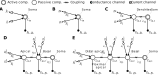
\includegraphics{media/chapter_multi_compartment_lif/multi_compartment_examples.pdf}%
	{\phantomsubcaption\label{fig:nlif_a}}%
	{\phantomsubcaption\label{fig:nlif_b}}%
	{\phantomsubcaption\label{fig:nlif_c}}%
	{\phantomsubcaption\label{fig:nlif_d}}%
	\caption[\enquote{Ball-and-stick} illustration of multi-compartment LIF neurons]{\enquote{Ball-and-stick} illustration of multi-compartment LIF neurons.
	Large circles correspond to compartments, small circles and rectangles to conductance- and current-based channels. Filled symbols indicate passive channels.
	\textbf{(A)} Standard LIF neuron with current-based inputs.
	\textbf{(B)} LIF neuron with conductance-based input channels.
	\textbf{(C)} Two-compartment LIF neuron with a separate dendritic compartment.
	\textbf{(D)} A three-compartment LIF neuron with distal and proximal dendritic compartments.}
	\label{fig:nlif}
\end{figure}

We define an $n$-LIF neuron as a connected graph of resistively coupled capacitive compartments.
Each neuron possesses exactly one active compartment with standard LIF dynamics, while the other compartments represent a passive dendritic tree.
Each compartment may hold any number of passive current- and conductance-based channels.
Channels are either constant (representing bias currents and leak channels), or receive external input (representing synapses).
Examples of such neurons are depicted in \Cref{fig:nlif} using a \enquote{ball-and-stick} representation.

As a point of reference, the expanded equivalent circuit diagram of the two-compartment LIF neuron with conductance-based synapses (\Cref{fig:nlif_c}) is depicted in \Cref{fig:two_comp_lif_circuit}.
This particular model has originally been described by \citet{vu1993mechanism} and was subsequently discussed by \citet{koch1999biophysics} and \citet{capaday2006direct}.
We discuss this model in more detail in the next section, and for now focus on $n$-LIF neurons in general.

\begin{figure}
	\includegraphics{media/chapter_multi_compartment_lif/neuron_model_trace_composite.pdf}%
	{\phantomsubcaption\label{fig:two_comp_lif_circuit}}
	{\phantomsubcaption\label{fig:two_comp_lif_trace}}
	\caption[Circuit and membrane potential trace of a two-compartment LIF neuron]{Circuit and membrane potential trace of a two-compartment LIF neuron.
	\textbf{(A)} Circuit diagram corresponding to the model in \Cref{fig:nlif_c}.
	\textbf{(B)} Membrane potential traces for both compartments for a small constant excitatory input.
	Notice how the explicit spike model in the somatic compartment (\emph{top}) influences the membrane potential of the dendritic compartment (\emph{bottom}).}
	\label{fig:two_comp_lif}
\end{figure}

\subsubsection{Superthreshold dynamics}
In contrast to the standard LIF model (cf.~Section~2.2.3), the active $n$-LIF compartment possess an explicit spike model.
% TODO: Add correct reference
As pointed out by \citet{capaday2006direct}, this is important in multi-compartment models, since the spike potential causes a substantial current to flow into the dendritic compartments (cf.~\Cref{fig:two_comp_lif_trace}).

More precisely, we model the superthreshold dynamics as follows.
Whenever the membrane potential \vMem surpasses the threshold $v_\mathrm{th}$, \vMem is clamped to a \enquote{spike potential} $v_\mathrm{spike}$ for a period $\tau_\mathrm{spike}$ and subsequently forced to $v_\mathrm{reset}$ for the refractory period $\tau_\mathrm{ref}$.
Unless specified otherwise, we use $\tau_\mathrm{spike} = \SI{1}{\milli\second}$ and $\tau_\mathrm{ref} = \SI{2}{\milli\second}$ in our models.

\subsubsection{Subthreshold dynamics}
The dynamics of the $i$th compartment are
\begin{align}
	C_\mathrm{m, i} \frac{d}{dt} v_i(t) &=
		\sum_{k=1}^{M_i} g_k^i(t) \bigl( E_k^i - v_i(t) \bigr) +
		\sum_{k=1}^{N_i} J_k^i(t) +
		\sum_{j=1}^{n} \bigl(v_j(t) - v_i(t)\bigr) c_{ij} \,,
\label{eqn:nlif_single_compartment}
\end{align}
where $C_\mathrm{m, i}$ is the membrane capacitance of the compartment, $M_i$ and $N_i$ are the number of conductance- and current-based channels, respectively, $g_{k}^i(t)$ is the momentary conductance of the $k$th conductance-channel with reversal potential $E_{k}^i$, and $J_{k}^i(t)$ is the current injected into the current-based channel $j$.
Finally, $c_{ij}$ is the coupling conductance between the $i$th and the $j$th compartment.
The adjacency matrix of coupling conductances $\mat C$ must be symmetric, and the connectivity graph encoded by $\mat C$ must have exactly one connected component (cf.~our discussion in Section~2.2.3).
%TODO: Correct reference
Some conductances $g_{k}^i(t)$ and currents $J_{k}^i(t)$ are constant, such as the static leak channels and bias currents.

\begin{table}
	\caption[Matrix representations of the neuron models in \Cref{fig:nlif}]{Matrix representations of the neuron models in \Cref{fig:nlif}. See text for a description.
	%All matrices are multiplied by the membrane capacitance $C_\mathrm{m}$ (assuming that $C_\mathrm{m}$ is the same across compartments).
	}
	\label{tbl:nlif_matrices}
	\small\sffamily\centering
	\begin{tabular}{c c c c c c}
		\toprule
		\multicolumn{1}{c}{\textbf{Model}} & $\vec{a}'$ & $\mat{A}'$ & $\vec{b}'$ & $\mat{B}'$ & $\mat L$ \\
		\midrule
		%\cmidrule{1-1}\cmidrule(l){2-6}
			\textbf{(A)}
			& $\displaystyle \begin{bmatrix} g_\mathrm{L} \end{bmatrix}$
			& $\displaystyle \begin{bmatrix} 0 & 0 \end{bmatrix}$
			& $\displaystyle \begin{bmatrix} g_\mathrm{L} E_\mathrm{L} \end{bmatrix}$
			& $\displaystyle \begin{bmatrix} 1 & -1 \end{bmatrix}$
			& $\displaystyle \begin{bmatrix} 0 \end{bmatrix}$\\[0.5cm]
			\textbf{(B)} 
			& $\displaystyle \begin{bmatrix} g_\mathrm{L} \end{bmatrix}$
			& $\displaystyle \begin{bmatrix} 1 & 1 \end{bmatrix}$
			& $\displaystyle \begin{bmatrix} g_\mathrm{L} E_\mathrm{L} \end{bmatrix}$
			& $\displaystyle \begin{bmatrix} E_\mathrm{E} & E_\mathrm{I} \end{bmatrix}$
			& $\displaystyle \begin{bmatrix} 0 \end{bmatrix}$ \\[0.5cm]
			\textbf{(C)} 
			& $\displaystyle \begin{bmatrix}
				g_\mathrm{L} \\ g_\mathrm{L}
			\end{bmatrix}$
			& $\displaystyle \begin{bmatrix} 0 & 0 \\
				1 & 1 \end{bmatrix}$
			& $\displaystyle \begin{bmatrix}
				g_\mathrm{L} E_\mathrm{L} \\
				g_\mathrm{L} E_\mathrm{L}
			\end{bmatrix}$
			& $\displaystyle \begin{bmatrix}
				0 & 0 \\
				E_\mathrm{E} & E_\mathrm{I}
			\end{bmatrix}$
			& $\displaystyle \begin{bmatrix} c_{12} & -c_{12} \\ -c_{12} & c_{12} \end{bmatrix}$ \\[0.5cm]
			\textbf{(D)} 
			& $\displaystyle \begin{bmatrix}
				g_\mathrm{L} \\
				g_\mathrm{L} \\
				g_\mathrm{L}
			\end{bmatrix}$
			& $\displaystyle \begin{bmatrix} 0 & 0 & 0 & 0\\
				0 & 0 & 1 & 1 \\
				1 & 1 & 0 & 0 \end{bmatrix}$
			& $\displaystyle \begin{bmatrix}
				g_\mathrm{L} E_\mathrm{L} \\
				g_\mathrm{L} E_\mathrm{L} \\
				g_\mathrm{L} E_\mathrm{L}
			\end{bmatrix}$
			& $\displaystyle \begin{bmatrix}
				0 & 0 & 0 & 0 \\
				0 & 0 & E_\mathrm{E} & E_\mathrm{I} \\
				E_\mathrm{E} & E_\mathrm{I} & 0 & 0 \\
			\end{bmatrix}$
			& $\displaystyle \begin{bmatrix} c_{12} & -c_{12} & 0 \\ -c_{12} & c_{12} + c_{23} & -c_{23} \\ 0 & -c_{23} & c_{23} \end{bmatrix}$ 			\\
		\bottomrule
	\end{tabular}
\end{table}

\subsubsection{Canonical matrix form}
We can rearrange \cref{eqn:nlif_single_compartment} to \emph{resemble} a canonical LTI system.%
\footnote{
Note that \cref{eqn:nlif_matrix} generally does \emph{not} describe a linear dynamical system (hence the emphasis on \enquote{resemble}).
There are two conditions under which this system is linear: either $\vec g(t)$ is constant, or there are no product terms between $\vec g(t)$ and $\vec v(t)$.
This is the case if the system has no conductance-based input channels and $\mat A'$ is zero.
}
Let $k$ be the number of non-static input channels, and $\vec g \in \mathbb{R}^k$ a vector representing the all input channel states, that is, all non-static conductances $g_{ij}$ and currents $J_{ij}$.
This channel state is generally linear in the synaptic weights and the pre-activities (cf.~\Cref{sec:nef_nonlinear}).
We have
\begin{align}
	\frac{d}{dt} \vec{C}_\mathrm{m} \circ \vec v(t)
	&= \mat A\big[\vec g(t)\big] \vec v(t) + \vec b\big[\vec g(t)\big]
	 = -\big[\mat L + \mathrm{diag}\big(\vec a' + \mat A' \vec g(t)\big)\big] \vec v(t) + \big[\vec b' + \mat B' \vec g(t)\big] \,.
	\label{eqn:nlif_matrix}
\end{align}
Here, $\vec{C}_\mathrm{m} \in \mathbb{R}^n$ is a vector of membrane capacitances and \enquote{$\circ$} is elementwise multiplication.
Furthermore, $\mat A[\vec g(t)] \in \mathbb{R}^{n \times n}$ is a \enquote{voltage feedback matrix}, and $\vec b[\vec g(t)] \in \mathbb{R}^n$ describes the input to the system.
We further decompose $\mat A$ and $\vec b$ into input-independent -dependent terms.
The Laplacian $\mat L \in \mathbb{R}^{n \times n}$ and the vectors $\vec a' \in \mathbb{R}^n$, $\vec b' \in \mathbb{R}^n$ describe the input-independent portions of the system, whereas the matrices $\mat A' \in \mathbb{R}^{n \times k}$ and $\mat B' \in \mathbb{R}^{n \times k}$ describe its input-dependent parts.

More specifically, the graph Laplacian $\mat L$ is the difference between the weighted degree matrix and the adjacency matrix, and, in our case, is given as $\mat L = \diag(\mat C \mat I) - \mat C$.
The vector $\vec a'$ consists of the sums of all conductances of all static conductance-based channels (such as the leak channel conductance) and $\vec b'$ contains the sums of the static channel conductances multiplied by their reversal potential.
The matrix $\mat A'$ contains one-entries for input-variables influencing a conductance-based channel in the corresponding compartment.
In turn, $\mat B'$ contains a \enquote{one} for each variable influencing a current-based channel in the corresponding compartment, and the reversal potential for conductance-based channels influenced by a variable in a compartment.
Examples of these matrices for the $n$-LIF neuron models depicted in \Cref{fig:nlif} are given in \Cref{tbl:nlif_matrices}.

\subsection{Deriving a Surrogate Model of the Dendritic Nonlinearity $H$}

As defined above (cf.~\Cref{def:dendritic_nonlinearity}), the dendritic nonlinearity $H$ maps a synaptic state $\vec g$ onto the synaptic current $J$ such that $G[J] = \mathscr{G}[\vec g]$, where $G[J]$ is a standard single-channel response curve and $\mathscr{G}[\vec g]$ is the response curve of the multi-channel neuron.
If, for example, $G[J]$ is the LIF response curve, then $H$ maps $\vec g$ into an \enquote{LIF-equivalent} current.

Trivial cases aside, it is generally not possible to provide $H$ in closed form for $n$-LIF neurons.
This is due to the nonlinear interaction between the membrane potential and conductance-based input channels, as well as the influence of the nonlinear superthreshold dynamics on the dendritic compartments.
Still, we can derive a parametrised \enquote{surrogate model} that approximates $H$ well and that we can fit to empirical data.

\subsubsection{Subthreshold current}
As a first step toward this model, consider the case where the neuron model is purely in its subthreshold regime.
Without loss of generality, assume that the compartment with index $i = 1$ is the somatic compartment.
Furthermore, assume that this compartment possesses a leak channel with conductance $g_\mathrm{L}$ and reversal potential $E_\mathrm{L}$.
The current $H(\vec g; t)$ flowing into the somatic compartment at time $t$ for constant $\vec g$ is the differential of $v_1$ divided by the membrane capacitance, that is
\begin{align}
	H(\vec g; t) = \big(\mat A[\vec g] \vec v(t) + \vec b[\vec g] \big)_1 \,.
	\label{eqn:nlif_sub_momentary}
\end{align}
To obtain an LIF-equivalent current, we must further subtract the leak current $g_\mathrm{L} \big( E_\mathrm{L} - v_1(t) \big)$; this current is already accounted for in the LIF response curve $G[J]$.%
\footnote{
Of course, $H$ depends on the specific choice of $G[J]$.
For example, if we used the response curve for an non-leaky IF-neuron instead, we would not have to subtract the leak current.
More specifically, in the next section, we discuss using a rectified linear unit instead of the LIF response curve.
Also note that, in practice, these details are not too critical.
As we discuss below, we propose use a parametrised version of $H$ that is fit to numerical measurements of $J$; this process naturally compensates for missing offsets.
}

\begin{figure}[p]
	\centering
	\includegraphics{media/chapter_multi_compartment_lif/average_som_pot.pdf}%
	{\phantomsubcaption\label{fig:avg_vsom_a}}%
	{\phantomsubcaption\label{fig:avg_vsom_b}}%
	\caption[Mean somatic membrane potential over the neuron output rate]{Mean somatic membrane potential $\vSom$ over the output rate for a current-based LIF neuron. Lines correspond to the average potential for different pre-synaptic spike rates.
	Mean post-synaptic currents are fixed in individual trials, so the spike rate purely corresponds to the amount of noise.
	Data over 128 random Poisson spike-trains per 1000 individual mean post-synaptic currents.
	Synaptic filter time constant is $5\,\mathrm{ms}$. Shaded areas correspond to 25/75\% percentiles, lines to the mean. \textbf{(A)} Average membrane potential excluding the refractory and spike period. Dotted line is a  linear model that takes the relative length of the spike and refractory phase into account. \textbf{(B)} Average membrane potential including the refractory and spike period.}
	\label{fig:avg_vsom}
\end{figure}

\begin{table}[p]
	\caption[Reduced matrix representations of the neuron models in \Cref{fig:nlif}]{Reduced matrix representations of the multi-compartment neuron models in \Cref{fig:nlif}.
	The somatic compartment is disconnected from the remaining neuron model.
	Connections to the somatic compartment are replaced by a static conductance-based channel with reversal potential $\vSom$. The voltage difference between $\vSom$ and the equilibrium potential of the new model is proportional to the current flowing into the somatic compartment.
	}
	\label{tbl:nlif_matrices_reduced}
	\small\sffamily\centering
	\begin{tabular}{c c c c c c c}
		\toprule
		\multicolumn{1}{c}{\textbf{Model}\!\!} & $\vec{\tilde a}'$ & $\mat{\tilde A}'$ & $\vec{\tilde b}'$ & $\mat{\tilde B}'$ & $\mat{\tilde L}$ & $\vec{\tilde c}$\\
		\midrule
			\textbf{(A)}
			& $\displaystyle \begin{bmatrix} 1 \end{bmatrix}$
			& $\displaystyle \begin{bmatrix} 0 & 0 \end{bmatrix}$
			& $\displaystyle \begin{bmatrix} g_\mathrm{L} ( E_\mathrm{L} - \vSom ) + \vSom \end{bmatrix}$
			& $\displaystyle \begin{bmatrix} 1 & -1 \end{bmatrix}$
			& $\displaystyle \begin{bmatrix} 0 \end{bmatrix}$
			& $\displaystyle \begin{bmatrix} 1 \end{bmatrix}$\\[0.5cm]
			\textbf{(B)}
			& $\displaystyle \begin{bmatrix} 1 \end{bmatrix}$
			& $\displaystyle \begin{bmatrix} 0 & 0 \end{bmatrix}$
			& $\displaystyle \begin{bmatrix} g_\mathrm{L} ( E_\mathrm{L} - \vSom ) + \vSom \end{bmatrix}$
			& $\displaystyle \begin{bmatrix} E_\mathrm{E} - \vSom & E_\mathrm{I} - \vSom \end{bmatrix}$
			& $\displaystyle \begin{bmatrix} 0 \end{bmatrix}$
			& $\displaystyle \begin{bmatrix} 1 \end{bmatrix}$\\[0.5cm]
			\textbf{(C)}
			& $\displaystyle \begin{bmatrix}
				1 \\
				g_\mathrm{L} + c_\mathrm{12}
			\end{bmatrix}$
			& $\displaystyle \begin{bmatrix}
				0 & 0 \\
				1 & 1 \end{bmatrix}$
			& $\displaystyle \begin{bmatrix}
				g_\mathrm{L} ( E_\mathrm{L} - \vSom ) + \vSom \\
				g_\mathrm{L} E_\mathrm{L} + c_{12} \vSom
			\end{bmatrix}$
			& $\displaystyle \begin{bmatrix}
				0 & 0 \\
				E_\mathrm{E} & E_\mathrm{I}
			\end{bmatrix}$
			& $\displaystyle \begin{bmatrix} 0 & 0 \\ 0 & 0 \end{bmatrix}$
			& $\displaystyle \begin{bmatrix} 1 \\ c_{12} \end{bmatrix}$\\[0.5cm]
			\textbf{(D)} 
			& $\displaystyle \begin{bmatrix}
				1 \\
				g_\mathrm{L} + c_\mathrm{12}\\
				g_\mathrm{L}
			\end{bmatrix}$
			& $\displaystyle \begin{bmatrix}
				0 & 0 & 0 & 0 \\
				0 & 0 & 1 & 1 \\
				1 & 1 & 0 & 0 \end{bmatrix}$
			& $\displaystyle \begin{bmatrix}
				g_\mathrm{L} ( E_\mathrm{L} - \vSom ) + \vSom \\
				g_\mathrm{L} E_\mathrm{L} + c_{12} \vSom \\
				g_\mathrm{L} E_\mathrm{L}
			\end{bmatrix}$
			& $\displaystyle \begin{bmatrix}
				0 & 0 & 0 & 0 \\
				0 & 0 & E_\mathrm{E} & E_\mathrm{I} \\
				E_\mathrm{E} & E_\mathrm{I} & 0 & 0 \\
			\end{bmatrix}$
			& $\displaystyle \begin{bmatrix}
				0 & 0 & 0 \\
				0 & c_{23} & -c_{23} \\
				0 & -c_{23} & c_{23} \end{bmatrix}$
			& $\displaystyle \begin{bmatrix} 1 \\ c_{12} \\ 0 \end{bmatrix}$\\
		\bottomrule
	\end{tabular}
\end{table}

\subsubsection{Average superthreshold somatic potential}
For or the purpose of building networks of spiking neurons, we are primarily interested in the superthreshold regime.
Unfortunately, as mentioned above, the nonlinear superthreshold dynamics are notoriously difficult to analyse.

We work around this by exploiting that $n$-LIF neurons are tonically spiking (cf.~Section~2.2.1).
That is, the somatic compartment oscillates between the reset and threshold potential with a fixed frequency (cf.~Figure~2.20).
%TODO Fix references
We may thus assume that the somatic membrane potential is effectively clamped to some value $\vSom$ between reset and threshold potential; we discuss this in more detail in \citet{stockel2017point}.
%TODO Use "clip" instead of "clamp" in the subthreshold description

As is depicted in \Cref{fig:avg_vsom}, this assumption is reasonable for a wide range of output rates, as long as we ignore the spike and refractory period.
This latter simplification is justified, since due to clamping, the current flowing into the somatic compartment during these periods has no direct influence on the output rate of the neuron.
Of course, in multi-compartment models, there is the smaller, indirect effect of the somatic membrane potential influencing the state of the dendritic compartments, but we ignore this for now.

\pagebreak

\subsubsection{Average somatic current}
To estimate the average current flowing into the somatic compartment, we replace the system from \cref{eqn:nlif_matrix} with a reduced system with vectors and matrices $\vec{\tilde a}'$, $\vec{\tilde b}'$, $\mat{\tilde A}'$, $\mat{\tilde B}'$, and $\mat{\tilde L}'$.
These matrices describe a dynamical system of the form%
\footnote{
We ignore the membrane capacitances $C_\mathrm{m, i}$ in both \cref{eqn:nlif_matrix_reduced} and \cref{eqn:nlif_eq}.
The membrane capacitances solely influence the time-constants with which the system converges to the equilibrium, but not the equilibrium point itself.
To see this, remember that the membrane capacitances effectively divide the $i$th row of $\mat A[\vec g]$ and $\vec b[\vec g]$ by a constant vector $C_\mathrm{m, i}$. We can write this as a matrix-multiplication with a diagonal matrix and obtain
\begin{align*}
	\bigl(\diag(\vec C_\mathrm{m})^{-1} \mat A[\vec g]\bigr)^{-1} \bigl(\diag(\vec C_\mathrm{m})^{-1} \vec b[\vec g]\bigr) = \mat A[\vec g]^{-1} \diag(\vec C_\mathrm{m}) \diag(\vec C_\mathrm{m})^{-1} \vec b[\vec g] = \mat A[\vec g]^{-1} \vec b[\vec g] \,.
\end{align*}
In general, the system is invariant to scaling the rows of $\mat A[\vec g]$ and $\vec b[\vec g]$; there are $n$ superfluous degrees of freedom.
}
\begin{align}
	\frac{d}{dt} \vec{\tilde v}(t)
	&= \mat{\tilde A}\big[\vec g(t)\big] \vec{\tilde v}(t) + \vec{\tilde b}\big[\vec g(t)\big]
	 = -\big[\mat{\tilde L} + \mathrm{diag}\big(\vec{\tilde a'} + \mat{\tilde A'} \vec g(t)\big)\big] \vec v(t) + \big[\vec{\tilde b}' + \mat{\tilde B}' \vec g(t)\big] \,.
	\label{eqn:nlif_matrix_reduced}
\end{align}
For constant $\vec g$, this system is linear and converges to an equilibrium state $\vec {\tilde v}^\mathrm{eq}$
\begin{align}
	\vec{\tilde v}(t)
	=
	  \vec{\tilde v}^\mathrm{eq}
	+ \exp\bigl(
		-\mat{\tilde A}[\vec g] t
	  \bigr) \bigl(
	    \vec{\tilde v}(0) - \vec{\tilde v}^\mathrm{eq}
	  \bigr) \,,
	\quad\quad \text{where} \quad \vec{\tilde v}^\mathrm{eq} &= -{\mat{\tilde A}}[\vec g]^{-1} \vec{\tilde b}[\vec g] \,.
	\label{eqn:nlif_eq}
\end{align}
The reduced system is constructed such that, for non-somatic compartments, the equilibrium potential $\vec{\tilde v}^\mathrm{eq}$ converges to the voltage that we would obtain if the somatic compartment were clamped to \vSom. In the somatic compartment itself, the voltage difference $\tilde v^\mathrm{eq}_1 - \vSom$ is proportional to the current flowing into the compartment.
Given a vector $\vec{\tilde c}$ of somatic coupling conductances with $\tilde c_1 = 1$, the average current flowing into the soma is thus
\begin{align}
	H(\vec g) &= \lim_{T \to \infty} \frac{1}T \int_{0}^T H(\vec g; t) \,dt \approx \sum_{i = 1}^n \tilde c_i (\tilde v^\mathrm{eq}_i - \vSom) \,,
	\label{eqn:h_model}
\end{align}
To derive the reduced system, we assume that the somatic compartment is clamped to $\vSom$.
This is accomplished by setting the first column and row of $\mat{\tilde L}$ to zero and replacing connections to the somatic compartment with a static conductance-based channel with reversal potential $\vSom$ and conductance $c_{1, i}$.
In the somatic compartment itself, all conductance-based channels are replaced by current-based channels weighted by the difference between $\vSom$ and the channel reversal potential (cf.~\cite{stockel2017point}); furthermore, we let $(\vec {\tilde a}')_1 = 1$ and add $\vSom$ to $(\vec {\tilde b'})_1$.
We provide examples of reduced systems in \Cref{tbl:nlif_matrices_reduced}.

\subsubsection{Model parameters}
\Cref{eqn:nlif_eq} is the result of major simplifications and as such unlikely to be accurate.
Specifically, we assumed that the somatic compartment is effectively clamped to a constant potential $\vSom$, that $\vec g$ is constant, and that spike generation has no effect on the dendritic compartments.
These assumptions are readily violated in practice.
The average somatic potential $\vSom$ depends on the pre-synaptic noise-level (cf.~\Cref{fig:avg_vsom}), the input $\vec g$ is seldom constant, and spike generation affects the dendritic membrane potentials (cf.~\Cref{fig:two_comp_lif_trace}).

Thus, equation~(\ref{eqn:nlif_eq}) is better interpreted as a \enquote{template} for the overall mathematical shape of the dendritic nonlinearity.
That is, to at least partially compensate for the imprecisions in our derivation, we declare $\vec{\tilde a}'$, $\vec{\tilde b}'$, as well as the non-zero entries in $\mat{\tilde A}'$, $\mat{\tilde B}'$ to be free parameters.
Keeping the graph Laplacian $\mat{\tilde L}$ and the zeros in $\mat{\tilde A'}$, $\mat{\tilde B'}$ fixed implies that we assume that the connectivity graph accurately describes the electrical network of the neuron.

%Note that this parametrisation is not minimal, in the sense that it does not have the least possible number of degrees of freedom.

The model parameters can be initialised with the original model and fit to direct numerical measurements of the somatic current $J$, or, alternatively, currents reconstructed from the neural activity, i.e., $J = G^{-1}[\mathscr{G}(\vec g)]$.
The calibration samples should be obtained from a setting that resembles the network context in which the neuron is used.
For example, the pre-synaptic noise level should match what the neuron would be exposed to in the network.

We discuss methods for determining the model parameters, and test the quality of $H$ in the following sections.
However, before we do so, we explicitly derive $H$ for a few special cases and analyse this dendritic nonlinearity model from a more theoretical perspective.


\subsection{Some Worked Examples}
\label{sec:nlif_examples}

The above framework is well suited for algorithmically deriving the dendritic nonlinearity model $H$ for arbitrary $n$-LIF neurons.
Unfortunately, it may be less intuitive when manually analysing these models.
%We can easily construct the corresponding model matrices and predict the somatic current for a given input configuration.
Hence, we find it useful to at least provide the expanded dendritic nonlinearity $H$ for the four models depicted in \Cref{fig:nlif}.

\subsubsection{Single-compartment LIF neuron with current-based input}
Expanding \cref{eqn:h_model} for the model depicted in \Cref{fig:nlif_a} using \Cref{tbl:nlif_matrices_reduced} yields 
\begin{align*}
	H(J_\mathrm{E}, J_\mathrm{I}) = J_\mathrm{E} - J_\mathrm{E} + g_\mathrm{L}(E_\mathrm{L} - \vSom) \,.
\end{align*}
This function is visualised in \Cref{fig:dendritic_nonlinearity_comparison_a}. To obtain the LIF-equivalent current we subtract the leak current, as mentioned above.
Using the fully parameterised version of the equations, and renaming the parameters for better readability, we obtain the following affine model:
\begin{align*}
	H(J_\mathrm{E}, J_\mathrm{I}) &= \tilde b'_1 + \tilde B'_{1, 1} J_\mathrm{E} + \tilde B'_{1, 2} J_\mathrm{I} = b_0 + b_1 J_\mathrm{E} + b_2 J_\mathrm{I} \,.
\end{align*}

\begin{figure}
	\includegraphics{media/chapter_multi_compartment_lif/dendritic_nonlinearity_comparison.pdf}%
	{\phantomsubcaption\label{fig:dendritic_nonlinearity_comparison_a}}%
	{\phantomsubcaption\label{fig:dendritic_nonlinearity_comparison_b}}%
	{\phantomsubcaption\label{fig:dendritic_nonlinearity_comparison_c}}%
	{\phantomsubcaption\label{fig:dendritic_nonlinearity_comparison_d}}%
	\caption[Dendritic nonlinearity models $H$ for different $n$-LIF neurons]{Dendritic nonlinearity models $H$ for the $n$-LIF neurons depicted in \Cref{fig:nlif}. Hatched regions correspond to subthreshold currents. Limits were chosen such that the spike onset is approximately on the diagonal of each plot.
	Parameters shared between all models: $g_\mathrm{L} = \SI{50}{\nano\siemens}$, $C_\mathrm{m} = \SI{1}{\nano\farad}$, $E_\mathrm{L} = \SI{-65}{\milli\volt}$, $E_\mathrm{E} = \SI{20}{\milli\volt}$, $E_\mathrm{I} = \SI{-75}{\milli\volt}$, $\vSom = \SI{-57.5}{\milli\volt}$.
	\textbf{(A, B)} Single-compartment neurons with current- and conductance-based synapses. Apart from scaling, the two models are equivalent.
	\textbf{(C)}~Two-compartment LIF neuron with $c_\mathrm{12} = \SI{30}{\nano\siemens}$. The contour lines are still straight lines but no longer parallel due to shunting.
	\textbf{(D)} Slice through the response curve of a three-compartment LIF neuron with $c_\mathrm{12} = \SI{40}{\nano\siemens}$, $c_\mathrm{23} = \SI{100}{\nano\siemens}$. The inputs $g_E^2 = \SI{95}{\nano\siemens}$ and $g_I^1 = \SI{20}{\nano\siemens}$ are kept constant. In contrast to the two-compartment neuron, the contour-lines are curved.
	}
\end{figure}


\subsubsection{Single-compartment LIF neuron with conductance-based input}
For \Cref{fig:nlif_b} we obtain
\begin{align*}
	H(g_\mathrm{E}, g_\mathrm{I}) = g_\mathrm{E} (E_\mathrm{E} - \vSom) + g_\mathrm{I} (E_\mathrm{I} - \vSom) + g_\mathrm{L}(E_\mathrm{L} - \vSom) \,.
\end{align*}
This function is illustrated in \Cref{fig:dendritic_nonlinearity_comparison_b}.
The fully parameterised version of the model is
\begin{align*}
	H(g_\mathrm{E}, g_\mathrm{I}) &= \tilde b'_1 + \tilde B'_{1, 1} g_\mathrm{E} + \tilde B'_{1, 2} g_\mathrm{I} = b_0 + b_1 g_\mathrm{E} + b_2 g_\mathrm{I} \,.
\end{align*}
This is the equivalent to the current-based neuron model.

Crucially, this is not just an artefact of our modelling framework, but indeed captures the behaviour of spiking neuron simulations well.
We discuss this in more detail in \citet{stockel2017point}.
Independent experiments by \citet{kiselev2020approximating} further support this observation.
Hence, single-compartment LIF neurons with conductance-based synapses are rather uninteresting from a computational perspective.

\subsubsection{Two-compartment LIF neuron}
For the model depicted in \Cref{fig:nlif_b} we have
\begin{align}
	H(g_\mathrm{E}, g_\mathrm{I}) = c_{12} \left(\frac{\vSom c_\mathrm{12} + E_\mathrm{L} g_\mathrm{L} + E_\mathrm{E} g_\mathrm{E} + E_\mathrm{I} g_\mathrm{I}}{c_\mathrm{12} + g_\mathrm{L} + g_\mathrm{E} + g_\mathrm{I}} - \vSom \right) + g_\mathrm{L}(E_\mathrm{L} - \vSom) \,.
	\label{eqn:two_comp_lif_natural}
\end{align}
Interestingly, in the limit of increasing the coupling conductance $c_{12}$ to infinity we obtain
\begin{align*}
	\lim_{c_{12} \to \infty} H(g_\mathrm{E}, g_\mathrm{I}) &= 
		E_\mathrm{E} g_\mathrm{E} + E_\mathrm{I} g_\mathrm{I} + 2 g_\mathrm{L} (E_\mathrm{L} - \vSom) - \vSom (g_\mathrm{E} + g_\mathrm{I}) \,.
\end{align*}
that is, the two-compartment model reduces to an affine function if the two compartments are tightly coupled.
The fully parameterised version of the model is given as
\begin{align*}
	H(g_\mathrm{E}, g_\mathrm{I}) =
		c_{12} \left(\frac{
			\tilde b'_2 + \tilde B'_{2, 1} g_\mathrm{E} + \tilde B'_{2, 2} g_\mathrm{I}
		}{
			\tilde a'_2 + \tilde A'_{2, 1} g_\mathrm{E} + \tilde A'_{2, 2} g_\mathrm{I}
		} - \vSom \right) + b'_1 \,.
\end{align*}
An example of $H$ is depicted in \Cref{fig:dendritic_nonlinearity_comparison_c}.
Taking into account that the inhibitory channel should reduce the total current, we can rewrite this as a rational function and identify the maximum excitatory and inhibitory currents that can be generated by this model
\begin{align}
	H(g_\mathrm{E}, g_\mathrm{I}) &=
		\frac{
	        b_0 + b_1 g_\mathrm{E} - b_2 g_\mathrm{I}
        }{
	        a_0 + a_1 g_\mathrm{E} + a_2 g_\mathrm{I}
        } \,,
%    & \text{where } a_0 > 0 \text{ and } a_1, a_2 \geq 0 \,.
	& \lim_{g_\mathrm{E} \to \infty} H(g_\mathrm{E}, g_\mathrm{I}) &= \frac{b_1}{a_1} \,,
	& \lim_{g_\mathrm{I} \to \infty} H(g_\mathrm{E}, g_\mathrm{I}) &= -\frac{b_2}{a_2} \,,
	\label{eqn:two_comp_lif}
\end{align}
where $a_0 > 0$ and the other $a_1$, $a_2$, $b_0$, $b_1$, $b_2 \geq 0$.

\subsubsection{Three-compartment LIF neuron}
For models with more than two compartments, the dendritic nonlinearity model becomes rather unwieldy.
For the neuron model depicted in \Cref{fig:nlif_d}, the dendritic nonlinearity $H(g_\mathrm{E}^1, g_\mathrm{I}^1, g_\mathrm{E}^2, g_\mathrm{I}^2)$ is equal to:
\begin{align}
	\begin{aligned}
	 H = &~
		c_{12} \Bigl(
				\bigl[
					\hphantom{+} \; (
					  E_\mathrm{L} g_\mathrm{E}^1
					+ E_\mathrm{L} g_\mathrm{I}^1
					+ E_\mathrm{E} g_\mathrm{E}^2
					+ E_\mathrm{I} g_\mathrm{I}^2
					+ \vSom  c_\mathrm{12}
					+ 2 E_\mathrm{L} c_{23} 
					) g_\mathrm{L}\\
	&~\hspace{0.7cm} \;
					  + (
					    E_\mathrm{E} g_\mathrm{E}^1
					  + E_\mathrm{I} g_\mathrm{I}^1
					  + E_\mathrm{E} g_\mathrm{E}^2
					  + E_\mathrm{I} g_\mathrm{I}^2
					  \! + \! \vSom c_\mathrm{12}) c_{23}
                      + (g_\mathrm{E}^1 + g_\mathrm{I}^1)
					  (E_\mathrm{E} g_\mathrm{E}^2 + E_\mathrm{I} g_\mathrm{I}^2 + c_{12} \vSom) + g_\mathrm{L}^2 E_\mathrm{L}
				\bigr] \\
	&~\hspace{0.7cm}
				\bigl[
					\hphantom{+} \; (
					g_\mathrm{E}^1 +
					g_\mathrm{I}^1 +
					g_\mathrm{E}^2 +
					g_\mathrm{I}^2 +
					c_{12} +
					2 c_{23}) g_\mathrm{L} \\
	&~\hspace{0.7cm} \;
				  + (g_\mathrm{E}^1 + g_\mathrm{I}^1 + g_\mathrm{E}^2 + g_\mathrm{I}^2 \! + \! c_\mathrm{12}) c_{23}
				+ (g_\mathrm{E}^1 + g_\mathrm{I}^1) (g_\mathrm{E}^2 + g_\mathrm{I}^2 + c_{12}) + g_\mathrm{L}^2
			\bigr]^{-1}
			\! - \vSom
		\Bigr) \! + \! g_\mathrm{L}(E_\mathrm{L} \! - \! \vSom) \,.
	\end{aligned}
	\label{eqn:three_comp_lif_long}
\end{align}
A slice of this function is depicted in \Cref{fig:dendritic_nonlinearity_comparison_d}.
Since it might not be immediately apparent, note that for $c_{23} \to 0$ the fraction in the above equation reduces to
\begin{align*}
		\frac{
			(g_\mathrm{L} + g_\mathrm{E}^1 + g_\mathrm{I}^1) (E_\mathrm{E} g_\mathrm{E}^2 + E_\mathrm{I} g_\mathrm{I}^2 + E_\mathrm{L} g_\mathrm{L} + c_\mathrm{12} \vSom)
		}{
			(g_\mathrm{L} + g_\mathrm{E}^1 + g_\mathrm{I}^1)
			(g_\mathrm{L} + c_{12} + g_\mathrm{E}^2 + g_\mathrm{I}^2)
		}
	 =
	 		\frac{
				E_\mathrm{E} g_\mathrm{E}^2 + E_\mathrm{I} g_\mathrm{I}^2 + E_\mathrm{L} g_\mathrm{L} + c_\mathrm{12} \vSom
	 		}{
				g_\mathrm{L} + c_{12} + g_\mathrm{E}^2 + g_\mathrm{I}^2
	 		} \,,
\end{align*}
%and for $c_{23} \to \infty$ we obtain
%\begin{align*}
%	 		\frac{
%				E_\mathrm{E} (g_\mathrm{E}^1 + g_\mathrm{E}^2) + E_\mathrm{I} (g_\mathrm{I}^1 + g_\mathrm{I}^2) + E_\mathrm{L} g_\mathrm{L} + c_\mathrm{12} \vSom
%	 		}{
%				g_\mathrm{L} + c_{12} + g_\mathrm{E}^1 + g_\mathrm{E}^2 + g_\mathrm{I}^1 + g_\mathrm{I}^2
%	 		} \,.
%\end{align*}
that is, the neuron reduces to the two-compartment neuron. The same is true for $c_\mathrm{23} \to \infty$.

There is little room for simplifying \cref{eqn:three_comp_lif_long} further.
However, notice that the numerator and denominator only contain products-terms between the input channels of different compartments.
We can thus write $H$ as
\begin{align}
	H(g_\mathrm{E}^1, g_\mathrm{I}^1, g_\mathrm{E}^2, g_\mathrm{I}^2) =
		\frac{
	        b_0 + b_1 g^1_\mathrm{E} + b_2 g^1_\mathrm{I} +
	              b_3 g^2_\mathrm{E} + b_4 g^2_\mathrm{I} +
	              b_5 g^1_\mathrm{E} g^2_\mathrm{E} +
	              b_6 g^1_\mathrm{I} g^2_\mathrm{E} +
	              b_7 g^1_\mathrm{E} g^2_\mathrm{I} +
	              b_8 g^1_\mathrm{I} g^2_\mathrm{I}
        }{
	        a_0 + a_1 g^1_\mathrm{E} + a_2 g^1_\mathrm{I} +
	              a_3 g^2_\mathrm{E} + a_4 g^2_\mathrm{I} +
	              a_5 g^1_\mathrm{E} g^2_\mathrm{E} +
	              a_6 g^1_\mathrm{I} g^2_\mathrm{E} +
	              a_7 g^1_\mathrm{E} g^2_\mathrm{I} +
	              a_8 g^1_\mathrm{I} g^2_\mathrm{I}
        } \,,
    \label{eqn:three_comp_lif}
\end{align}
where $a_0 > 0$ and $a_1, \ldots, a_8 \geq 0$.
As we discuss below, the observation that the $n$-LIF dendritic nonlinearity only possesses product-terms between different compartments holds in general.

\subsection{Theoretical Properties of $n$-LIF Neurons}
\label{sec:nlif_theory}

So far, it is still unclear in how far $n$-LIF neurons provide a computational advantage over standard LIF neurons.
As we discussed in \Cref{sec:dendritic_computation_theory}, the \enquote{computational power} of a neuron depends on the availability of nonlinear interaction between the input channels.

Analysing the parametrised dendritic nonlinearity $H$ sheds some light on this.
To summarise, there is no nonlinear interaction between current-based inputs, inputs targeting the somatic compartment, or between inputs targeting different \enquote{branches} of the neuron.
Furthermore, nonlinear interaction between inputs targeting the same compartment is limited to shunting.
Conductance-based channels between different compartments of the same \enquote{branch} of a neuron interact multiplicitatively.
We phrase this more formally in the following theorem (see \Cref{app:nlif_product_terms} for a proof and \Cref{fig:nlif_product_terms} for an illustration) and continue with a more thorough discussion of the individual interaction types between input channels.

\begin{figure}
	\centering
	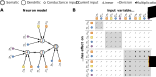
\includegraphics{media/chapter_multi_compartment_lif/nlif_product_terms.pdf}
	\caption[Effects of the relative location of input channels on the dendritic nonlinearity $H$]{Effects of the relative location of input channels on the dendritic nonlinearity $H$. \textbf{(A)}~Dendritic tree used in our example.
	The second compartment is only connected through the soma to the third and fourth compartment.
	\textbf{(B)} Table illustrating how pairs of input channels in \emph{(A)} interact according to \Cref{thm:nlif_product_terms}.
	Grey rectangles correspond to branches with nonlinear interaction.
	The symbol \enquote{$/$} indicates that $H$ only contains linear combinations of terms containing each variable; \enquote{$\div$} indicates that the variable in this column acts divisively on the other variable in the numerator; \enquote{$\bullet$} indicates that $H$ contains product terms with these two variables.}
	\label{fig:nlif_product_terms}
\end{figure}

\begin{theorem}
\label{thm:nlif_product_terms}
Consider an $n$-LIF neuron where each compartment is connected to $k$ unique con\-duc\-tance- and $k$ unique current-based input channels.
We denote these inputs as $g_j^i$ and $J_j^i$, where $i$ and $j$ are the compartment and input channel indices, respectively.
Furthermore, let all dendritic compartments with indices $i_{m - 1} + 1, \ldots, i_{m}$ (where $1 \leq m \leq \ell$) belong to the same connected component even if the somatic compartment is removed.
In this case, $H$ has the following form
\begin{align}
	H_0(g_1^1, \ldots, g_k^n, J_1^1, \ldots, J_k^1) +
	\frac{H^B_1(
		g_1^{2}, \ldots, g_k^{i_1} \!,
		J_1^{2}, \ldots, J_k^{i_1})
	}{
		H^A_1(g_1^{2}, \ldots, g_k^{i_1})
	}
	+ \ldots +
	\frac{H^B_\ell(
		g_1^{i_{\ell - 1} + 1}, \ldots, g_k^{i_\ell},
		J_1^{i_{\ell - 1} + 1}, \ldots, J_k^{i_\ell})
	}{
		H^A_\ell(g_1^{i_{\ell - 1} + 1}, \ldots, g_k^{i_\ell})
	} \,,
	\label{eqn:nlif_product_terms}
\end{align}
where (a) $H_0$ is an \emph{affine} function over all inputs injected into the somatic compartment, (b) the $H^A_i$ are nonnegative affine functions of product terms between conductanced-based inputs belonging to \emph{different} dendritic compartments that, and (c) the $H^B_i$ are affine functions of product terms between conductance-based input belonging to \emph{different} dendritic compartments, and \emph{at most one} dendritic current-based input per product term.
\end{theorem}

\subsubsection{Affine terms}
The \enquote{computationally weakest} $n$-LIF neurons are those where the somatic current is merely an affine function over the input channels.
As follows from \Cref{thm:nlif_product_terms}, this is the case for $n$-LIF neurons that only possess a somatic compartment, or, more generally, any $n$-LIF neuron where input is solely fed into the somatic compartment.
The same holds for $n$-LIF neurons that only possess current-based input channels.

\subsubsection{Shunting}
\Cref{thm:nlif_product_terms} similarly dictates that nonlinear interaction between the input channels of an individual dendritic compartment is limited to \enquote{shunting} \citep[cf.][Section~1.5]{koch1999biophysics}.
That is, conductance-based input channels act \enquote{divisively} on the other input channels in that compartment; they contribute to the denominator of one of the fractions in \cref{eqn:nlif_product_terms}.

Mathematically, this kind of nonlinear interaction is quite apparent in the dendritic nonlinearity for the two-compartment LIF neuron (eq.~\ref{eqn:two_comp_lif}); the excitatory and inhibitory conductances $g_\mathrm{E}$ and $g_\mathrm{I}$ act divisively on $H$.
The magnitude of this effect depends on the ratio between the input and the coupling- and leak-conductances.
Independent of the magnitude, and as we prove in \Cref{app:two_comp_xor_proof}, shunting in a single compartment cannot be used to compute \enquote{interesting} functions such as XOR:
\begin{theorem}
\label{thm:two_comp_xor}
Let $g_\mathrm{E}(x_1, x_2) = g_\mathrm{E}^1(x_1) + g_\mathrm{E}^2(x_2)$ and $g_\mathrm{I}(x_1, x_2) = g_\mathrm{I}^1(x_1) + g_\mathrm{E}^2(x_2)$ be nonnegative functions.
Furthermore, let $a_0 > 0$ and $a_1, a_2, b_0, b_1, b_2 \geq 0$.
Then, the two-compartment LIF nonlinearity
\begin{align*}
	\phi(x_1, x_2) = H(g_\mathrm{E}(x_1, x_2), g_\mathrm{I}(x_1, x_2)) &= \frac{b_0 + b_1 g_\mathrm{E}(x_1, x_2) - b_2 g_\mathrm{I}(x_1, x_2)}{a_0 + a_1 g_\mathrm{E}(x_1, x_2) + a_2 g_\mathrm{I}(x_1, x_2)}
\end{align*}
cannot be used to solve the weak XOR problem (see \Cref{def:weak_xor}).
\end{theorem}

Still, and as we demonstrate in the next section, a single layer of two-compartment LIF neurons can compute a wide range of functions with a substantially smaller error than a single layer, or, in some cases, even two layers of standard LIF neurons.

\subsubsection{Product terms}
Input channels targeting different dendritic compartments interact multiplicatively (cf. eq.~\ref{eqn:three_comp_lif_long}).
As we discussed above, multiplication over all four quadrants in $[-1, 1]^2$ can be interpreted as a continuous version of the XOR function.
However, exploiting the product terms in this manner is difficult for multiple reasons.
First, conductance-based inputs are nonnegative, and can thus only cover the quadrant $[0, 1]^2$.
While current-based channels can theoretically provide both positive and negative input, there is at most one current-based input per product term (cf.~\Cref{thm:nlif_product_terms}).

Second, the multiplicative terms are similar in magnitude to the linear terms---for example, all terms in the numerator in \cref{eqn:three_comp_lif_long} are the product of two conductances and one voltage, whereas all terms in the denominator at the product of two conductances.
This implies that, to compute a function such as XOR, we must find synaptic weights that compensate for the linear terms, while, at the same time, computing the desired nonlinear function.

Lastly, there is a tradeoff between the coupling conductances $c_{ij}$ and the maximum somatic current that can be produced by a compartment.
This current is proportional to the product of the intermediate coupling conductances, making it more difficult for distal compartments to influence the soma.
Countering this by choosing larger $c_{ij}$ results in more linear $H$.

Still, as we demonstrate in \Cref{sec:nlif_opt}, it is indeed possible to solve the weak XOR problem using a single three-compartment neuron.
In particular, we discuss an iterative weight optimisation scheme that quickly converges to locally optimal weights for any $n$-LIF neuron.

\section{Networks of Two-Compartment LIF Neurons}
\label{sec:two_comp_lif}

Up to this point, we have discussed the potential theoretical advantages of dendritic computation, extended the Neural Engineering Framework to support more complex connectivity constraints and neuron types, and introduced and analysed a family of multi-compartment LIF neurons with passive dendritic trees that we called \enquote{$n$-LIF} neurons.

The goal of this section is to systematically incorporate the simplest non-trivial $n$-LIF neuron---namely the two-compartment LIF neuron depicted in \Cref{fig:nlif_c}---into NEF networks.
This represents the smallest possible step toward exploiting dendritic nonlinearities, and as such is a good test for our overall methodology.

We proceed as follows.
First, we discuss a non-negative least-squares method for estimating the parameters of our surrogate dendritic nonlinearity model $H$.
We test the quality of the estimated parameters in various scenarios.
A similar approach can be used derive a quadratic program for the synaptic weights that takes nonnegative connectivity and subthreshold relaxation into account.
We use this approach to evaluate the theoretical advantage of the two-compartment LIF nonlinearity, akin to our experiment in \Cref{sec:dendritic_computation_theory_numerical}.
Finally, we demonstrate that this theoretical advantage persists in a spiking neural network context.

%TODO
%Interestingly, it is uncertain in how far shunting is actually exploited by biology.
%As reported in an empirical study by \citet{chance2002gain}, and in contrast to what has been suggested by previous theoretical work (e.g.,~\cite{koch1992multiplying}), it is implausible that individual input channels are responsible for implementing nonlinear functions such as nonnegative multiplication (\enquote{gain modulation}).
%For example, merely increasing $g_\mathrm{I}$ within biologically plausible bounds does not have a pronounced nonlinear effect.
%Instead, $g_\mathrm{E}$ and $g_\mathrm{I}$ must increase in tandem to evoke highly nonlinear responses.

%TODO: Three experiments

% TODO
%In practice, the maximum attainable current for realistic conductance values is significantly smaller than $J_\mathrm{max}$, limiting the maximum firing rate. This must be taken into account when selecting the neuron tuning curve.

\subsection{Estimating Model Parameters}
\label{sec:two_comp_lif_fit_model}

We presented the parametrised dendritic nonlinearity surrogate model $J = H(\gE, \gI)$ for two-compartment LIF neuron in \cref{eqn:two_comp_lif}.
While a coarse estimate of the model parameters $a_0$, $a_1$, $a_2$, $b_0$, $b_1$, $b_2$ can be derived from \cref{eqn:two_comp_lif_natural}, it is better to fit the parameters to empirical data.

To generate these data, we measure the current $J_k$ flowing into the somatic compartment for different input conductances $g_{\mathrm{E}, k}$, $g_{\mathrm{I}, k}$.
This can be accomplished by simulating the spiking neuron for a period of time $T$ and estimating the average spike rate $a_k = \mathscr{G}( g_{\mathrm{E}, k}, g_{\mathrm{I}, k})$.
As discussed in \Cref{sec:nef_nonlinear}, we obtain $J_k$ by applying the inverse of the chosen one-dimensional response curve $G^{-1}$ to $a_k$.
%From our experience, this method yields results superior to measuring $J_k$ directly in the simulation.
Importantly, when doing this, samples with small $a_k$ should be ignored: $G^{-1}$ is not well-defined for zero rates, and $H$ was derived for superthreshold dynamics.

\subsubsection{Optimisation problem}
Given the superthreshold samples $J_k$, $g_{\mathrm{E}, k}$, $g_{\mathrm{I}, k}$ we now have the following quadratic loss function over the parameters $a_i$, $b_i$:
\begin{align}
	E &=
		\sum_{k = 1}^N \bigl( J_k - H(g_\mathrm{E, k}, g_\mathrm{I, k}) \bigr)^2
	= \sum_{k = 1}^N \left( \! J_k - \frac{b_0 + b_1 g_{\mathrm{E}, k} - b_2 g_{\mathrm{E}, k}}{a_0 + a_1 g_{\mathrm{E}, k} + a_2  g_{\mathrm{I}, k}} \right)^2 \,,
	\;\; \begin{aligned}\text{subject to } a_0 &> 0 \,, \\ \text{and } a_1, a_2, b_0, b_1, b_2 &\geq  0 \,.\end{aligned}
	\label{eqn:two_comp_optimal_parameters}
\end{align}
Note that this optimisation problem has one superfluous degree of freedom.
A numerically stable normalisation is to set $b_1 = 1$.
In this case, all parameters are expressed relative to the effect of the excitatory channel on the input current.%
\footnote{As we mentioned in a footnote above, this is a result of the the scale-invariance of the individual rows of $\mat{\tilde A}$ and $\vec{\tilde b}$. In general, a parameterised $n$-LIF neuron has $n - 1$ superfluous degrees of freedom in its parameters.}

\begin{figure}
	\centering
	\includegraphics{media/chapter_multi_compartment_lif/two_comp_lif_loss_comparison.pdf}
	\caption[Comparison between the actual and substitute loss function.]{Comparison between the actual loss function (eq.~\ref{eqn:two_comp_optimal_parameters}; \textbf{A}) and the substitute loss function (eq.~\ref{eqn:two_comp_optimal_parameters_prime}; \textbf{B}).
	Each plot depicts a slice of the error function $E$ or $E'$ over two parameters.
	Black crosses correspond to the optimal solution with respect to the substitute loss function $E'$, black circles correspond to the closest local optimum in the actual loss function.
	The underlying data is sampled from a two-compartment LIF neuron with  $E_\mathrm{E} = \SI{20}{\milli\volt}$, $E_\mathrm{I} = \SI{-75}{\milli\volt}$, $E_\mathrm{L} = \SI{-65}{\milli\volt}$, $g_\mathrm{L} = \SI{50}{\nano\siemens}$, $c_{12} =\SI{30}{\nano\siemens}$ for $N = 318$ superthreshold samples of $\gE$, $\gI$ over $[\SI{0}{\nano\siemens}, \SI{500}{\nano\siemens}]$.
	The RMSE current error for the optimised weights is $\sqrt{E/N} = \SI{15.22}{\pico\ampere}$ when using the actual loss function for optimisation, and $\sqrt{E/N} = \SI{15.67}{\pico\ampere}$ when using the substitute loss function for optimisation ($3\%$ increase). The parameter $b_1$ is set to one.
	}
	\label{fig:two_comp_lif_loss_comparison}
\end{figure}

Unfortunately, \cref{eqn:two_comp_optimal_parameters} is neither in \emph{linear} least-squares form, nor convex.
%(see \Cref{app:two_comp_lif_non_convex}).
In theory, this complicates solving for model parameters \citep{rockafellar1993lagrange}.
Fortunately, we can largely work around this by minimising a convex substitute loss function (cf.~\Cref{fig:two_comp_lif_loss_comparison}).
Optimally, we like the following equality to hold for each sample $k$
\begin{align*}
	J_k &= H(g_{\mathrm{E}, k}, g_{\mathrm{I}, k}) = \frac{
		b_0 + b_1 g_{\mathrm{E}, k} - b_2 g_{\mathrm{I}, k}
	}{
		a_0 + a_1 g_{\mathrm{E}, k} + a_2 g_{\mathrm{I}, k}
 	} \Leftrightarrow 0 = J_k (a_0 + a_1 g_{\mathrm{E}, k} + a_2 g_{\mathrm{I}, k}) - b_0 - b_1 g_{\mathrm{E}, k} + b_2 g_{\mathrm{I}, k} \,.
\end{align*}
Notably, the two equations are equivalent because the denominator is strictly non-zero.
Phrasing this as a loss function for multiple samples yields
\begin{align}
	E' &= \sum_{k = 1}^N \bigl( J_k (a_0 + a_1 g_{\mathrm{E}, k} + a_2 g_{\mathrm{I}, k}) - b_0 - b_1 g_{\mathrm{E}, k} + b_2 g_{\mathrm{I}, k} \bigr)^2 \,,
	\label{eqn:two_comp_optimal_parameters_prime}
\end{align}
subject to the same constraints as above.
Arranging the samples in vectors $\vec J$, $\vec g_\mathrm{E}$, $\vec g_\mathrm{I} \in \mathbb{R}^N$, we can bring this into a canonical matrix form (where \enquote{$\circ$} is elementwise multiplication):
\begin{align}
	E' &= \|\mat A \vec \omega - \vec b \|_2^2 \,, & \text{where } \mat A = (\vec J, \vec J \, \circ \,  \vec g_\mathrm{E}, \vec J \, \circ \, \vec g_\mathrm{I}, -\vec{1}, \vec{g}_\mathrm{I}) \,, \; \vec b = \vec{g}_\mathrm{E} \,, \; \vec \omega &= (a_0, a_1, a_2, b_0, b_2) \,.
	\label{eqn:two_comp_optimal_parameters_prime_matrix}
\end{align}

Crucially, and as is illustrated in \Cref{fig:two_comp_lif_loss_comparison}, the solutions obtained by minimising \cref{eqn:two_comp_optimal_parameters,eqn:two_comp_optimal_parameters_prime} are similar, but not equivalent.
While both optimisation problems minimise the error for each sample, multiplication with the denominator in \cref{eqn:two_comp_optimal_parameters_prime} causes samples to be dynamically re-weighted.
Fortunately, at least in this application, the impact of this is fairly low in practice.
The global minimum of the substitute loss is typically close to a minimum in the actual loss function---though we technically cannot guarantee that this is a global minimum.

\subsubsection{Parameter refinement}
If an exact solution in terms of the closest local optimum of \cref{eqn:two_comp_optimal_parameters} is desired, the parameters can easily be refined using gradient descent.
Alternatively, and as originally suggested by \citet{sanathanan1963transfer} in the context of fitting transfer functions, we can refine the solution by iterative reweighting of \cref{eqn:two_comp_optimal_parameters_prime_matrix}.
Each sample is weighted by the inverse of its denominator from the previous iteration, i.e.,
\begin{align}
	E' &= \|\diag(\vec w)^{-1} \mat A \vec \omega - \diag(\vec w)^{-1}\vec b \|_2^2 \,, & \text{where } \vec w = a_0 \vec{1} + a_1 \vec g_\mathrm{E} + a_2 \vec g_\mathrm{I} \,.
	\label{eqn:sanathanan_koerner}
\end{align}
This scheme converges to a (not necessarily globally optimal) fixed point.
In our application this seems to be the case after two additional iterations.
A more thorough review of this \enquote{Sanathanan-Koerner iteration} is given in \citet[Section~2.2]{hokanson2018least}.
For the sake of simplicity, we chose not to rely on parameter refinement in our experiments.

\subsection{Experiment 1: Precision of the Model Parameter Estimation}
\label{sec:two_comp_lif_experiment_1}

The following experiment tests in how far the surrogate model $G[H(\gE, \gI)]$ can be used to accurately predict the spike rate $\mathscr{G}(\gE, \gI)$ of a simulated spiking two-com\-part\-ment LIF neuron---both before and after fitting the model parameters to empirical data.
We conduct this experiment in an artificial scenario with constant conductances \gE, \gI, and in a simulated network context with artificial temporal spike noise superimposed onto the inputs.

\begin{figure}[t]
	\includegraphics{media/chapter_multi_compartment_lif/model_parameter_fits_a.pdf}%
	{\phantomsubcaption\label{fig:synaptic_nonlinearity_fit_a_a}}%
	{\phantomsubcaption\label{fig:synaptic_nonlinearity_fit_a_b}}%
	\caption[Two-compartment dendritic nonlinearity model for constant input]{
		Two-compartment dendritic nonlinearity model for constant input. Contour plots depict measured average spike rates $\mathscr{G}(g_\mathrm{E}, g_\mathrm{I})$.
		Dashed lines are the model prediction $G[H(g_\mathrm{E}, g_\mathrm{I})]$. Dotted lines indicate the cross-section location.
		$E$ denotes the spike-rate RMSE over the regions where either the measured or predicted spike rate is greater than \SI{12.5}{\per\second}.
		Columns correspond to different coupling conductances $c_\mathrm{12}$.
		The model fits the numerical data well, with some deviations near the spike onset.}
	\label{fig:synaptic_nonlinearity_fit_a}%
\end{figure}

\subsubsection{Experiment 1.1: Constant conductances}
We analyse three two-compartment LIF neurons with coupling conductances $c_{12} = \SI{50}{\nano\siemens}$, $\SI{100}{\nano\siemens}$, and $\SI{200}{\nano\siemens}$; all other parameters are listed in \Cref{tbl:two_comp_neuron_parameters}.
We measure the output spike rate for constant input conductances $g_\mathrm{E}$, $g_\mathrm{I}$ on a $100 \times 100$ grid.
For each grid-point, the neuron's dynamical system (cf.~\Cref{sec:nlif_description}) is simulated for $T = \SI{1}{\second}$.
We then compute the steady-state firing rate by taking the inverse of the median inter-spike-interval.
The conductance range has been selected such that the maximum rate is \SI{100}{\per\second}, and the spike onset coincides with the diagonal of the \gE-\gI-rate contour plot.

We compare these numerical simulation results to both the theoretical somatic current prediction according to \cref{eqn:two_comp_lif_natural}, and the parameterised dendritic nonlinearity with the parameters fitted to the measured data.
Parameter optimization according to \cref{eqn:two_comp_optimal_parameters_prime_matrix} is based on a training-set of \num{200} conductance pairs sampled with uniform probability from the conductance-range.
The final prediction error is computed over all \num{10000} grid points.%
\footnote{As the next experiment produces a pronounced noise floor, we only consider rates above \SI{12.5}{\per\second} for fitting the model parameters and reporting the RMSE. For comparability, we use the same threshold in both experiments.}

\paragraph{Results}
The results for this experiment are depicted in \Cref{fig:synaptic_nonlinearity_fit_a}; the fitted parameters can be found in \Cref{tbl:two_comp_model_parameters}.
Unsurprisingly, when using the theoretical parameter estimate from \cref{eqn:two_comp_lif_natural}, there is a substantial discrepancy between the model prediction and the simulation, especially for large $c_{12}$ (\Cref{fig:synaptic_nonlinearity_fit_a_a}). This discrepancy is reduced after fitting the model parameters (\Cref{fig:synaptic_nonlinearity_fit_a_b}).
The model prediction fits the empirical data well for output spike rates greater than \SI{25}{\per\second}.
However, it fails to predict the spike onset correctly, placing it too early with respect to increasing \gE.
As we predicted in \Cref{sec:nlif_theory}, the linearity of $H$ increases as $c_{12}$ is increased, i.e., the contour lines become more \enquote{parallel} for larger $c_{12}$.

\paragraph{Discussion}
Overall, the model works well once the parameters have been fitted.
The mismatch between measured rates and the theoretical model for large $c_{12}$ is likely due to the more pronounced effect of the somatic superthreshold dynamics on the dendritic compartment.
Failure to predict the spike onset is likely due to our model not capturing low firing-rate regimes of the neuron well.

\subsubsection{Experiment 1.2: Conductances with artificial temporal spike noise}

\begin{figure}[t]
	\includegraphics{media/chapter_multi_compartment_lif/model_parameter_fits_b.pdf}%
	\caption[Two-compartment dendritic nonlinearity model for noisy input]{Two-compartment dendritic nonlinearity model for noisy input with combined excitatory Poisson spike rates of $1/\lambda = \SI{4500}{\per\second}$ for excitatory synapses and $1/\lambda = \SI{1800}{\per\second}$ for inhibitory synapses.
	See \Cref{fig:synaptic_nonlinearity_fit_a} for a complete legend.
	The model fits the noisy data better than the noise-free data.
	    }
	\label{fig:synaptic_nonlinearity_fit_b}%
\end{figure}

In a network context, \gE and \gI are not constant, but, as we discussed in Section~2.2.2, a weighted sum of low-pass filtered spike trains.
This results in a considerable amount of \enquote{spike noise} in the conductance inputs.
In this experiment, we generate artificial filtered spike trains using spike times from Poisson sources (simulation period $T = \SI{100}{\second}$; rates fitted to data from Experiment~3; see below).
Synaptic weights are simulated by uniformly sampling scaling factors for each spike event.
The resulting signals are scaled such that the averages conductances are equal to \gE, \gI.
We de
We furthermore replace $G[J]$ with a ReLU, that is $G[J] = \max\{ 0, \alpha J + \beta \}$.
We know from preliminary experiments that the hard LIF spike-onset is not present in noisy environments---this is not captured well by the standard LIF response curve.
While we could use a \enquote{soft} version of the LIF response curve that takes this into account \citep[cf.][]{capocelli1971diffusion,hunsberger2014competing,kreutz2015mean}, a ReLU appears to work well.

\paragraph{Results}
The results of this experiment are depicted in \Cref{fig:synaptic_nonlinearity_fit_b}.
Final fitted parameters are provided in \Cref{tbl:two_comp_model_parameters}.
Surprisingly, our model fits the noisy spike rates better than non-noisy data.
Still, the overall trends from the previous experiment are still visible.
When using the theoretical parameter estimates, larger $c_{12}$ result in higher overall errors and fitting the model parameters greatly reduces the error to values below \SI{1}{\per\second} for spike rates greater than \SI{12.5}{\per\second}.
While the sharp spike onset is no longer present, the model does not capture the subtle sigmoid shape of the response curve near the spike onset that is particularly pronounced for larger $g_\mathrm{C}$.

\paragraph{Discussion}
To summarize, our results indicate that, after fitting the model parameters, the surrogate model $H$ can indeed be used to predict the neural response curve $\mathscr{G}(\gE, \gI)$ with a relatively high accuracy in both tested scenarios.
It seems reasonable to choose a different one-dimensional neural response curve $G[J]$ when taking noise in the input into account.


\subsection{Solving for Synaptic Weights}

We demonstrated that the surrogate model $H(\gE, \gI)$ can be used to quite accurately predict the firing rates of individual two-compartment LIF neurons.
Now, to construct NEF networks, we must find weights $\vec w^\mathrm{E}_i$, $\vec w^\mathrm{I}_i$ that fulfil the normative tuning-curve constraint from \cref{eqn:dendritic}.

\subsubsection{Optimisation problem}
Given a function $f(\vec x)$ that we would like to compute, we optimally minimise the following least-squares loss over $\vec w^\mathrm{E}_i$, $\vec w^\mathrm{I}_i$ for each post-neuron $i$
\begin{align}
	E &= \frac{1}{\Xrepr} \int_{\Xrepr} \mathcal{E} \left( J_i(f(\vec x)), \frac{
		b_0 + b_1 \langle \vec w^\mathrm{E}_i, \vec a(\vec x) \rangle - b_2 \langle \vec w^\mathrm{I}_i, \vec a(\vec x) \rangle
	}{
		a_0 + a_1 \langle \vec w^\mathrm{E}_i, \vec a(\vec x) \rangle + a_2 \langle \vec w^\mathrm{I}_i, \vec a(\vec x) \rangle
 	}	
	\right)^2 \, d\vec x + \sigma^2 \| \vec w^\mathrm{E}_i \|^2_2 + \sigma^2 \| \vec w^\mathrm{I}_i \|^2_2 \,,
	\label{eqn:two_comp_optimal_weights}
\end{align}
subject to $\vec w^\mathrm{E}_i$, $\vec w^\mathrm{I}_i \geq 0$,
and where $\mathcal{E}$ is the superthreshold error function (eq.~\ref{eqn:subthreshold_error}), $\vec a(\vec x)$ are the stacked pre-activities of all pre-populations, and $J_i(\vec x)$ is the current-translation function.

Just like the model parameter optimisation problem from the previous subsection, \cref{eqn:two_comp_optimal_weights} is not convex.
%(again, see \Cref{app:two_comp_lif_non_convex} for more details).
Again, we work around this by multiplying with the denominator inside the square to obtain a substitute loss function:
\begin{align}
	\begin{aligned}
	E' &=
		\int_{\Xrepr} \mathcal{E}
		\Bigl(
			J_i(f(\vec x)) (a_0 + a_1 \langle \vec w^\mathrm{E}_i, \vec a(\vec x) \rangle + a_2 \langle \vec w^\mathrm{I}_i, \vec a(\vec x) \rangle )\,, \\[-1em]
		&\hspace{3.66em}		
		b_0 + b_1 \langle \vec w^\mathrm{E}_i, \vec a(\vec x) \rangle - b_2 \langle \vec w^\mathrm{I}_i, \vec a(\vec x) \rangle
		\Bigr)^2 \, d\vec x
		 + \sigma^2 \| \vec w^\mathrm{E}_i \|^2_2 + \sigma^2 \| \vec w^\mathrm{I}_i \|^2_2 \,,
	\end{aligned}
	\label{eqn:two_comp_optimal_weights_prime}
\end{align}
subject to $\vec w^\mathrm{E}_i$, $\vec w^\mathrm{I}_i \geq 0$.
A sampled version of this problem can be phrased as a quadratic program.
To see this, let $\mat A \in \mathbb{R}^{N \times n}$ be a matrix of pre-activities and $\vec J_i \in \mathbb{R}^{N}$ be a vector of target currents.
Assume that we only have superthreshold samples, that is $\mathcal{E}(J_\mathrm{tar}, J_\mathrm{dec}) = J_\mathrm{tar} - J_\mathrm{dec}$. We have:
\begin{align}
	E' &\propto \bigl\|	\,
		  \vec J_i \circ
		  	\bigl(
		  		a_0 +
		  		a_1 \mat{A} \vec w_i^\mathrm{E} +
		  		a_2 \mat{A} \vec w_i^\mathrm{E} \bigr)
	      - \bigl(
	      		b_0 +
	      		b_1 \mat{A} \vec w_i^\mathrm{E} -
	      		b_2 \mat{A} \vec w_i^\mathrm{I} \bigr)
	\, \bigr\|_2^2
	+ \sigma^2 \bigl\| \vec w^\mathrm{E}_i \bigr\|^2_2 + \sigma^2 \bigl\| \vec w^\mathrm{I}_i \bigr\|^2_2 \notag \\
		&= \hspace{0.125em} \bigl\|
			\bigl(a_1 \diag(\vec J_i) \mat A - b_1 \mat A \bigr) \vec w_i^\mathrm{E}
			+ \bigl(a_2 \diag(\vec J_i) \mat A + b_2 \mat A \bigr) \vec w_i^\mathrm{I}
			+ (a_0 - b_0) \vec J_i
	\, \bigr\|_2^2
	+ \sigma^2 \bigl\| \vec w^\mathrm{E}_i \bigr\|^2_2 
	+ \sigma^2 \bigl\| \vec w^\mathrm{I}_i \bigr\|^2_2  \notag \\
	&= \hspace{0.125em} \bigl\|
		\mat A' \vec w_i + \vec J_i'
	\bigr\|_2^2
	+ \sigma^2 \bigl\| \vec w_i \bigr\|^2_2  \,.
	\label{eqn:two_comp_optimal_weights_prime_matrix}
\end{align}
To account for subthreshold relaxation, we simply split $\mat A'$ and $\vec J'$ into super- and subthreshold samples as discussed in \Cref{sec:nef_subthreshold} and use the QP defined in \cref{eqn:decode_subthreshold_qp}.

Of course, we could use the Sanathanan-Koerner iteration (cf.~eq.~\ref{eqn:sanathanan_koerner}) to refine the solution.
However, in our experience, and as with the parameter optimisation problem, the solution to the convex problem tends to be close to a local optimum in the original rational loss function.

\subsubsection{Example: Addition and gain modulation}
Although we analyse two-compartment neurons more thoroughly in the next two sections, we would first like to test our weight optimisation scheme in the context of two specific functions $f$: addition and nonnegative multiplication.

Specifically, we use the two-compartment LIF neuron with $c_{12} = \SI{50}{\nano\siemens}$ (parameter set (ii) from \Cref{tbl:two_comp_neuron_parameters})
%As we will see, two-compartment LIF neurons can compute addition just as well as standard LIF neurons, while being substantially better at nonnegative multiplication.
and the network setup discussed in
\Cref{sec:dendritic_computation_theory_dendritic}.
That is, two pre-populations with 200 neurons each project onto a single post-neuron; the pre-populations represent $x_1$, $x_2$, respectively, while the post-neuron represents $\hat y \approx f(x_1, x_2)$.%
\footnote{While an individual neuron is not sufficient for reconstructing the represented value $\hat y$ via linear decoding, we can infer $\hat y$ by inverting the current translation function; that is $\hat y = J^{-1}[H(\gE(x_1) + \gE(x_2), \gI(x_1) + \gI(x_2))]$.
Our post-neuron has a positive encoder, an $x$-intercept of zero, and a maximum rate of \SI{100}{\per\second}.
}
As depicted in \Cref{fig:nef_multivariate_functions_c}, the synaptic weights implicitly define a set of conductance functions.
Due to commutativity of addition and multiplication, the excitatory and inhibitory functions decoded from each pre-population optimally are the same; we have $\gE(x) = g_\mathrm{E}^1(x) = g_\mathrm{E}^2(x)$ and $\gI(x) = g_\mathrm{I}^1(x) = g_\mathrm{I}^2(x)$.
We emulate current-based LIF neurons by setting $a_0 = b_1 = 1$, $b_2 = -1$, and $a_1 = a_2 = b_0 = 0$ in the nonlinearity model $H$.
For these parameters we have $H(J_\mathrm{E}, J_\mathrm{I}) = J_\mathrm{E} - J_\mathrm{I}$.
%while the synaptic weights implicitly describe excitatory and inhibitory current functions $J_\mathrm{E}(x)$ and $J_\mathrm{I}(x)$.

\begin{figure}
	\centering
	\includegraphics{media/chapter_multi_compartment_lif/two_comp_weights_examples_addition.pdf}%
	{\phantomsubcaption\label{fig:two_comp_weights_examples_addition_a}}%
	{\phantomsubcaption\label{fig:two_comp_weights_examples_addition_b}}%
	\caption[Computing addition in single- and two-compartment LIF neurons]{Computing addition in \textbf{(A)} single- and \textbf{(B)} two-compartment LIF neurons. See text for a detailed description. \emph{Top:} Decoded current and conductance functions. \emph{Left:} Decoded represented value. Black contour lines and coloured backdrop correspond to the decoded values $\hat y$; dashed white lines to the target function $y$. \emph{Right:} Decoding error $\hat y - y$. Depicted error value $E$ is the NRMSE.
	Single- and two-compartment LIF neurons are equally suitable for computing linear functions.
	}
	\label{fig:two_comp_weights_examples_addition}
\end{figure}

%\paragraph{Results: Addition}
Results for computing addition, that is $f(x_1, x_2) = \frac{1}2 (x_1 + x_2)$ over $(x_1, x_2) \in [0, 1]^2$, are depicted in \Cref{fig:two_comp_weights_examples_addition}.
As is expected, we can compute this function with a low NRMSE with the current-based nonlinearity.
Perhaps unintuitively, and in spite of the dendritic nonlinearity $H$, we achieve similarly low errors using the two-compartment LIF neuron.

The way in which the weight solver accomplishes this becomes apparent when considering the decoded current functions \gE and \gI in \Cref{fig:two_comp_weights_examples_addition_b}.
Both $\gE$ and $\gI$ are affine functions with opposing slopes.
Correspondingly, the denominator $a_0 + a_1 \gE + a_2 \gI$ stays approximately constant, while the numerator $b_0 + b_1 \gE - b_2 \gI$ generates the desired target currents.


\begin{figure}
	\centering
	\includegraphics{media/chapter_multi_compartment_lif/two_comp_weights_examples_multiplication.pdf}%
	{\phantomsubcaption\label{fig:two_comp_weights_examples_multiplication_a}}%
	{\phantomsubcaption\label{fig:two_comp_weights_examples_multiplication_b}}%
	\caption[Computing multiplication in single- and two-compartment LIF neurons]{Computing multiplication in \textbf{(A)} single- and \textbf{(B)} two-compartment LIF neurons. See text for a detailed description and \Cref{fig:two_comp_weights_examples_addition} for a legend. Nonnegative multiplication can be reasonably well approximated using two-compartment LIF neurons. Dotted line in \emph{(B)} is a hyperbolic fit.
	}
	\label{fig:two_comp_weights_examples_multiplication}
\end{figure}

%\paragraph{Results: Multiplication}
Results for computing nonnegative multiplication, that is $f(x_1, x_2) = x_1 x_2$ over $(x_1, x_2) \in [0, 1]^2$, are depicted in \Cref{fig:two_comp_weights_examples_multiplication}.
Using current-based LIF neurons we can, at best, approximate multiplication with a linear function. This results in an NRMSE of about 25\%.
In contrast, using the two-compartment LIF nonlinearity results in an error of about 6\%, with the largest discrepancies being in regions are both $x_1$ and $x_2$ are close to one.


\begin{figure}
	\centering
	\includegraphics{media/chapter_multi_compartment_lif/two_comp_weights_examples_statistics.pdf}%
	{\phantomsubcaption\label{fig:two_comp_weights_examples_statistics_a}}%
	{\phantomsubcaption\label{fig:two_comp_weights_examples_statistics_b}}%
	{\phantomsubcaption\label{fig:two_comp_weights_examples_statistics_c}}%
	{\phantomsubcaption\label{fig:two_comp_weights_examples_statistics_d}}%
	\caption[Error and weight statistics for computing addition and nonnegative multiplication]{Error and weight statistics for computing addition and nonnegative multiplication. \textbf{(A, B)}
	
	Depicted is the median over $1000$ experiments, shaded areas the 25/75-percentiles.
	While errors monotonically decreases with more pre-neurons in the addition task \emph{(A)}, errors quickly plateau when computing multiplication \emph{(B)}.
	\textbf{(C,~D)}~Comparison between the weight magnitude frequencies for the two tasks and neuron types (for $n = 300$ pre-neurons).
	Weights are normalised such that a value of one corresponds to $\SI{1}{\nano\ampere}$ or $\SI{1}{\nano\siemens}$, respectively.
	Dashed line and depicted values are the median; frequencies include zero-weights. Weights below $10^{-6}$ are counted as zero. Two-compartment LIF neurons require larger weight magnitudes. The spread of the magnitudes changes depending on the computed function.
	}
	\label{fig:two_comp_weights_examples_statistics}
\end{figure}

Importantly, and as is depicted in \Cref{fig:two_comp_weights_examples_statistics_b}, two-compartment LIF neurons cannot approximate nonnegative multiplication with an arbitrarily small error; more precisely, the error cannot be reduced past 6\% for a single post-neuron.
This is in contrast to addition, where we can reach arbitrarily small errors by increasing the number of pre-neurons (cf.~\Cref{fig:two_comp_weights_examples_statistics_a})
It is possible to reach smaller (but not arbitrarily small) errors with multiple post neurons dividing up the represented space (we reach down to $4\%$; see $E_\mathrm{model}$ in \Cref{tbl:function_approximations_complete}).

Curiously, looking at the conductance functions \gE and \gI, \emph{both} excitation and inhibition increase substantially for small $x_1$ or $x_2$, similar to a shifted and scaled hyperbola  $(\beta + \alpha x)^{-1}$ (black dotted line in \Cref{fig:two_comp_weights_examples_multiplication_b}).
This may be counter-intuitive, given that inhibition is typically responsible for shutting off the target neuron.%
\footnote{Remember that these results are for a single post-neuron with positive encoder. That is, to represent smaller values, the neuron must receive a smaller input current.}
However, when increasing both excitation and inhibition, this common-mode increase mostly cancels out in the numerator (due to the inhibitory conductance being subtracted), but increases the magnitude of the denominator; this amplifies the divisive effect of the input.

Notably, nonnegative multiplication (or, alternatively, nonnegative division) is also referred to as \enquote{gain modulation} in the neuroscience literature.
The observation that both excitation and inhibition must be increased to multiplicatively (or divisively) reduce the gain of a neuron is consistent with \emph{in vitro} experiments \citep{chance2002gain}.

An earlier hypothesised mechanism for gain modulation is \emph{shunting inhibition}.
Here, the idea is that an inhibitory channel with a reversal potential close to the resting potential acts divisively on the average input current.
This effect could in theory be used to implement multiplication \citep{koch1992multiplying}; however, in practice, increasing inhibitory conductances alone has a predominantly linear effect on the spike rate (since $a_2 \ll b_2$), or requires implausibly high conductance values \citep{holt1997shunting,abbott2005drivers}.

Even when exploiting the common increase of excitation and inhibition, generating the large input conductances for small $x_1$, $x_2$ results in relative large synaptic weights.
This is depicted in \Cref{fig:two_comp_weights_examples_statistics_c,fig:two_comp_weights_examples_statistics_d}.
Compared to computing addition, the median synaptic weight increases by a factor of five.

\subsection{Experiment 2: Theoretical Analysis of Two-Compartment LIF Neurons}
\label{sec:two_comp_lif_experiment_2}

The goal of this and the next subsection is to analyse the two-compartment nonlinearity in a more systematic manner.
First, our goal is to analyse the theoretical advantage of the two-comaprtment LIF nonlinearity $H$ compared to current-based neurons, similar to our experiment in \Cref{sec:dendritic_computation_theory_numerical}.
We do this under the implicit assumption that $H$ accurately describes the somatic current---as is suggested by our earlier results from Experiment~1 (\Cref{sec:two_comp_lif_experiment_1}).

\subsubsection{Methods}
Just as in \Cref{sec:dendritic_computation_theory_numerical}, we would like to measure how well a system can approximate functions of increasing complexity.
To this end, we use the bandwith of randomly generated 2D-functions as a proxy for \enquote{complexity}; the bandwidth is inversely proportional to the low-pass filter coefficient $\sigma$ (cf.~\Cref{fig:2d_functions_overview}).
The generated current functions $J_\sigma(x_1, x_2)$ are sampled over $(x_1, x_2) \in [-1, 1]^2$ on a $63 \times 63$ grid, and normalized such that the mean is zero and the standard deviation equals $\SI{1}{\nano\ampere}$.
We measure how well we can approximate this desired post synaptic current for a single post-neuron with a given input-dependent nonlinearity.

Again, we use the network setup depicted in \cref{fig:nef_multivariate_functions_c}.
Two pre-populations with \num{100} neurons each represent $x_1$ and $x_2$, respectively.
All neurons project both excitatorily and inhibitorily onto a single post-neuron.
The population tuning curves are randomly generated in each trial with a maximum firing rate between \num{50} and \SI{100}{\per\second} per neuron.

All synaptic weights are computed by solving the QP in \cref{eqn:two_comp_optimal_weights_prime_matrix} for 256 randomly selected training samples, both with and without subthreshold relaxation.
The regularisation parameters were selected independently for each setup, as is depicted in \Cref{fig:2d_regularisation_sweep}.
The final error is the NRMSE (relative to the standard deviation of $\SI{1}{\nano\ampere}$ of $f_\sigma$) over all \num{3969} grid points.
We add normal distributed noise (zero mean, unit standard deviation) to the pre-activities when computing the error to test how well the computed weights generalise.

We compare the conductance-based two-compartment LIF nonlinearity (abbreviated as $H_\mathrm{cond}$) to the current-based $H_\mathrm{cur}(J_\mathrm{E}, J_\mathrm{I}) = J_\mathrm{E} - J_\mathrm{I}$.
As a further point of comparison, we include a \enquote{two-layer} neural network setup (\cref{fig:nef_multivariate_functions_b}). The 200 pre-neurons are tuned to both input dimensions $(x, y)$, and not $x$ and $y$ independently.

\begin{figure}[p]
	\centering
	\raisebox{135.86mm}{\includegraphics{media/chapter_multi_compartment_lif/two_comp_2d_frequency_sweep.pdf}}%
	\kern-158.06mm\includegraphics{media/chapter_multi_compartment_lif/two_comp_2d_frequency_sweep_overlay.pdf}
	\begin{subfigure}{0cm}\phantomcaption\label{fig:frequency_sweep_a}\end{subfigure}%
	\begin{subfigure}{0cm}\phantomcaption\label{fig:frequency_sweep_b}\end{subfigure}%
	\caption[Decoding error for random multivariate current functions]{Decoding error for random multivariate current functions. Continued on next page.}
	\label{fig:two_comp_lif_frequency_sweep}
\end{figure}

\addtocounter{figure}{-1}
\begin{figure}[t]
	\caption[]{Decoding error for random multivariate current functions.
	\textbf{(A)} NRMSE between random, two-dimensional current functions and the decoded approximation using different input-dependent nonlinearities. The error measurement does not take subthreshold currents into account, using the function $\mathcal{E}$ defined in \cref{eqn:decode_current_subthreshold}. The low-pass filter coefficient $\sigma^{-1}$ is a proxy for the spatial frequency content in the target function. All points correspond to the median over \num{1000} trials. Dashed lines show results for not taking the subthreshold relaxation into account when solving for weights. The black lines show the results for a linear, current-based $H_\mathrm{cur}$; blue/green lines show the results for the two-compartment conductance-based model  $H_\mathrm{cond}$ with parameters given in \Cref{tbl:model_parameters} (without noise). Orange lines correspond a current-based network with two-dimensional pre-neuron tuning (i.e., a two-layer neural network). Shaded areas correspond to the 25/75 percentile for the current-based models and the conductance-based model with $c_{12} = \SI{50}{\nano\siemens}$.
	\textbf{(B)} Exemplary random functions and the corresponding decodings. Deep violet regions (dashed contour lines) correspond to subthreshold currents. Note how the shape of the subthreshold contour lines no longer match the target when subthreshold relaxation is active. As visible, the conductance-based nonlinearity $H_\mathrm{cond}$ helps to decode some target functions with a drastically smaller error compared to the current-based model $H_\mathrm{cur}$, especially when comparing the setups without subthreshold relaxation. $H_\mathrm{cond}$ does not provide any benefit for target functions with a high bandwidth.
	}
	\rule{\columnwidth}{1pt}
\end{figure}

\subsubsection{Results}
Results are depicted in \Cref{fig:two_comp_lif_frequency_sweep}. For a current-based neuron, and without subthreshold relaxation (dashed line in the plot), the median error increases linearly on a log-log plot from a $2.5\%$ error for low-frequency---almost linear---functions to an error of about $50\%$ for functions with a spatial cut-off frequency greater than one. Subthreshold relaxation reduces this error by up to $50\%$ for low $\sigma^{-1}$.

The error for the conductance-based nonlinearity increases sub-linearly on a log-log plot, starting at median errors of about $0.8\%$ for low-frequency functions. It is competitive with the two-layer network (see below) for $\sigma^{-1} < 0.5$. The error function converges to the results for the current-based model for spatial frequencies $\sigma^{-1} > 1$. Overall, the error for the conductance-based model is reduced by up to $65\%$ compared to the current-based model. The benefits of subthreshold relaxation are not as pronounced as for the linear current model.

The large errors for the current-based and the conductance-based models for $\sigma^{-1} > 1$ can be explained by the fact that both functions cannot be used to solve the XOR problem (cf.~\Cref{app:xor}). Functions with $\sigma^{-1} \geq 1$ are likely to possess multiple maxima/minima over $[-1, 1]^2$, akin to XOR, leading to a large error.

The two-layer network setup is able to approximate functions well up to $\sigma^{-1} = 10$, where it reaches the same final error values as the other setups. The complexity of the functions that can be approximated well by this setup is limited by the number of pre-neurons. The two-layer network can be thought of as linearly combining rectified hyperplanes to fit the target function, where each hyperplane is a single pre-neuron response. At a certain $\sigma$, the number of hyperplanes is no longer sufficient to reconstruct all the local maxima/minima in the target function.

\subsubsection{Discussion}
To summarise, this experiment demonstrates that the two-compartment LIF dendritic nonlinearity $H$ significantly reduces the approximation error of current functions with $\sigma^{-1} < 1$ in a network setup with pre-populations independently representing the input dimensions. It is competitive with a two-layer network for $\sigma^{-1} < 0.5$.


\subsection{Experiment 3: Dendritic computation of multivariate functions in spiking network models}
\label{sec:dendritic_computation_network}
Unless explicitly specified, the neuron model parameters are chosen according to \Cref{tbl:parameters}.  We model fast excitatory synapses as an exponential low-pass with a time-constant of \SI{5}{\milli\second} as found in glutamatergic pyramidal neurons with AMPA receptor \citep{jonas1993quantal}. The inhibitory pathway is modeled with a \SI{10}{\milli\second} time-constant as found in inhibitory interneurons with GABA\textsubscript{A} receptors \citep{gupta2000organizing}.

Experiment 1 suggests that we can use the non-linear post-synaptic current model $H$ to predict the average current flowing into the somatic compartment. Experiment 2 shows that we can, assuming that $H$ accurately describes the somatic current, approximate a somewhat larger class of random functions well. In our final experiment we study whether we can still observe the reduction in error in a feed-forward spiking neural network when using our model $H$ to solve for weights.

In contrast to previous experiment we do not base our error measurements on the decoded static somatic current for a \emph{single} post-neuron. Instead we decode the represented value from the neural activities of a target \emph{population} over time. Optimally, this decoded value should be $f(x(t), y(t))$, where $f$ is the function that we want to approximate and $x(t), y(t) \in [-1, 1]$ are input signals in turn represented by populations of \num{100} LIF neurons each. The target population either consists of standard current-based LIF neurons (\cref{fig:network_a}) or conductance-based two-compartment neurons (\cref{fig:network_c}).

Just as in the previous experiment, we consider the two-layer topology in \cref{fig:network_b} as a point of reference. Here, the input is mediated via an additional layer of \num{200} neurons representing the vectorial quantity $(x(t), y(t))$ over the interval $[-1, 1]^2$.

For all neurons, we generate tuning curves such that the maximum firing rate falls between \num{50} and \SI{100}{\per\second} over their represented range. Neurons are randomly marked as either excitatory or inhibitory. The probability of a neuron being inhibitory is 30\%. Excitatory and inhibitory synapses are modeled as a first-order exponential low-pass filter with time-constants of $\tau_\mathrm{E} = \SI{5}{\milli\second}$ and $\tau_\mathrm{I} = \SI{10}{\milli\second}$, respectively.

The network is simulated over \SI{10}{\second} at a time-resolution of \SI{100}{\micro\second}. Inputs $x(t)$ and $y(t)$ are sampled by moving through time along a fourth-order space-filling Hilbert curve over $[-1, 1]^2$. The output of the target population is decoded and filtered with a first-order exponential low-pass at $\tau = \SI{100}{\milli\second}$. We compute the desired target value $f(x, y)$ from the original input and pass it through the same series of low-pass filters as the spiking signals. We use the average synaptic time-constant of \SI{7.5}{\milli\second} to emulate the effect of the synaptic low-pass filters. Our final measure $E_\mathrm{net}$ is the normalized RMSE between the decoded output and the target values over time; the normalization is relative to the standard deviation of the target signal.

All synaptic weights are computed by solving the QP in \cref{eqn:conductance_qp}, with the same mapping of the current-based onto the conductance-based model as in Experiment 2. The regularization term $\lambda$ has been chosen independently for each neuron type and model parameter set such that the network error $E_\mathrm{net}$ is minimized when computing multiplication (cf.~\cref{fig:regularization_parameter_sweep}).

\subsubsection*{Experiment 3.1: Random bandlimited functions}

\begin{figure}[t]
	\centering
	{\includegraphics{media/chapter_multi_compartment_lif/two_comp_2d_frequency_sweep_network.pdf}}%
	\kern-158.06mm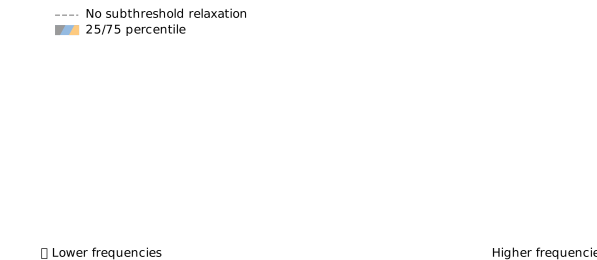
\includegraphics{media/chapter_multi_compartment_lif/two_comp_2d_frequency_sweep_network_overlay.pdf}
	\caption[Median error for computing random bandlimited functions in a feed-forward network over 1000 trials.]{Median error for computing random bandlimited functions in a feed-forward network over 1000 trials. Measured NRMSE is the difference between the represented value $\hat y(t)$ and the expected value $f_\sigma(x_1(t), x_2(t))$ relative to the standard deviation of $f_\sigma$. See \Cref{fig:frequency_sweep_a} for more detail.}
	\label{fig:frequency_sweep_network}
\end{figure}

We first test our network setup with the random bandlimited functions $f_\sigma$ we already used in the previous experiment. Results are depicted in \cref{fig:frequency_sweep_network}. Qualitatively, the results are very similar to what we saw before. The reduction in error between the current- and conductance-based models is not quite as large as suggested by the theoretical experiment, with a maximum reduction (in terms of the median) of only $45\%$ (instead of $65\%$ before). While subthreshold relaxation mostly increased the performance of the current-based model in the previous experiment, the improvement in error is now clearly visible for the conductance-based model as well.

Notably, the minimum median approximation error of the two-layer network is about $10\%$, whereas the single-layer current- and conductance-based models reach minimum errors of about $6.5\%$ and $5\%$, respectively. The two-layer network clearly surpasses the performance of the two-compartment LIF single-layer network for $\sigma^{-1} > 0.6$.
The larger errors are mainly caused by the representation of the two-dimensional quantity $(x(t), y(t))$ begin noisier than the representation of the scalars $x(t)$, $y(t)$ in the two pre-populations. This is because chaining multiple populations of spiking neurons slightly increases the noise floor. Furthermore, to cover the square $[-1, 1]^2$ as densely as two one-dimensional intervals $[-1, 1]$, we would optimally have to square the number of neurons. In our case, we would have to use \num{10000} instead of \num{200} neurons for the intermediate layer, which would not really be comparable to the single-layer setups---keep in mind that the two-layer network already uses $66\%$ more neurons.



\subsubsection*{Experiment 3.2: Benchmark functions}

\begin{figure}
	\includegraphics{media/chapter_multi_compartment_lif/two_comp_network_spikes_example.pdf}
	\caption[Single spiking neuron experiment showing computation of multiplication using a two-compartment LIF neuron.]{Single spiking neuron experiment showing computation of multiplication using a two-compartment LIF neuron.
	\textbf{(A)} \emph{Top two plots:} inputs $x_1(t)$ and $x_2(t)$ as represented by the two pre-populations. The input is a fourth order 2D Hilbert curve. \emph{Bottom:} mathematical target $f(x_1(t), x_2(t)) = x_1(t) x_2(t)$, filtered target function, as well as the decoded target population output.
	\textbf{(B)} Spike raster plots corresponding to the spiking activity of each of the populations (only half of the neurons are depicted). Red shaded background corresponds to inhibitory neurons in the pre-populations, all other neurons are excitatory.}
	\label{fig:spiking_example}
\end{figure}

\begin{table}[t]
	\caption[Spiking neural network approximation errors.]{Spiking neural network approximation errors for function approximations on $[0, 1]^2$. Error values correspond to the NRMSE and are measured as the difference between the output decoded from the target population and the desired output for a ten second sweep across a 4th order 2D Hilbert curve over the input space. Results are the mean and standard deviation over 256 trials. The best result for a target function is set in bold; darker background colours indicate a worse ranking of the result in the corresponding row. Columns labeled \enquote{standard} refer to the default, single layer network setup, \enquote{two layers} refers to the two-layer setup, and \enquote{noise model} to the single layer network setup with model parameters derived under noise (see Experiment 1.2). Additional tables can be found in \Cref{app:two_comp_lif_results}.}
	%--------------------------------------------
	\fontsize{9.5pt}{12pt}\selectfont
	\sffamily
	\renewcommand\arraystretch{1.5}
	\centering
	\begin{tabular}{r r r r r r r r }
	\toprule
	\textbf{Target}& \multicolumn{7}{c}{\textbf{Experiment setup}} \\
	\cmidrule(r){1-1}\cmidrule(l){2-8}
	& \multicolumn{3}{c}{%0
	LIF}
	& \multicolumn{2}{c}{%1
	Two comp. LIF $c_{12} = \SI{50}{\nano\siemens}$}
	& \multicolumn{2}{c}{%2
	Two comp. LIF $c_{12} = \SI{100}{\nano\siemens}$}
	\\
	\cmidrule(l){2-4}
	\cmidrule(l){5-6}
	\cmidrule(l){7-8}
	& standard
	& standard\textsuperscript{\dag}
	& two layers\textsuperscript{\dag}
	& %0
	standard\textsuperscript{\dag}
	& %1
	noise model\textsuperscript{\dag}
	& %0
	standard\textsuperscript{\dag}
	& %1
	noise model\textsuperscript{\dag}
	\\
	\midrule
	$x + y$ 
	& \cellcolor{White!72!SteelBlue}$4.2 \pm 0.3\%$
	& \cellcolor{White!58!SteelBlue}$4.2 \pm 0.3\%$
	& \cellcolor{White!29!SteelBlue}$8.2 \pm 0.4\%$
	& \cellcolor{White!100!SteelBlue}$\mathbf{2.3 \pm 0.3\%}$
	& \cellcolor{White!43!SteelBlue}$7.1 \pm 0.8\%$
	& \cellcolor{White!86!SteelBlue}$3.7 \pm 0.4\%$
	& \cellcolor{White!15!SteelBlue}$8.3 \pm 0.9\%$
	\\
	$x \times y$ 
	& \cellcolor{White!15!SteelBlue}$26.6 \pm 0.9\%$
	& \cellcolor{White!29!SteelBlue}$24.6 \pm 0.9\%$
	& \cellcolor{White!72!SteelBlue}$9.2 \pm 0.5\%$
	& \cellcolor{White!86!SteelBlue}$7.5 \pm 1.1\%$
	& \cellcolor{White!100!SteelBlue}$\mathbf{7.4 \pm 1.3\%}$
	& \cellcolor{White!43!SteelBlue}$10.9 \pm 2.0\%$
	& \cellcolor{White!58!SteelBlue}$9.5 \pm 2.0\%$
	\\
	$\sqrt{x \times y}$ 
	& \cellcolor{White!15!SteelBlue}$13.5 \pm 0.6\%$
	& \cellcolor{White!29!SteelBlue}$12.5 \pm 0.7\%$
	& \cellcolor{White!43!SteelBlue}$9.2 \pm 0.4\%$
	& \cellcolor{White!100!SteelBlue}$\mathbf{5.0 \pm 0.8\%}$
	& \cellcolor{White!86!SteelBlue}$6.2 \pm 0.9\%$
	& \cellcolor{White!58!SteelBlue}$8.1 \pm 1.7\%$
	& \cellcolor{White!72!SteelBlue}$7.9 \pm 1.4\%$
	\\
	$(x \times y) ^ 2$ 
	& \cellcolor{White!15!SteelBlue}$45.6 \pm 1.5\%$
	& \cellcolor{White!29!SteelBlue}$42.6 \pm 1.5\%$
	& \cellcolor{White!100!SteelBlue}$\mathbf{10.9 \pm 1.1\%}$
	& \cellcolor{White!58!SteelBlue}$19.7 \pm 3.4\%$
	& \cellcolor{White!86!SteelBlue}$16.0 \pm 3.4\%$
	& \cellcolor{White!43!SteelBlue}$22.4 \pm 3.9\%$
	& \cellcolor{White!72!SteelBlue}$18.6 \pm 4.1\%$
	\\
	$x / (1 + y)$ 
	& \cellcolor{White!58!SteelBlue}$5.6 \pm 0.3\%$
	& \cellcolor{White!72!SteelBlue}$5.4 \pm 0.3\%$
	& \cellcolor{White!29!SteelBlue}$8.1 \pm 0.5\%$
	& \cellcolor{White!100!SteelBlue}$\mathbf{2.3 \pm 0.3\%}$
	& \cellcolor{White!43!SteelBlue}$7.9 \pm 1.2\%$
	& \cellcolor{White!86!SteelBlue}$3.8 \pm 0.5\%$
	& \cellcolor{White!15!SteelBlue}$9.8 \pm 1.5\%$
	\\
	$\|(x, y)\|$ 
	& \cellcolor{White!43!SteelBlue}$7.6 \pm 0.5\%$
	& \cellcolor{White!58!SteelBlue}$7.4 \pm 0.5\%$
	& \cellcolor{White!29!SteelBlue}$8.1 \pm 0.4\%$
	& \cellcolor{White!100!SteelBlue}$\mathbf{2.2 \pm 0.2\%}$
	& \cellcolor{White!72!SteelBlue}$6.4 \pm 0.7\%$
	& \cellcolor{White!86!SteelBlue}$2.7 \pm 0.4\%$
	& \cellcolor{White!15!SteelBlue}$8.9 \pm 0.9\%$
	\\
	$\mathrm{atan}(x, y)$ 
	& \cellcolor{White!43!SteelBlue}$9.4 \pm 0.5\%$
	& \cellcolor{White!58!SteelBlue}$9.0 \pm 0.5\%$
	& \cellcolor{White!29!SteelBlue}$9.7 \pm 0.5\%$
	& \cellcolor{White!100!SteelBlue}$\mathbf{4.0 \pm 0.8\%}$
	& \cellcolor{White!72!SteelBlue}$7.4 \pm 0.8\%$
	& \cellcolor{White!86!SteelBlue}$6.1 \pm 1.2\%$
	& \cellcolor{White!15!SteelBlue}$11.6 \pm 1.2\%$
	\\
	$\max(x, y)$ 
	& \cellcolor{White!15!SteelBlue}$14.9 \pm 0.6\%$
	& \cellcolor{White!29!SteelBlue}$13.8 \pm 0.6\%$
	& \cellcolor{White!72!SteelBlue}$8.4 \pm 0.3\%$
	& \cellcolor{White!86!SteelBlue}$6.9 \pm 0.7\%$
	& \cellcolor{White!100!SteelBlue}$\mathbf{6.4 \pm 0.7\%}$
	& \cellcolor{White!43!SteelBlue}$9.4 \pm 1.1\%$
	& \cellcolor{White!58!SteelBlue}$9.0 \pm 0.7\%$
	\\
	\bottomrule
	\end{tabular}\\[0.125cm]
	%--------------------------------------------
	\raggedright\textsuperscript{\dag}With subthreshold relaxation
	\label{tbl:function_approximations}
\end{table}

While the random functions in the above experiments (see \cref{fig:frequency_sweep_b} for an example) are useful to systematically characterize the individual setups, it is hard to tell from these data alone what the practical impact of the two-compartment LIF neuron is. To this end, we selected eight mathematical benchmark functions $f(x, y)$ and repeated the experiment. Functions include the maximum $\max(x, y)$, and various forms of multiplication ($\sqrt{x \times y}$, $x \times y$, $(x \times y)^2$; see \cref{tbl:functions} for a complete list). Note that we compute all these functions over the interval $[0, 1]^2$ instead of $[-1, 1]^2$ by shifting and scaling the values represented by the neuron populations, i.e., we compute $f\big((x+1)/2, (y + 1)/2\big)$. As mentioned above and proved in \Cref{app:xor}, we know that we are not be able to solve the XOR problem with the two-conductance LIF neuron, and multiplication over $[-1, 1]^2$ can be thought of as a continuous form of XOR. We should be able to approximate multiplication over $[0, 1]^2$ one quadrant however.\footnote{The obvious solution to approximating \enquote{full} multiplication using two-compartment LIF neurons is to split the target population into four quadrants; however, we wanted to use network setups that are not optimized for a particular problem.}

A summary of the results over $256$ trials per function and setup is given in \Cref{tbl:function_approximations}, traces from an example trial are depicted in \Cref{fig:spiking_example}. More detailed results can be found in \Cref{tbl:function_approximations_complete}. For all but one target function (squared multiplication, which has the highest bandwidth of all tested functions), the conductance-based two-compartment model with a coupling conductance of $g_\mathrm{C} = \SI{50}{\nano\second}$ achieves the smallest error $E_\mathrm{net}$. Using the surrogate model parameters derived under noise is beneficial when computing multiplicative functions and the maximum. For these target functions, the synaptic connection matrix tends to be sparser, increasing the input noise. Apparently, this increase in noise matches the environment the neuron parameters have been optimized for. Interestingly, a purely current-based, single-layer network is competitive for all functions except for multiplication. The minimum error for the two-layer network is about $8\%$ even for simple functions, matching the observation we made in the random function experiment above.

An effect that could contribute to the superior performance of the two-compartment neuron model in some experiment are the low-pass filter dynamics of the dendritic compartment. These filter the high-frequency spike noise and thus may reduce the target error. We control for this effect in an experiment described in \Cref{app:pre_filter}, where we add an optimal low-pass filter to each network setup. Results are shown in \Cref{tbl:function_approximations_pre_filter}. We find that a matched pre-filter consistently reduces the error of all setups by only $1\%-2\%$, which indicates that the low-pass filter dynamics of the dendritic compartment are not the primary source for the reduction in error.

To summarize our experiments, we demonstrate in three stages (validation of the nonlinearity model $H_\mathrm{cond}$ for a single neuron, purley mathematical properties of $H_\mathrm{cond}$, and, finally, performance on a network-level) that we are able to successfully incorporate an---admittedly simple---model of nonlinear passive dendritic interaction into functional modeling frameworks. Instead of reducing the accuracy of our networks, the added detail can be systematically leveraged for computation. Our experiments also suggest that---at least in a biologically informed setting, i.e., using spiking neurons---this type of computation may result in a higher accuracy compared to two-layer architectures that suffer from an increase in the amount of spike-induced temporal noise due to the additional neuron layer.

\subsection{Discussion}
\label{sec:two_comp_lif_conclusion}

We derived a mathematical model of input-depdendent post-synaptic currents in a two-compartment LIF neuron that can be interpreted as a simple form of passive dendritic computation. We experimentally demonstrated that networks with fewer layers but biophysically plausible nonlinearities can compute a broad range of multivariate functions as well as or better than networks typically constructed using functional modeling frameworks. In particular, we proposed a mathematical model $H$ that captures nonlinear interactions between input channels, for example caused by conductance-based synapses or the dendritic tree. By mapping individual channel states onto an average somatic current $J$, this model can be integrated into mathematical frameworks that classically rely on current-based input channels.

Specifically, we demonstrated how to incorporate the dendritic nonlinearity $H$ into the Neural Engineering Framework (NEF). To this end, we discussed extensions to the NEF that allow us to optimize for nonnegative synaptic weights that invoke a desired somatic current $J$, and relax the optimization problem by taking subthreshold currents into account. We combined these methods with a specific surrogate model for $H$ in the context of a two-compartment LIF neuron. Finally, we performed a series of spiking neural network simulations that show that our methods allow dendritic nonlinearities to be systematically exploited to efficiently approximate nonlinear multivariate functions up to a certain spatial bandwidth.

While our approach is a step towards providing a general model of dendritic computation in top-down neurobiological modeling frameworks, it admittedly has several limitations. Most importantly, we treat the dendritic nonlinearity $H$ as time-independent. Correspondingly, we implicitly assume that synaptic time-constants typically dominate the overall neuronal dynamics. However, dendritic trees in biology---especially when considering active channels and dendritic spikes \citep{koch1999biophysics}---possess filter properties and adaptation processes that are not accounted for in our model. It would be interesting to incorporate the dynamical properties of dendritic trees into the NEF by employing the recent techniques presented by \cite{voelker2018improvinga}.

A further shortcoming of the derivation of the surrogate model of $H$ for the two-compartment neuron model is the assumption that the average somatic membrane potential is constant. While we are able to alleviate this assumption to some degree by fitting the model parameters to simulation data, the exact model parameters depend on the specific working-regime in which the neuron is used. Deviations from the modeled behavior are particularly apparent in situations with output firing rates smaller than ten spikes per second (cf.~\cref{fig:avg_vsom_no_ref,fig:synaptic_nonlinearity_fit}). Correspondingly, the dendritic nonlinearity presented in this paper may not be a suitable model for brain areas featuring extremely low maximum firing rates. There are two potential ways to work around this limitation. First, it may be possible to include an input-dependent membrane potential term in the nonlinearity. Or, second, one could directly use a sampled model for $H$. While these approaches are compatible with the concept of dendritic nonlinearity as introduced above, they both increase the mathematical complexity of the weight optimization problem to a point where strategies such as stochastic gradient descent are required. These techniques tend to have significantly weaker guarantees regarding finding an optimal solution compared to the convex quadratic programs employed in this paper.

In light of the above limitations, we would like to re-emphasize that, as stated in the introduction, our goal is not to provide a detailed mechanistic model of dendritic computation. Instead, we hope to provide a useful tool that captures essential aspects of dendritic computation---a nonlinear interaction between input channels---while being computationally cheap and mathematically tractable, but still grounded in biophysics. This helps to bridge the gap between purely abstract functional networks and more biophysically grounded mechanisms.

A potential application of our work outside of neurobiological modeling is programming neuromorphic hardware. Neuromorphic computers are inspired by neurobiological principles and promise to reduce the energy consumption of certain computational problems by several orders of magnitude compared to conventional computers \citep{boahen2017neuromorph}. Especially when considering mixed analogue-digital neuromorphic hardware systems, it should be possible to achieve a higher energy efficiency by implementing a more complex model neuron---such as the two-compartment LIF neuron discussed here---and performing local analog computation. Potential future work in this regard would be to validate our methods on a neuromorphic computing platform that implements dendritic trees, such as the \emph{BrainScales 2} system \citep{schemmel2017accelerated}.

Another line of future work is to consider arbitrary configurations of passive dendritic trees beyond the two-compartment LIF model. By applying Kirchhoff's circuit laws, any passive dendritic tree configuration can be described as a linear dynamical system. Correspondingly, it is possible to derive the dendritic nonlinearity $H$. It would be interesting to see whether it is still possible to relatively quickly optimize connection weights and in how far the number of compartments influences the computational power of the dendritic nonlinearity.

In conclusion, we believe that the methods proposed here provide a solid grounding for future work exploring both detailed biophysical mechanisms in the context of functional spiking networks, and improving neuromorphic methods for neural computation. We have shown how to cast the determination of connection weights in a functional network with conductance based synapses as an optimization problem with guaranteed convergence to the minimum. This optimization not only exploits known dendritic nonlinearities, but respects specifiable network topologies that conform to Dale's Principle. The result are functional spiking networks with improved accuracy and biophysical plausibility using fewer neurons than competing approaches.

\section{Weight-Optimization for Arbitrary Dendritic Trees}
\label{sec:nlif_opt}

\section{Software Implementation}

\section{Summary and Discussion}
